\documentclass[twoside]{book}

% Packages required by doxygen
\usepackage{fixltx2e}
\usepackage{calc}
\usepackage{doxygen}
\usepackage[export]{adjustbox} % also loads graphicx
\usepackage{graphicx}
\usepackage[utf8]{inputenc}
\usepackage{makeidx}
\usepackage{multicol}
\usepackage{multirow}
\PassOptionsToPackage{warn}{textcomp}
\usepackage{textcomp}
\usepackage[nointegrals]{wasysym}
\usepackage[table]{xcolor}

% Font selection
\usepackage[T1]{fontenc}
\usepackage[scaled=.90]{helvet}
\usepackage{courier}
\usepackage{amssymb}
\usepackage{sectsty}
\renewcommand{\familydefault}{\sfdefault}
\allsectionsfont{%
  \fontseries{bc}\selectfont%
  \color{darkgray}%
}
\renewcommand{\DoxyLabelFont}{%
  \fontseries{bc}\selectfont%
  \color{darkgray}%
}
\newcommand{\+}{\discretionary{\mbox{\scriptsize$\hookleftarrow$}}{}{}}

% Page & text layout
\usepackage{geometry}
\geometry{%
  a4paper,%
  top=2.5cm,%
  bottom=2.5cm,%
  left=2.5cm,%
  right=2.5cm%
}
\tolerance=750
\hfuzz=15pt
\hbadness=750
\setlength{\emergencystretch}{15pt}
\setlength{\parindent}{0cm}
\setlength{\parskip}{3ex plus 2ex minus 2ex}
\makeatletter
\renewcommand{\paragraph}{%
  \@startsection{paragraph}{4}{0ex}{-1.0ex}{1.0ex}{%
    \normalfont\normalsize\bfseries\SS@parafont%
  }%
}
\renewcommand{\subparagraph}{%
  \@startsection{subparagraph}{5}{0ex}{-1.0ex}{1.0ex}{%
    \normalfont\normalsize\bfseries\SS@subparafont%
  }%
}
\makeatother

% Headers & footers
\usepackage{fancyhdr}
\pagestyle{fancyplain}
\fancyhead[LE]{\fancyplain{}{\bfseries\thepage}}
\fancyhead[CE]{\fancyplain{}{}}
\fancyhead[RE]{\fancyplain{}{\bfseries\leftmark}}
\fancyhead[LO]{\fancyplain{}{\bfseries\rightmark}}
\fancyhead[CO]{\fancyplain{}{}}
\fancyhead[RO]{\fancyplain{}{\bfseries\thepage}}
\fancyfoot[LE]{\fancyplain{}{}}
\fancyfoot[CE]{\fancyplain{}{}}
\fancyfoot[RE]{\fancyplain{}{\bfseries\scriptsize Generated by Doxygen }}
\fancyfoot[LO]{\fancyplain{}{\bfseries\scriptsize Generated by Doxygen }}
\fancyfoot[CO]{\fancyplain{}{}}
\fancyfoot[RO]{\fancyplain{}{}}
\renewcommand{\footrulewidth}{0.4pt}
\renewcommand{\chaptermark}[1]{%
  \markboth{#1}{}%
}
\renewcommand{\sectionmark}[1]{%
  \markright{\thesection\ #1}%
}

% Indices & bibliography
\usepackage{natbib}
\usepackage[titles]{tocloft}
\setcounter{tocdepth}{3}
\setcounter{secnumdepth}{5}
\makeindex

% Hyperlinks (required, but should be loaded last)
\usepackage{ifpdf}
\ifpdf
  \usepackage[pdftex,pagebackref=true]{hyperref}
\else
  \usepackage[ps2pdf,pagebackref=true]{hyperref}
\fi
\hypersetup{%
  colorlinks=true,%
  linkcolor=blue,%
  citecolor=blue,%
  unicode%
}

% Custom commands
\newcommand{\clearemptydoublepage}{%
  \newpage{\pagestyle{empty}\cleardoublepage}%
}

\usepackage{caption}
\captionsetup{labelsep=space,justification=centering,font={bf},singlelinecheck=off,skip=4pt,position=top}

%===== C O N T E N T S =====

\begin{document}

% Titlepage & ToC
\hypersetup{pageanchor=false,
             bookmarksnumbered=true,
             pdfencoding=unicode
            }
\pagenumbering{roman}
\begin{titlepage}
\vspace*{7cm}
\begin{center}%
{\Large Stargate }\\
\vspace*{1cm}
{\large Generated by Doxygen 1.8.11}\\
\end{center}
\end{titlepage}
\clearemptydoublepage
\tableofcontents
\clearemptydoublepage
\pagenumbering{arabic}
\hypersetup{pageanchor=true}

%--- Begin generated contents ---
\chapter{Welcome to the Stargate Project\textquotesingle{}s documentation !}
\label{index}\hypertarget{index}{}\hypertarget{index_intro_sec}{}\section{1. 1. Introduction}\label{index_intro_sec}
The Stargate project aims to create a mechanical system allowing mobile robots to open doors. Current version \+: 1.\+3

\hypertarget{index_multi_row}{}
\tabulinesep=1mm
\begin{longtabu} spread 0pt [c]{*3{|X[-1]}|}
\caption{Versioning table }\label{index_multi_row}\\
\hline
\rowcolor{\tableheadbgcolor}{\bf Version }&{\bf Functions }&{\bf Missing }\\\cline{1-3}
\endfirsthead
\hline
\endfoot
\hline
\rowcolor{\tableheadbgcolor}{\bf Version }&{\bf Functions }&{\bf Missing }\\\cline{1-3}
\endhead
0.\+1 &\char`\"{}go\+To\+Handle\char`\"{} and \char`\"{}move\+Door\char`\"{} stages are implemented &action\+Lib, interactions with Goa\textquotesingle{}Uld \\\cline{1-3}
0.\+2 &Every stages implemented, launched from Goa\textquotesingle{}Uld &Communications with the visual tracking \\\cline{1-3}
{\bfseries 1.\+0} &{\bfseries Final version of marc\textquotesingle{}s code} &{\bfseries Adapt the code with J\+A\+C\+K\+S\+ON} \\\cline{1-3}
1.\+1 &First modifications of marc\textquotesingle{}s code &Modify the trajectory generator \\\cline{1-3}
1.\+2 &New trajectory generator &Make it work !! \\\cline{1-3}
1.\+3 &Code working + first version of the documentation &action\+Lib, interactions with Goa\textquotesingle{}Uld \\\cline{1-3}
\end{longtabu}
\hypertarget{index_navigation}{}\section{2. Principles of the Navigation code.}\label{index_navigation}
v1.\+3 \+: using the command \char`\"{}rosrun navigation cmd\+\_\+ouverture.\+py\char`\"{} launches the navigation code.

The file \hyperlink{cmd__ouverture_8py}{cmd\+\_\+ouverture.\+py} is the main file. It computes the desired trajectory based on the current {\itshape stage} and {\itshape step} using \hyperlink{classPointCreator}{Point\+Creator} and \hyperlink{classTrajFactory}{Traj\+Factory}.

It then launches the control law in control.\hypertarget{index_phases_and_steps}{}\section{3. Descriptions of the phases and steps that make up a door opening.}\label{index_phases_and_steps}
When trying to open a door by pulling it, here are the different stages that Goa Uld will launch. Each of them contains one or more steps. 
\chapter{Namespace Index}
\section{Namespace List}
Here is a list of all namespaces with brief descriptions\+:\begin{DoxyCompactList}
\item\contentsline{section}{\hyperlink{namespacecmd__TTB}{cmd\+\_\+\+T\+TB} }{\pageref{namespacecmd__TTB}}{}
\item\contentsline{section}{\hyperlink{namespacecmd__TTB_1_1butterworth}{cmd\+\_\+\+T\+T\+B.\+butterworth} }{\pageref{namespacecmd__TTB_1_1butterworth}}{}
\item\contentsline{section}{\hyperlink{namespacecmd__TTB_1_1cmd__ouverture}{cmd\+\_\+\+T\+T\+B.\+cmd\+\_\+ouverture} }{\pageref{namespacecmd__TTB_1_1cmd__ouverture}}{}
\item\contentsline{section}{\hyperlink{namespacecmd__TTB_1_1control}{cmd\+\_\+\+T\+T\+B.\+control} }{\pageref{namespacecmd__TTB_1_1control}}{}
\item\contentsline{section}{\hyperlink{namespacecmd__TTB_1_1controllers}{cmd\+\_\+\+T\+T\+B.\+controllers} }{\pageref{namespacecmd__TTB_1_1controllers}}{}
\item\contentsline{section}{\hyperlink{namespacecmd__TTB_1_1dataGatherer}{cmd\+\_\+\+T\+T\+B.\+data\+Gatherer} }{\pageref{namespacecmd__TTB_1_1dataGatherer}}{}
\item\contentsline{section}{\hyperlink{namespacecmd__TTB_1_1door}{cmd\+\_\+\+T\+T\+B.\+door} }{\pageref{namespacecmd__TTB_1_1door}}{}
\item\contentsline{section}{\hyperlink{namespacecmd__TTB_1_1pointCreator}{cmd\+\_\+\+T\+T\+B.\+point\+Creator} }{\pageref{namespacecmd__TTB_1_1pointCreator}}{}
\item\contentsline{section}{\hyperlink{namespacecmd__TTB_1_1rosCom}{cmd\+\_\+\+T\+T\+B.\+ros\+Com} }{\pageref{namespacecmd__TTB_1_1rosCom}}{}
\item\contentsline{section}{\hyperlink{namespacecmd__TTB_1_1trajFactory}{cmd\+\_\+\+T\+T\+B.\+traj\+Factory} }{\pageref{namespacecmd__TTB_1_1trajFactory}}{}
\item\contentsline{section}{\hyperlink{namespacecmd__TTB_1_1utils}{cmd\+\_\+\+T\+T\+B.\+utils} }{\pageref{namespacecmd__TTB_1_1utils}}{}
\end{DoxyCompactList}

\chapter{Hierarchical Index}
\section{Class Hierarchy}
This inheritance list is sorted roughly, but not completely, alphabetically\+:\begin{DoxyCompactList}
\item \contentsline{section}{Butterworth\+Filter}{\pageref{classButterworthFilter}}{}
\item \contentsline{section}{cmd\+\_\+\+T\+T\+B.\+data\+Gatherer.\+Data\+Gatherer}{\pageref{classcmd__TTB_1_1dataGatherer_1_1DataGatherer}}{}
\item \contentsline{section}{Data\+Gatherer}{\pageref{classDataGatherer}}{}
\item \contentsline{section}{cmd\+\_\+\+T\+T\+B.\+door.\+Door}{\pageref{classcmd__TTB_1_1door_1_1Door}}{}
\item \contentsline{section}{Door}{\pageref{classDoor}}{}
\item object\begin{DoxyCompactList}
\item \contentsline{section}{cmd\+\_\+\+T\+T\+B.\+butterworth.\+Butterworth\+Filter}{\pageref{classcmd__TTB_1_1butterworth_1_1ButterworthFilter}}{}
\item \contentsline{section}{cmd\+\_\+\+T\+T\+B.\+controllers.\+Trajectory\+Stabilisator}{\pageref{classcmd__TTB_1_1controllers_1_1TrajectoryStabilisator}}{}
\item \contentsline{section}{cmd\+\_\+\+T\+T\+B.\+controllers.\+turtlebot\+P\+ID}{\pageref{classcmd__TTB_1_1controllers_1_1turtlebotPID}}{}
\item \contentsline{section}{cmd\+\_\+\+T\+T\+B.\+ros\+Com.\+Turtlebot\+Listener}{\pageref{classcmd__TTB_1_1rosCom_1_1TurtlebotListener}}{}
\item \contentsline{section}{cmd\+\_\+\+T\+T\+B.\+ros\+Com.\+Turtlebot\+Publisher}{\pageref{classcmd__TTB_1_1rosCom_1_1TurtlebotPublisher}}{}
\end{DoxyCompactList}
\item \contentsline{section}{Point\+Creator}{\pageref{classPointCreator}}{}
\item \contentsline{section}{cmd\+\_\+\+T\+T\+B.\+point\+Creator.\+Point\+Creator}{\pageref{classcmd__TTB_1_1pointCreator_1_1PointCreator}}{}
\item \contentsline{section}{Smoother}{\pageref{classSmoother}}{}
\item \contentsline{section}{cmd\+\_\+\+T\+T\+B.\+utils.\+Smoother}{\pageref{classcmd__TTB_1_1utils_1_1Smoother}}{}
\item \contentsline{section}{Trajectory\+Stabilisator}{\pageref{classTrajectoryStabilisator}}{}
\item \contentsline{section}{cmd\+\_\+\+T\+T\+B.\+traj\+Factory.\+Traj\+Factory}{\pageref{classcmd__TTB_1_1trajFactory_1_1TrajFactory}}{}
\item \contentsline{section}{Traj\+Factory}{\pageref{classTrajFactory}}{}
\item \contentsline{section}{Turtlebot\+Listener}{\pageref{classTurtlebotListener}}{}
\item \contentsline{section}{turtlebot\+P\+ID}{\pageref{classturtlebotPID}}{}
\item \contentsline{section}{Turtlebot\+Publisher}{\pageref{classTurtlebotPublisher}}{}
\end{DoxyCompactList}

\chapter{Class Index}
\section{Class List}
Here are the classes, structs, unions and interfaces with brief descriptions\+:\begin{DoxyCompactList}
\item\contentsline{section}{\hyperlink{classcmd__TTB_1_1butterworth_1_1ButterworthFilter}{cmd\+\_\+\+T\+T\+B.\+butterworth.\+Butterworth\+Filter} }{\pageref{classcmd__TTB_1_1butterworth_1_1ButterworthFilter}}{}
\item\contentsline{section}{\hyperlink{classButterworthFilter}{Butterworth\+Filter} \\*Estimator of the instantaneous velocities of the robot using a first order butterworth filter }{\pageref{classButterworthFilter}}{}
\item\contentsline{section}{\hyperlink{classcmd__TTB_1_1dataGatherer_1_1DataGatherer}{cmd\+\_\+\+T\+T\+B.\+data\+Gatherer.\+Data\+Gatherer} }{\pageref{classcmd__TTB_1_1dataGatherer_1_1DataGatherer}}{}
\item\contentsline{section}{\hyperlink{classDataGatherer}{Data\+Gatherer} \\*Equivalent of a Log, this class regroup all datas and can plot them }{\pageref{classDataGatherer}}{}
\item\contentsline{section}{\hyperlink{classcmd__TTB_1_1door_1_1Door}{cmd\+\_\+\+T\+T\+B.\+door.\+Door} }{\pageref{classcmd__TTB_1_1door_1_1Door}}{}
\item\contentsline{section}{\hyperlink{classDoor}{Door} \\*This class contains all the elements necessary to define the door in the global frame }{\pageref{classDoor}}{}
\item\contentsline{section}{\hyperlink{classPointCreator}{Point\+Creator} \\*Creates the points necessary for computing the robot\textquotesingle{}s path }{\pageref{classPointCreator}}{}
\item\contentsline{section}{\hyperlink{classcmd__TTB_1_1pointCreator_1_1PointCreator}{cmd\+\_\+\+T\+T\+B.\+point\+Creator.\+Point\+Creator} }{\pageref{classcmd__TTB_1_1pointCreator_1_1PointCreator}}{}
\item\contentsline{section}{\hyperlink{classSmoother}{Smoother} \\*The only purpose of this class is to suppress the discontinuities resulting from the computing of arctan, and \char`\"{}lifting\char`\"{} theta }{\pageref{classSmoother}}{}
\item\contentsline{section}{\hyperlink{classcmd__TTB_1_1utils_1_1Smoother}{cmd\+\_\+\+T\+T\+B.\+utils.\+Smoother} }{\pageref{classcmd__TTB_1_1utils_1_1Smoother}}{}
\item\contentsline{section}{\hyperlink{classcmd__TTB_1_1controllers_1_1TrajectoryStabilisator}{cmd\+\_\+\+T\+T\+B.\+controllers.\+Trajectory\+Stabilisator} }{\pageref{classcmd__TTB_1_1controllers_1_1TrajectoryStabilisator}}{}
\item\contentsline{section}{\hyperlink{classTrajectoryStabilisator}{Trajectory\+Stabilisator} \\*Control law that computes the desired velocities based on the trajectory (implemented by Marc Leyrat) }{\pageref{classTrajectoryStabilisator}}{}
\item\contentsline{section}{\hyperlink{classcmd__TTB_1_1trajFactory_1_1TrajFactory}{cmd\+\_\+\+T\+T\+B.\+traj\+Factory.\+Traj\+Factory} }{\pageref{classcmd__TTB_1_1trajFactory_1_1TrajFactory}}{}
\item\contentsline{section}{\hyperlink{classTrajFactory}{Traj\+Factory} \\*Computes a path, then samples it and return the trajectory }{\pageref{classTrajFactory}}{}
\item\contentsline{section}{\hyperlink{classTurtlebotListener}{Turtlebot\+Listener} \\*R\+OS listener in order to retrieve the T\+TB informations (its pose, current speed, etc.) }{\pageref{classTurtlebotListener}}{}
\item\contentsline{section}{\hyperlink{classcmd__TTB_1_1rosCom_1_1TurtlebotListener}{cmd\+\_\+\+T\+T\+B.\+ros\+Com.\+Turtlebot\+Listener} }{\pageref{classcmd__TTB_1_1rosCom_1_1TurtlebotListener}}{}
\item\contentsline{section}{\hyperlink{classcmd__TTB_1_1controllers_1_1turtlebotPID}{cmd\+\_\+\+T\+T\+B.\+controllers.\+turtlebot\+P\+ID} }{\pageref{classcmd__TTB_1_1controllers_1_1turtlebotPID}}{}
\item\contentsline{section}{\hyperlink{classturtlebotPID}{turtlebot\+P\+ID} \\*P\+ID controller from Marc }{\pageref{classturtlebotPID}}{}
\item\contentsline{section}{\hyperlink{classcmd__TTB_1_1rosCom_1_1TurtlebotPublisher}{cmd\+\_\+\+T\+T\+B.\+ros\+Com.\+Turtlebot\+Publisher} }{\pageref{classcmd__TTB_1_1rosCom_1_1TurtlebotPublisher}}{}
\item\contentsline{section}{\hyperlink{classTurtlebotPublisher}{Turtlebot\+Publisher} \\*R\+OS publisher in order to send the desired speeds (linear {\itshape u} and angular {\itshape w}) of the robot }{\pageref{classTurtlebotPublisher}}{}
\end{DoxyCompactList}

\chapter{File Index}
\section{File List}
Here is a list of all files with brief descriptions\+:\begin{DoxyCompactList}
\item\contentsline{section}{\hyperlink{____init_____8py}{\+\_\+\+\_\+init\+\_\+\+\_\+.\+py} }{\pageref{____init_____8py}}{}
\item\contentsline{section}{\hyperlink{butterworth_8py}{butterworth.\+py} }{\pageref{butterworth_8py}}{}
\item\contentsline{section}{\hyperlink{cmd__ouverture_8py}{cmd\+\_\+ouverture.\+py} \\*This script creates the necessary R\+OS services and actionlib in order to navigate the robot. It is the main file of the navigation }{\pageref{cmd__ouverture_8py}}{}
\item\contentsline{section}{\hyperlink{control_8py}{control.\+py} \\*Simplified version of Marc\textquotesingle{}s simulation\+\_\+functions.\+py }{\pageref{control_8py}}{}
\item\contentsline{section}{\hyperlink{controllers_8py}{controllers.\+py} }{\pageref{controllers_8py}}{}
\item\contentsline{section}{\hyperlink{dataGatherer_8py}{data\+Gatherer.\+py} }{\pageref{dataGatherer_8py}}{}
\item\contentsline{section}{\hyperlink{door_8py}{door.\+py} }{\pageref{door_8py}}{}
\item\contentsline{section}{\hyperlink{pointCreator_8py}{point\+Creator.\+py} }{\pageref{pointCreator_8py}}{}
\item\contentsline{section}{\hyperlink{rosCom_8py}{ros\+Com.\+py} }{\pageref{rosCom_8py}}{}
\item\contentsline{section}{\hyperlink{trajFactory_8py}{traj\+Factory.\+py} }{\pageref{trajFactory_8py}}{}
\item\contentsline{section}{\hyperlink{utils_8py}{utils.\+py} \\*All functions that might be used by any other functions for computing or mathematical purposes }{\pageref{utils_8py}}{}
\end{DoxyCompactList}

\chapter{Namespace Documentation}
\hypertarget{namespacecmd__TTB}{}\section{cmd\+\_\+\+T\+TB Namespace Reference}
\label{namespacecmd__TTB}\index{cmd\+\_\+\+T\+TB@{cmd\+\_\+\+T\+TB}}
\subsection*{Namespaces}
\begin{DoxyCompactItemize}
\item 
 \hyperlink{namespacecmd__TTB_1_1butterworth}{butterworth}
\item 
 \hyperlink{namespacecmd__TTB_1_1cmd__ouverture}{cmd\+\_\+ouverture}
\item 
 \hyperlink{namespacecmd__TTB_1_1control}{control}
\item 
 \hyperlink{namespacecmd__TTB_1_1controllers}{controllers}
\item 
 \hyperlink{namespacecmd__TTB_1_1dataGatherer}{data\+Gatherer}
\item 
 \hyperlink{namespacecmd__TTB_1_1door}{door}
\item 
 \hyperlink{namespacecmd__TTB_1_1pointCreator}{point\+Creator}
\item 
 \hyperlink{namespacecmd__TTB_1_1rosCom}{ros\+Com}
\item 
 \hyperlink{namespacecmd__TTB_1_1trajFactory}{traj\+Factory}
\item 
 \hyperlink{namespacecmd__TTB_1_1utils}{utils}
\end{DoxyCompactItemize}

\hypertarget{namespacecmd__TTB_1_1butterworth}{}\section{cmd\+\_\+\+T\+T\+B.\+butterworth Namespace Reference}
\label{namespacecmd__TTB_1_1butterworth}\index{cmd\+\_\+\+T\+T\+B.\+butterworth@{cmd\+\_\+\+T\+T\+B.\+butterworth}}
\subsection*{Classes}
\begin{DoxyCompactItemize}
\item 
class \hyperlink{classcmd__TTB_1_1butterworth_1_1ButterworthFilter}{Butterworth\+Filter}
\end{DoxyCompactItemize}

\hypertarget{namespacecmd__TTB_1_1cmd__ouverture}{}\section{cmd\+\_\+\+T\+T\+B.\+cmd\+\_\+ouverture Namespace Reference}
\label{namespacecmd__TTB_1_1cmd__ouverture}\index{cmd\+\_\+\+T\+T\+B.\+cmd\+\_\+ouverture@{cmd\+\_\+\+T\+T\+B.\+cmd\+\_\+ouverture}}
\subsection*{Functions}
\begin{DoxyCompactItemize}
\item 
def \hyperlink{namespacecmd__TTB_1_1cmd__ouverture_a69046dc4c4b699caef9e459f6620a389}{handle\+Navigation} (req)
\begin{DoxyCompactList}\small\item\em Main function of the navigation, it computes the trajectory using \hyperlink{classPointCreator}{Point\+Creator} and \hyperlink{classTrajFactory}{Traj\+Factory}, then launches \hyperlink{namespacecmd__TTB_1_1cmd__ouverture_a265af166b80f6b0fd2414926197bd440}{follow\+Trajectory} that control the robot to follow it. \end{DoxyCompactList}\item 
def \hyperlink{namespacecmd__TTB_1_1cmd__ouverture_a265af166b80f6b0fd2414926197bd440}{follow\+Trajectory} (trajectoire\+\_\+dans\+\_\+\+Rr, req, c\+Door, ttb\+Pose, initiale\+Rotation)
\begin{DoxyCompactList}\small\item\em Computes the controllers and launch the control law to follow the desired trajectory. \end{DoxyCompactList}\end{DoxyCompactItemize}
\subsection*{Variables}
\begin{DoxyCompactItemize}
\item 
\hyperlink{namespacecmd__TTB_1_1cmd__ouverture_a77e047b8c9fe806c29d099b045513d1e}{anonymous}
\item 
int \hyperlink{namespacecmd__TTB_1_1cmd__ouverture_acccb0c5132d862843c65fc361ebbc8f4}{F\+R\+E\+Q\+U\+E\+N\+CE} = 10
\begin{DoxyCompactList}\small\item\em Sample frequence of the robot. \end{DoxyCompactList}\item 
list \hyperlink{namespacecmd__TTB_1_1cmd__ouverture_af294464cb92aea691b05f1097a4ea28d}{vel\+Max} = \mbox{[}0.\+25,0.\+2\mbox{]}
\begin{DoxyCompactList}\small\item\em Maximum velocities of the robot (linear in \mbox{[}m\mbox{]} then angular \mbox{[}rad\mbox{]}) \+: mbase values are \mbox{[}0.\+25 m/s, 0.\+1 rad/s\mbox{]}. \end{DoxyCompactList}\item 
\hyperlink{namespacecmd__TTB_1_1cmd__ouverture_a24119bb105d758e611e887c6d4c2a2b1}{listener} = \hyperlink{classcmd__TTB_1_1rosCom_1_1TurtlebotListener}{ros\+Com.\+Turtlebot\+Listener}(\char`\"{}/odom\char`\"{},F\+R\+E\+Q\+U\+E\+N\+CE)
\begin{DoxyCompactList}\small\item\em Listener node from \hyperlink{namespacecmd__TTB_1_1rosCom}{ros\+Com}. \end{DoxyCompactList}\item 
\hyperlink{namespacecmd__TTB_1_1cmd__ouverture_a453ff2743ee8d9e0d8a9827f06ad3a4a}{publisher} = \hyperlink{classcmd__TTB_1_1rosCom_1_1TurtlebotPublisher}{ros\+Com.\+Turtlebot\+Publisher}(\hyperlink{namespacecmd__TTB_1_1cmd__ouverture_acccb0c5132d862843c65fc361ebbc8f4}{F\+R\+E\+Q\+U\+E\+N\+CE})
\begin{DoxyCompactList}\small\item\em Publisher node from \hyperlink{namespacecmd__TTB_1_1rosCom}{ros\+Com}. \end{DoxyCompactList}\item 
\hyperlink{namespacecmd__TTB_1_1cmd__ouverture_ae3d69e9c63df8aea84f2ae92f853d24f}{service} = rospy.\+Service(\textquotesingle{}navigation\+T\+TB\textquotesingle{}, navigation\+T\+TB, \hyperlink{namespacecmd__TTB_1_1cmd__ouverture_a69046dc4c4b699caef9e459f6620a389}{handle\+Navigation})
\end{DoxyCompactItemize}


\subsection{Function Documentation}
\index{cmd\+\_\+\+T\+T\+B\+::cmd\+\_\+ouverture@{cmd\+\_\+\+T\+T\+B\+::cmd\+\_\+ouverture}!follow\+Trajectory@{follow\+Trajectory}}
\index{follow\+Trajectory@{follow\+Trajectory}!cmd\+\_\+\+T\+T\+B\+::cmd\+\_\+ouverture@{cmd\+\_\+\+T\+T\+B\+::cmd\+\_\+ouverture}}
\subsubsection[{\texorpdfstring{follow\+Trajectory(trajectoire\+\_\+dans\+\_\+\+Rr, req, c\+Door, ttb\+Pose, initiale\+Rotation)}{followTrajectory(trajectoire_dans_Rr, req, cDoor, ttbPose, initialeRotation)}}]{\setlength{\rightskip}{0pt plus 5cm}def cmd\+\_\+\+T\+T\+B.\+cmd\+\_\+ouverture.\+follow\+Trajectory (
\begin{DoxyParamCaption}
\item[{}]{trajectoire\+\_\+dans\+\_\+\+Rr, }
\item[{}]{req, }
\item[{}]{c\+Door, }
\item[{}]{ttb\+Pose, }
\item[{}]{initiale\+Rotation}
\end{DoxyParamCaption}
)}\hypertarget{namespacecmd__TTB_1_1cmd__ouverture_a265af166b80f6b0fd2414926197bd440}{}\label{namespacecmd__TTB_1_1cmd__ouverture_a265af166b80f6b0fd2414926197bd440}


Computes the controllers and launch the control law to follow the desired trajectory. 

\index{cmd\+\_\+\+T\+T\+B\+::cmd\+\_\+ouverture@{cmd\+\_\+\+T\+T\+B\+::cmd\+\_\+ouverture}!handle\+Navigation@{handle\+Navigation}}
\index{handle\+Navigation@{handle\+Navigation}!cmd\+\_\+\+T\+T\+B\+::cmd\+\_\+ouverture@{cmd\+\_\+\+T\+T\+B\+::cmd\+\_\+ouverture}}
\subsubsection[{\texorpdfstring{handle\+Navigation(req)}{handleNavigation(req)}}]{\setlength{\rightskip}{0pt plus 5cm}def cmd\+\_\+\+T\+T\+B.\+cmd\+\_\+ouverture.\+handle\+Navigation (
\begin{DoxyParamCaption}
\item[{}]{req}
\end{DoxyParamCaption}
)}\hypertarget{namespacecmd__TTB_1_1cmd__ouverture_a69046dc4c4b699caef9e459f6620a389}{}\label{namespacecmd__TTB_1_1cmd__ouverture_a69046dc4c4b699caef9e459f6620a389}


Main function of the navigation, it computes the trajectory using \hyperlink{classPointCreator}{Point\+Creator} and \hyperlink{classTrajFactory}{Traj\+Factory}, then launches \hyperlink{namespacecmd__TTB_1_1cmd__ouverture_a265af166b80f6b0fd2414926197bd440}{follow\+Trajectory} that control the robot to follow it. 



\subsection{Variable Documentation}
\index{cmd\+\_\+\+T\+T\+B\+::cmd\+\_\+ouverture@{cmd\+\_\+\+T\+T\+B\+::cmd\+\_\+ouverture}!anonymous@{anonymous}}
\index{anonymous@{anonymous}!cmd\+\_\+\+T\+T\+B\+::cmd\+\_\+ouverture@{cmd\+\_\+\+T\+T\+B\+::cmd\+\_\+ouverture}}
\subsubsection[{\texorpdfstring{anonymous}{anonymous}}]{\setlength{\rightskip}{0pt plus 5cm}cmd\+\_\+\+T\+T\+B.\+cmd\+\_\+ouverture.\+anonymous}\hypertarget{namespacecmd__TTB_1_1cmd__ouverture_a77e047b8c9fe806c29d099b045513d1e}{}\label{namespacecmd__TTB_1_1cmd__ouverture_a77e047b8c9fe806c29d099b045513d1e}
\index{cmd\+\_\+\+T\+T\+B\+::cmd\+\_\+ouverture@{cmd\+\_\+\+T\+T\+B\+::cmd\+\_\+ouverture}!F\+R\+E\+Q\+U\+E\+N\+CE@{F\+R\+E\+Q\+U\+E\+N\+CE}}
\index{F\+R\+E\+Q\+U\+E\+N\+CE@{F\+R\+E\+Q\+U\+E\+N\+CE}!cmd\+\_\+\+T\+T\+B\+::cmd\+\_\+ouverture@{cmd\+\_\+\+T\+T\+B\+::cmd\+\_\+ouverture}}
\subsubsection[{\texorpdfstring{F\+R\+E\+Q\+U\+E\+N\+CE}{FREQUENCE}}]{\setlength{\rightskip}{0pt plus 5cm}int cmd\+\_\+\+T\+T\+B.\+cmd\+\_\+ouverture.\+F\+R\+E\+Q\+U\+E\+N\+CE = 10}\hypertarget{namespacecmd__TTB_1_1cmd__ouverture_acccb0c5132d862843c65fc361ebbc8f4}{}\label{namespacecmd__TTB_1_1cmd__ouverture_acccb0c5132d862843c65fc361ebbc8f4}


Sample frequence of the robot. 

\index{cmd\+\_\+\+T\+T\+B\+::cmd\+\_\+ouverture@{cmd\+\_\+\+T\+T\+B\+::cmd\+\_\+ouverture}!listener@{listener}}
\index{listener@{listener}!cmd\+\_\+\+T\+T\+B\+::cmd\+\_\+ouverture@{cmd\+\_\+\+T\+T\+B\+::cmd\+\_\+ouverture}}
\subsubsection[{\texorpdfstring{listener}{listener}}]{\setlength{\rightskip}{0pt plus 5cm}cmd\+\_\+\+T\+T\+B.\+cmd\+\_\+ouverture.\+listener = {\bf ros\+Com.\+Turtlebot\+Listener}(\char`\"{}/odom\char`\"{},F\+R\+E\+Q\+U\+E\+N\+CE)}\hypertarget{namespacecmd__TTB_1_1cmd__ouverture_a24119bb105d758e611e887c6d4c2a2b1}{}\label{namespacecmd__TTB_1_1cmd__ouverture_a24119bb105d758e611e887c6d4c2a2b1}


Listener node from \hyperlink{namespacecmd__TTB_1_1rosCom}{ros\+Com}. 

\index{cmd\+\_\+\+T\+T\+B\+::cmd\+\_\+ouverture@{cmd\+\_\+\+T\+T\+B\+::cmd\+\_\+ouverture}!publisher@{publisher}}
\index{publisher@{publisher}!cmd\+\_\+\+T\+T\+B\+::cmd\+\_\+ouverture@{cmd\+\_\+\+T\+T\+B\+::cmd\+\_\+ouverture}}
\subsubsection[{\texorpdfstring{publisher}{publisher}}]{\setlength{\rightskip}{0pt plus 5cm}cmd\+\_\+\+T\+T\+B.\+cmd\+\_\+ouverture.\+publisher = {\bf ros\+Com.\+Turtlebot\+Publisher}({\bf F\+R\+E\+Q\+U\+E\+N\+CE})}\hypertarget{namespacecmd__TTB_1_1cmd__ouverture_a453ff2743ee8d9e0d8a9827f06ad3a4a}{}\label{namespacecmd__TTB_1_1cmd__ouverture_a453ff2743ee8d9e0d8a9827f06ad3a4a}


Publisher node from \hyperlink{namespacecmd__TTB_1_1rosCom}{ros\+Com}. 

\index{cmd\+\_\+\+T\+T\+B\+::cmd\+\_\+ouverture@{cmd\+\_\+\+T\+T\+B\+::cmd\+\_\+ouverture}!service@{service}}
\index{service@{service}!cmd\+\_\+\+T\+T\+B\+::cmd\+\_\+ouverture@{cmd\+\_\+\+T\+T\+B\+::cmd\+\_\+ouverture}}
\subsubsection[{\texorpdfstring{service}{service}}]{\setlength{\rightskip}{0pt plus 5cm}cmd\+\_\+\+T\+T\+B.\+cmd\+\_\+ouverture.\+service = rospy.\+Service(\textquotesingle{}navigation\+T\+TB\textquotesingle{}, navigation\+T\+TB, {\bf handle\+Navigation})}\hypertarget{namespacecmd__TTB_1_1cmd__ouverture_ae3d69e9c63df8aea84f2ae92f853d24f}{}\label{namespacecmd__TTB_1_1cmd__ouverture_ae3d69e9c63df8aea84f2ae92f853d24f}
\index{cmd\+\_\+\+T\+T\+B\+::cmd\+\_\+ouverture@{cmd\+\_\+\+T\+T\+B\+::cmd\+\_\+ouverture}!vel\+Max@{vel\+Max}}
\index{vel\+Max@{vel\+Max}!cmd\+\_\+\+T\+T\+B\+::cmd\+\_\+ouverture@{cmd\+\_\+\+T\+T\+B\+::cmd\+\_\+ouverture}}
\subsubsection[{\texorpdfstring{vel\+Max}{velMax}}]{\setlength{\rightskip}{0pt plus 5cm}list cmd\+\_\+\+T\+T\+B.\+cmd\+\_\+ouverture.\+vel\+Max = \mbox{[}0.\+25,0.\+2\mbox{]}}\hypertarget{namespacecmd__TTB_1_1cmd__ouverture_af294464cb92aea691b05f1097a4ea28d}{}\label{namespacecmd__TTB_1_1cmd__ouverture_af294464cb92aea691b05f1097a4ea28d}


Maximum velocities of the robot (linear in \mbox{[}m\mbox{]} then angular \mbox{[}rad\mbox{]}) \+: mbase values are \mbox{[}0.\+25 m/s, 0.\+1 rad/s\mbox{]}. 


\hypertarget{namespacecmd__TTB_1_1control}{}\section{cmd\+\_\+\+T\+T\+B.\+control Namespace Reference}
\label{namespacecmd__TTB_1_1control}\index{cmd\+\_\+\+T\+T\+B.\+control@{cmd\+\_\+\+T\+T\+B.\+control}}
\subsection*{Functions}
\begin{DoxyCompactItemize}
\item 
def \hyperlink{namespacecmd__TTB_1_1control_af6d33a997ba2c559550a999784957817}{make\+References} (trajectory, ttb\+Pose, rotation\+Angle, F\+R\+EQ, vel\+Max)
\begin{DoxyCompactList}\small\item\em From the desired trajectory, computes the desired speeds and orientation of the robot. \end{DoxyCompactList}\item 
def \hyperlink{namespacecmd__TTB_1_1control_a3e268ec97147559f27deea1afe830d82}{command\+Robot} (traj\+Size, turtlebot, C1, C2v, C2w, listener, publisher, traj\+Step)
\begin{DoxyCompactList}\small\item\em Control law of the robot. \end{DoxyCompactList}\end{DoxyCompactItemize}


\subsection{Function Documentation}
\index{cmd\+\_\+\+T\+T\+B\+::control@{cmd\+\_\+\+T\+T\+B\+::control}!command\+Robot@{command\+Robot}}
\index{command\+Robot@{command\+Robot}!cmd\+\_\+\+T\+T\+B\+::control@{cmd\+\_\+\+T\+T\+B\+::control}}
\subsubsection[{\texorpdfstring{command\+Robot(traj\+Size, turtlebot, C1, C2v, C2w, listener, publisher, traj\+Step)}{commandRobot(trajSize, turtlebot, C1, C2v, C2w, listener, publisher, trajStep)}}]{\setlength{\rightskip}{0pt plus 5cm}def cmd\+\_\+\+T\+T\+B.\+control.\+command\+Robot (
\begin{DoxyParamCaption}
\item[{}]{traj\+Size, }
\item[{}]{turtlebot, }
\item[{}]{C1, }
\item[{}]{C2v, }
\item[{}]{C2w, }
\item[{}]{listener, }
\item[{}]{publisher, }
\item[{}]{traj\+Step}
\end{DoxyParamCaption}
)}\hypertarget{namespacecmd__TTB_1_1control_a3e268ec97147559f27deea1afe830d82}{}\label{namespacecmd__TTB_1_1control_a3e268ec97147559f27deea1afe830d82}


Control law of the robot. 

The function send\+Command from the publisher is already sent at the correct rate, therefore this function just send the velocities contained in the controller one by one.


\begin{DoxyParams}{Parameters}
{\em traj\+Size} & Number of points of the trajectory \\
\hline
{\em turtlebot} & \hyperlink{classDataGatherer}{Data\+Gatherer} of the T\+TB \\
\hline
{\em C1} & \hyperlink{classTrajectoryStabilisator}{Trajectory\+Stabilisator} from \hyperlink{namespacecmd__TTB_1_1controllers}{controllers} \\
\hline
{\em C2v} & Correcteur\+P\+ID from \hyperlink{namespacecmd__TTB_1_1controllers}{controllers} \\
\hline
{\em C2v} & Correcteur\+P\+ID from \hyperlink{namespacecmd__TTB_1_1controllers}{controllers} \\
\hline
{\em listener} & \hyperlink{classTurtlebotListener}{Turtlebot\+Listener} that allows to read values from T\+TB \\
\hline
{\em publisher} & \hyperlink{classTurtlebotPublisher}{Turtlebot\+Publisher} that allows to send values to T\+TB \\
\hline
{\em traj\+Step} & Step of the trajectory, this is only used wen the robot must move backwards \\
\hline
\end{DoxyParams}
\index{cmd\+\_\+\+T\+T\+B\+::control@{cmd\+\_\+\+T\+T\+B\+::control}!make\+References@{make\+References}}
\index{make\+References@{make\+References}!cmd\+\_\+\+T\+T\+B\+::control@{cmd\+\_\+\+T\+T\+B\+::control}}
\subsubsection[{\texorpdfstring{make\+References(trajectory, ttb\+Pose, rotation\+Angle, F\+R\+E\+Q, vel\+Max)}{makeReferences(trajectory, ttbPose, rotationAngle, FREQ, velMax)}}]{\setlength{\rightskip}{0pt plus 5cm}def cmd\+\_\+\+T\+T\+B.\+control.\+make\+References (
\begin{DoxyParamCaption}
\item[{}]{trajectory, }
\item[{}]{ttb\+Pose, }
\item[{}]{rotation\+Angle, }
\item[{}]{F\+R\+EQ, }
\item[{}]{vel\+Max}
\end{DoxyParamCaption}
)}\hypertarget{namespacecmd__TTB_1_1control_af6d33a997ba2c559550a999784957817}{}\label{namespacecmd__TTB_1_1control_af6d33a997ba2c559550a999784957817}


From the desired trajectory, computes the desired speeds and orientation of the robot. 

Those values are used as the {\itshape reference}.


\begin{DoxyParams}{Parameters}
{\em trajectory} & Numpy.\+array \+: trajectory from which the function has to create the reference. \\
\hline
{\em ttb\+Pose} & Pose2D \+: initial pose of the robot. \\
\hline
{\em F\+R\+EQ} & Double \+: Rate of the control law. \\
\hline
{\em vel\+Max} & Numpy.\+array \+: maximum linear and angular accelerations \\
\hline
\end{DoxyParams}

\hypertarget{namespacecmd__TTB_1_1controllers}{}\section{cmd\+\_\+\+T\+T\+B.\+controllers Namespace Reference}
\label{namespacecmd__TTB_1_1controllers}\index{cmd\+\_\+\+T\+T\+B.\+controllers@{cmd\+\_\+\+T\+T\+B.\+controllers}}
\subsection*{Classes}
\begin{DoxyCompactItemize}
\item 
class \hyperlink{classcmd__TTB_1_1controllers_1_1TrajectoryStabilisator}{Trajectory\+Stabilisator}
\item 
class \hyperlink{classcmd__TTB_1_1controllers_1_1turtlebotPID}{turtlebot\+P\+ID}
\end{DoxyCompactItemize}

\hypertarget{namespacecmd__TTB_1_1dataGatherer}{}\section{cmd\+\_\+\+T\+T\+B.\+data\+Gatherer Namespace Reference}
\label{namespacecmd__TTB_1_1dataGatherer}\index{cmd\+\_\+\+T\+T\+B.\+data\+Gatherer@{cmd\+\_\+\+T\+T\+B.\+data\+Gatherer}}
\subsection*{Classes}
\begin{DoxyCompactItemize}
\item 
class \hyperlink{classcmd__TTB_1_1dataGatherer_1_1DataGatherer}{Data\+Gatherer}
\end{DoxyCompactItemize}

\hypertarget{namespacecmd__TTB_1_1door}{}\section{cmd\+\_\+\+T\+T\+B.\+door Namespace Reference}
\label{namespacecmd__TTB_1_1door}\index{cmd\+\_\+\+T\+T\+B.\+door@{cmd\+\_\+\+T\+T\+B.\+door}}
\subsection*{Classes}
\begin{DoxyCompactItemize}
\item 
class \hyperlink{classcmd__TTB_1_1door_1_1Door}{Door}
\end{DoxyCompactItemize}
\subsection*{Variables}
\begin{DoxyCompactItemize}
\item 
float \hyperlink{namespacecmd__TTB_1_1door_a464d4de3d59f16b66c790504e49d1fcc}{l} = 0.\+60
\item 
float \hyperlink{namespacecmd__TTB_1_1door_a0de75fefbc56fabb9f68e23314b2451e}{lp} = 0.\+13
\item 
float \hyperlink{namespacecmd__TTB_1_1door_abd3e267603515a4d02dd3b8e210ac96b}{dis} = 0.\+05
\item 
float \hyperlink{namespacecmd__TTB_1_1door_ae04125c3c6ba7fdf00ead2a98493d716}{e} = 0.\+04
\item 
float \hyperlink{namespacecmd__TTB_1_1door_a94ef176d5627a629b784bb8a6fda59df}{r\+T\+TB} = 0.\+18
\end{DoxyCompactItemize}


\subsection{Variable Documentation}
\index{cmd\+\_\+\+T\+T\+B\+::door@{cmd\+\_\+\+T\+T\+B\+::door}!dis@{dis}}
\index{dis@{dis}!cmd\+\_\+\+T\+T\+B\+::door@{cmd\+\_\+\+T\+T\+B\+::door}}
\subsubsection[{\texorpdfstring{dis}{dis}}]{\setlength{\rightskip}{0pt plus 5cm}float cmd\+\_\+\+T\+T\+B.\+door.\+dis = 0.\+05}\hypertarget{namespacecmd__TTB_1_1door_abd3e267603515a4d02dd3b8e210ac96b}{}\label{namespacecmd__TTB_1_1door_abd3e267603515a4d02dd3b8e210ac96b}
\index{cmd\+\_\+\+T\+T\+B\+::door@{cmd\+\_\+\+T\+T\+B\+::door}!e@{e}}
\index{e@{e}!cmd\+\_\+\+T\+T\+B\+::door@{cmd\+\_\+\+T\+T\+B\+::door}}
\subsubsection[{\texorpdfstring{e}{e}}]{\setlength{\rightskip}{0pt plus 5cm}float cmd\+\_\+\+T\+T\+B.\+door.\+e = 0.\+04}\hypertarget{namespacecmd__TTB_1_1door_ae04125c3c6ba7fdf00ead2a98493d716}{}\label{namespacecmd__TTB_1_1door_ae04125c3c6ba7fdf00ead2a98493d716}
\index{cmd\+\_\+\+T\+T\+B\+::door@{cmd\+\_\+\+T\+T\+B\+::door}!l@{l}}
\index{l@{l}!cmd\+\_\+\+T\+T\+B\+::door@{cmd\+\_\+\+T\+T\+B\+::door}}
\subsubsection[{\texorpdfstring{l}{l}}]{\setlength{\rightskip}{0pt plus 5cm}float cmd\+\_\+\+T\+T\+B.\+door.\+l = 0.\+60}\hypertarget{namespacecmd__TTB_1_1door_a464d4de3d59f16b66c790504e49d1fcc}{}\label{namespacecmd__TTB_1_1door_a464d4de3d59f16b66c790504e49d1fcc}
\index{cmd\+\_\+\+T\+T\+B\+::door@{cmd\+\_\+\+T\+T\+B\+::door}!lp@{lp}}
\index{lp@{lp}!cmd\+\_\+\+T\+T\+B\+::door@{cmd\+\_\+\+T\+T\+B\+::door}}
\subsubsection[{\texorpdfstring{lp}{lp}}]{\setlength{\rightskip}{0pt plus 5cm}float cmd\+\_\+\+T\+T\+B.\+door.\+lp = 0.\+13}\hypertarget{namespacecmd__TTB_1_1door_a0de75fefbc56fabb9f68e23314b2451e}{}\label{namespacecmd__TTB_1_1door_a0de75fefbc56fabb9f68e23314b2451e}
\index{cmd\+\_\+\+T\+T\+B\+::door@{cmd\+\_\+\+T\+T\+B\+::door}!r\+T\+TB@{r\+T\+TB}}
\index{r\+T\+TB@{r\+T\+TB}!cmd\+\_\+\+T\+T\+B\+::door@{cmd\+\_\+\+T\+T\+B\+::door}}
\subsubsection[{\texorpdfstring{r\+T\+TB}{rTTB}}]{\setlength{\rightskip}{0pt plus 5cm}float cmd\+\_\+\+T\+T\+B.\+door.\+r\+T\+TB = 0.\+18}\hypertarget{namespacecmd__TTB_1_1door_a94ef176d5627a629b784bb8a6fda59df}{}\label{namespacecmd__TTB_1_1door_a94ef176d5627a629b784bb8a6fda59df}

\hypertarget{namespacecmd__TTB_1_1pointCreator}{}\section{cmd\+\_\+\+T\+T\+B.\+point\+Creator Namespace Reference}
\label{namespacecmd__TTB_1_1pointCreator}\index{cmd\+\_\+\+T\+T\+B.\+point\+Creator@{cmd\+\_\+\+T\+T\+B.\+point\+Creator}}
\subsection*{Classes}
\begin{DoxyCompactItemize}
\item 
class \hyperlink{classcmd__TTB_1_1pointCreator_1_1PointCreator}{Point\+Creator}
\end{DoxyCompactItemize}
\subsection*{Variables}
\begin{DoxyCompactItemize}
\item 
float \hyperlink{namespacecmd__TTB_1_1pointCreator_ac5dba97d9771fcc542d662e2c6304115}{D\+I\+S\+T2\+H\+A\+N\+D\+LE} = 0.\+1
\item 
int \hyperlink{namespacecmd__TTB_1_1pointCreator_a9cdfd77249436867b4079bfdb3df6682}{A\+L\+P\+H\+A\+\_\+\+O\+P\+EN} = np.\+pi/2
\end{DoxyCompactItemize}


\subsection{Variable Documentation}
\index{cmd\+\_\+\+T\+T\+B\+::point\+Creator@{cmd\+\_\+\+T\+T\+B\+::point\+Creator}!A\+L\+P\+H\+A\+\_\+\+O\+P\+EN@{A\+L\+P\+H\+A\+\_\+\+O\+P\+EN}}
\index{A\+L\+P\+H\+A\+\_\+\+O\+P\+EN@{A\+L\+P\+H\+A\+\_\+\+O\+P\+EN}!cmd\+\_\+\+T\+T\+B\+::point\+Creator@{cmd\+\_\+\+T\+T\+B\+::point\+Creator}}
\subsubsection[{\texorpdfstring{A\+L\+P\+H\+A\+\_\+\+O\+P\+EN}{ALPHA_OPEN}}]{\setlength{\rightskip}{0pt plus 5cm}int cmd\+\_\+\+T\+T\+B.\+point\+Creator.\+A\+L\+P\+H\+A\+\_\+\+O\+P\+EN = np.\+pi/2}\hypertarget{namespacecmd__TTB_1_1pointCreator_a9cdfd77249436867b4079bfdb3df6682}{}\label{namespacecmd__TTB_1_1pointCreator_a9cdfd77249436867b4079bfdb3df6682}
\index{cmd\+\_\+\+T\+T\+B\+::point\+Creator@{cmd\+\_\+\+T\+T\+B\+::point\+Creator}!D\+I\+S\+T2\+H\+A\+N\+D\+LE@{D\+I\+S\+T2\+H\+A\+N\+D\+LE}}
\index{D\+I\+S\+T2\+H\+A\+N\+D\+LE@{D\+I\+S\+T2\+H\+A\+N\+D\+LE}!cmd\+\_\+\+T\+T\+B\+::point\+Creator@{cmd\+\_\+\+T\+T\+B\+::point\+Creator}}
\subsubsection[{\texorpdfstring{D\+I\+S\+T2\+H\+A\+N\+D\+LE}{DIST2HANDLE}}]{\setlength{\rightskip}{0pt plus 5cm}float cmd\+\_\+\+T\+T\+B.\+point\+Creator.\+D\+I\+S\+T2\+H\+A\+N\+D\+LE = 0.\+1}\hypertarget{namespacecmd__TTB_1_1pointCreator_ac5dba97d9771fcc542d662e2c6304115}{}\label{namespacecmd__TTB_1_1pointCreator_ac5dba97d9771fcc542d662e2c6304115}

\hypertarget{namespacecmd__TTB_1_1rosCom}{}\section{cmd\+\_\+\+T\+T\+B.\+ros\+Com Namespace Reference}
\label{namespacecmd__TTB_1_1rosCom}\index{cmd\+\_\+\+T\+T\+B.\+ros\+Com@{cmd\+\_\+\+T\+T\+B.\+ros\+Com}}
\subsection*{Classes}
\begin{DoxyCompactItemize}
\item 
class \hyperlink{classcmd__TTB_1_1rosCom_1_1TurtlebotListener}{Turtlebot\+Listener}
\item 
class \hyperlink{classcmd__TTB_1_1rosCom_1_1TurtlebotPublisher}{Turtlebot\+Publisher}
\end{DoxyCompactItemize}

\hypertarget{namespacecmd__TTB_1_1trajFactory}{}\section{cmd\+\_\+\+T\+T\+B.\+traj\+Factory Namespace Reference}
\label{namespacecmd__TTB_1_1trajFactory}\index{cmd\+\_\+\+T\+T\+B.\+traj\+Factory@{cmd\+\_\+\+T\+T\+B.\+traj\+Factory}}
\subsection*{Classes}
\begin{DoxyCompactItemize}
\item 
class \hyperlink{classcmd__TTB_1_1trajFactory_1_1TrajFactory}{Traj\+Factory}
\end{DoxyCompactItemize}
\subsection*{Variables}
\begin{DoxyCompactItemize}
\item 
\hyperlink{namespacecmd__TTB_1_1trajFactory_a155b2c6da96a917f0ac2ad1b45e68f65}{points} = random\+Points\+Creator(4)
\item 
int \hyperlink{namespacecmd__TTB_1_1trajFactory_abb2e2587a58c4fc35dd18e79526c3a67}{freq} = 10
\item 
float \hyperlink{namespacecmd__TTB_1_1trajFactory_a31f0c63eecd9cb034f7db3c30fc94a1b}{coef\+Tan} = 1.\+5
\item 
int \hyperlink{namespacecmd__TTB_1_1trajFactory_ac0c9d7799ff61a3cfe3128872918c3d2}{thetaF} = 0
\item 
list \hyperlink{namespacecmd__TTB_1_1trajFactory_aa5408e0df737a89e02b70bae38dabdf5}{Pf} = \mbox{[}1.\+4,0.\+4\mbox{]}
\item 
list \hyperlink{namespacecmd__TTB_1_1trajFactory_a99ccef9f51bec12c2c7ed06cb5dd9d3a}{Pf1} = \mbox{[}\hyperlink{namespacecmd__TTB_1_1trajFactory_aa5408e0df737a89e02b70bae38dabdf5}{Pf}\mbox{[}0\mbox{]}-\/\hyperlink{namespacecmd__TTB_1_1trajFactory_a31f0c63eecd9cb034f7db3c30fc94a1b}{coef\+Tan}$\ast$math.\+cos(\hyperlink{namespacecmd__TTB_1_1trajFactory_ac0c9d7799ff61a3cfe3128872918c3d2}{thetaF}), \hyperlink{namespacecmd__TTB_1_1trajFactory_aa5408e0df737a89e02b70bae38dabdf5}{Pf}\mbox{[}1\mbox{]}-\/\hyperlink{namespacecmd__TTB_1_1trajFactory_a31f0c63eecd9cb034f7db3c30fc94a1b}{coef\+Tan}$\ast$math.\+sin(\hyperlink{namespacecmd__TTB_1_1trajFactory_ac0c9d7799ff61a3cfe3128872918c3d2}{thetaF})\mbox{]}
\item 
float \hyperlink{namespacecmd__TTB_1_1trajFactory_a40f972381ea23fa3614767994e20909e}{dt} = 0.\+1
\item 
float \hyperlink{namespacecmd__TTB_1_1trajFactory_a25697213c9c1b12b56e1d9cb2b488f6d}{vitesse\+Max} = 0.\+1
\item 
\hyperlink{namespacecmd__TTB_1_1trajFactory_a377dd717e6d99f94f3bd8359315ce8f2}{path} = \hyperlink{classcmd__TTB_1_1trajFactory_1_1TrajFactory}{Traj\+Factory}(\hyperlink{namespacecmd__TTB_1_1trajFactory_a155b2c6da96a917f0ac2ad1b45e68f65}{points},\hyperlink{namespacecmd__TTB_1_1trajFactory_abb2e2587a58c4fc35dd18e79526c3a67}{freq},100)
\item 
\hyperlink{namespacecmd__TTB_1_1trajFactory_ac955d640aed48051089654bf294a2001}{xvals}
\item 
\hyperlink{namespacecmd__TTB_1_1trajFactory_a7a877f7cdb271eb3276d034ab078d600}{yvals}
\item 
\hyperlink{namespacecmd__TTB_1_1trajFactory_a6c2b69f01c79170fee15a08f7d7be3c5}{speeds}
\item 
\hyperlink{namespacecmd__TTB_1_1trajFactory_a3d3e3185576a4d8c1f41771d38dae565}{wspeeds}
\item 
\hyperlink{namespacecmd__TTB_1_1trajFactory_a9d34c2505734ce41d485698c66d3af36}{xvalsB}
\item 
\hyperlink{namespacecmd__TTB_1_1trajFactory_a445a9f003e3be237b7176463d2ae0ca8}{yvalsB}
\item 
\hyperlink{namespacecmd__TTB_1_1trajFactory_a4eb9c241c592b3fbf3c824c82e0397d4}{f}
\item 
\hyperlink{namespacecmd__TTB_1_1trajFactory_aa4dac444c1fe3126aca359b6d54026dc}{axarr}
\item 
\hyperlink{namespacecmd__TTB_1_1trajFactory_a9b3b7658cef42597751a680874ba240a}{ax} = plt.\+gca()
\end{DoxyCompactItemize}


\subsection{Variable Documentation}
\index{cmd\+\_\+\+T\+T\+B\+::traj\+Factory@{cmd\+\_\+\+T\+T\+B\+::traj\+Factory}!ax@{ax}}
\index{ax@{ax}!cmd\+\_\+\+T\+T\+B\+::traj\+Factory@{cmd\+\_\+\+T\+T\+B\+::traj\+Factory}}
\subsubsection[{\texorpdfstring{ax}{ax}}]{\setlength{\rightskip}{0pt plus 5cm}cmd\+\_\+\+T\+T\+B.\+traj\+Factory.\+ax = plt.\+gca()}\hypertarget{namespacecmd__TTB_1_1trajFactory_a9b3b7658cef42597751a680874ba240a}{}\label{namespacecmd__TTB_1_1trajFactory_a9b3b7658cef42597751a680874ba240a}
\index{cmd\+\_\+\+T\+T\+B\+::traj\+Factory@{cmd\+\_\+\+T\+T\+B\+::traj\+Factory}!axarr@{axarr}}
\index{axarr@{axarr}!cmd\+\_\+\+T\+T\+B\+::traj\+Factory@{cmd\+\_\+\+T\+T\+B\+::traj\+Factory}}
\subsubsection[{\texorpdfstring{axarr}{axarr}}]{\setlength{\rightskip}{0pt plus 5cm}cmd\+\_\+\+T\+T\+B.\+traj\+Factory.\+axarr}\hypertarget{namespacecmd__TTB_1_1trajFactory_aa4dac444c1fe3126aca359b6d54026dc}{}\label{namespacecmd__TTB_1_1trajFactory_aa4dac444c1fe3126aca359b6d54026dc}
\index{cmd\+\_\+\+T\+T\+B\+::traj\+Factory@{cmd\+\_\+\+T\+T\+B\+::traj\+Factory}!coef\+Tan@{coef\+Tan}}
\index{coef\+Tan@{coef\+Tan}!cmd\+\_\+\+T\+T\+B\+::traj\+Factory@{cmd\+\_\+\+T\+T\+B\+::traj\+Factory}}
\subsubsection[{\texorpdfstring{coef\+Tan}{coefTan}}]{\setlength{\rightskip}{0pt plus 5cm}float cmd\+\_\+\+T\+T\+B.\+traj\+Factory.\+coef\+Tan = 1.\+5}\hypertarget{namespacecmd__TTB_1_1trajFactory_a31f0c63eecd9cb034f7db3c30fc94a1b}{}\label{namespacecmd__TTB_1_1trajFactory_a31f0c63eecd9cb034f7db3c30fc94a1b}
\index{cmd\+\_\+\+T\+T\+B\+::traj\+Factory@{cmd\+\_\+\+T\+T\+B\+::traj\+Factory}!dt@{dt}}
\index{dt@{dt}!cmd\+\_\+\+T\+T\+B\+::traj\+Factory@{cmd\+\_\+\+T\+T\+B\+::traj\+Factory}}
\subsubsection[{\texorpdfstring{dt}{dt}}]{\setlength{\rightskip}{0pt plus 5cm}float cmd\+\_\+\+T\+T\+B.\+traj\+Factory.\+dt = 0.\+1}\hypertarget{namespacecmd__TTB_1_1trajFactory_a40f972381ea23fa3614767994e20909e}{}\label{namespacecmd__TTB_1_1trajFactory_a40f972381ea23fa3614767994e20909e}
\index{cmd\+\_\+\+T\+T\+B\+::traj\+Factory@{cmd\+\_\+\+T\+T\+B\+::traj\+Factory}!f@{f}}
\index{f@{f}!cmd\+\_\+\+T\+T\+B\+::traj\+Factory@{cmd\+\_\+\+T\+T\+B\+::traj\+Factory}}
\subsubsection[{\texorpdfstring{f}{f}}]{\setlength{\rightskip}{0pt plus 5cm}cmd\+\_\+\+T\+T\+B.\+traj\+Factory.\+f}\hypertarget{namespacecmd__TTB_1_1trajFactory_a4eb9c241c592b3fbf3c824c82e0397d4}{}\label{namespacecmd__TTB_1_1trajFactory_a4eb9c241c592b3fbf3c824c82e0397d4}
\index{cmd\+\_\+\+T\+T\+B\+::traj\+Factory@{cmd\+\_\+\+T\+T\+B\+::traj\+Factory}!freq@{freq}}
\index{freq@{freq}!cmd\+\_\+\+T\+T\+B\+::traj\+Factory@{cmd\+\_\+\+T\+T\+B\+::traj\+Factory}}
\subsubsection[{\texorpdfstring{freq}{freq}}]{\setlength{\rightskip}{0pt plus 5cm}int cmd\+\_\+\+T\+T\+B.\+traj\+Factory.\+freq = 10}\hypertarget{namespacecmd__TTB_1_1trajFactory_abb2e2587a58c4fc35dd18e79526c3a67}{}\label{namespacecmd__TTB_1_1trajFactory_abb2e2587a58c4fc35dd18e79526c3a67}
\index{cmd\+\_\+\+T\+T\+B\+::traj\+Factory@{cmd\+\_\+\+T\+T\+B\+::traj\+Factory}!path@{path}}
\index{path@{path}!cmd\+\_\+\+T\+T\+B\+::traj\+Factory@{cmd\+\_\+\+T\+T\+B\+::traj\+Factory}}
\subsubsection[{\texorpdfstring{path}{path}}]{\setlength{\rightskip}{0pt plus 5cm}cmd\+\_\+\+T\+T\+B.\+traj\+Factory.\+path = {\bf Traj\+Factory}({\bf points},{\bf freq},100)}\hypertarget{namespacecmd__TTB_1_1trajFactory_a377dd717e6d99f94f3bd8359315ce8f2}{}\label{namespacecmd__TTB_1_1trajFactory_a377dd717e6d99f94f3bd8359315ce8f2}
\index{cmd\+\_\+\+T\+T\+B\+::traj\+Factory@{cmd\+\_\+\+T\+T\+B\+::traj\+Factory}!Pf@{Pf}}
\index{Pf@{Pf}!cmd\+\_\+\+T\+T\+B\+::traj\+Factory@{cmd\+\_\+\+T\+T\+B\+::traj\+Factory}}
\subsubsection[{\texorpdfstring{Pf}{Pf}}]{\setlength{\rightskip}{0pt plus 5cm}list cmd\+\_\+\+T\+T\+B.\+traj\+Factory.\+Pf = \mbox{[}1.\+4,0.\+4\mbox{]}}\hypertarget{namespacecmd__TTB_1_1trajFactory_aa5408e0df737a89e02b70bae38dabdf5}{}\label{namespacecmd__TTB_1_1trajFactory_aa5408e0df737a89e02b70bae38dabdf5}
\index{cmd\+\_\+\+T\+T\+B\+::traj\+Factory@{cmd\+\_\+\+T\+T\+B\+::traj\+Factory}!Pf1@{Pf1}}
\index{Pf1@{Pf1}!cmd\+\_\+\+T\+T\+B\+::traj\+Factory@{cmd\+\_\+\+T\+T\+B\+::traj\+Factory}}
\subsubsection[{\texorpdfstring{Pf1}{Pf1}}]{\setlength{\rightskip}{0pt plus 5cm}list cmd\+\_\+\+T\+T\+B.\+traj\+Factory.\+Pf1 = \mbox{[}{\bf Pf}\mbox{[}0\mbox{]}-\/{\bf coef\+Tan}$\ast$math.\+cos({\bf thetaF}), {\bf Pf}\mbox{[}1\mbox{]}-\/{\bf coef\+Tan}$\ast$math.\+sin({\bf thetaF})\mbox{]}}\hypertarget{namespacecmd__TTB_1_1trajFactory_a99ccef9f51bec12c2c7ed06cb5dd9d3a}{}\label{namespacecmd__TTB_1_1trajFactory_a99ccef9f51bec12c2c7ed06cb5dd9d3a}
\index{cmd\+\_\+\+T\+T\+B\+::traj\+Factory@{cmd\+\_\+\+T\+T\+B\+::traj\+Factory}!points@{points}}
\index{points@{points}!cmd\+\_\+\+T\+T\+B\+::traj\+Factory@{cmd\+\_\+\+T\+T\+B\+::traj\+Factory}}
\subsubsection[{\texorpdfstring{points}{points}}]{\setlength{\rightskip}{0pt plus 5cm}cmd\+\_\+\+T\+T\+B.\+traj\+Factory.\+points = random\+Points\+Creator(4)}\hypertarget{namespacecmd__TTB_1_1trajFactory_a155b2c6da96a917f0ac2ad1b45e68f65}{}\label{namespacecmd__TTB_1_1trajFactory_a155b2c6da96a917f0ac2ad1b45e68f65}
\index{cmd\+\_\+\+T\+T\+B\+::traj\+Factory@{cmd\+\_\+\+T\+T\+B\+::traj\+Factory}!speeds@{speeds}}
\index{speeds@{speeds}!cmd\+\_\+\+T\+T\+B\+::traj\+Factory@{cmd\+\_\+\+T\+T\+B\+::traj\+Factory}}
\subsubsection[{\texorpdfstring{speeds}{speeds}}]{\setlength{\rightskip}{0pt plus 5cm}cmd\+\_\+\+T\+T\+B.\+traj\+Factory.\+speeds}\hypertarget{namespacecmd__TTB_1_1trajFactory_a6c2b69f01c79170fee15a08f7d7be3c5}{}\label{namespacecmd__TTB_1_1trajFactory_a6c2b69f01c79170fee15a08f7d7be3c5}
\index{cmd\+\_\+\+T\+T\+B\+::traj\+Factory@{cmd\+\_\+\+T\+T\+B\+::traj\+Factory}!thetaF@{thetaF}}
\index{thetaF@{thetaF}!cmd\+\_\+\+T\+T\+B\+::traj\+Factory@{cmd\+\_\+\+T\+T\+B\+::traj\+Factory}}
\subsubsection[{\texorpdfstring{thetaF}{thetaF}}]{\setlength{\rightskip}{0pt plus 5cm}int cmd\+\_\+\+T\+T\+B.\+traj\+Factory.\+thetaF = 0}\hypertarget{namespacecmd__TTB_1_1trajFactory_ac0c9d7799ff61a3cfe3128872918c3d2}{}\label{namespacecmd__TTB_1_1trajFactory_ac0c9d7799ff61a3cfe3128872918c3d2}
\index{cmd\+\_\+\+T\+T\+B\+::traj\+Factory@{cmd\+\_\+\+T\+T\+B\+::traj\+Factory}!vitesse\+Max@{vitesse\+Max}}
\index{vitesse\+Max@{vitesse\+Max}!cmd\+\_\+\+T\+T\+B\+::traj\+Factory@{cmd\+\_\+\+T\+T\+B\+::traj\+Factory}}
\subsubsection[{\texorpdfstring{vitesse\+Max}{vitesseMax}}]{\setlength{\rightskip}{0pt plus 5cm}float cmd\+\_\+\+T\+T\+B.\+traj\+Factory.\+vitesse\+Max = 0.\+1}\hypertarget{namespacecmd__TTB_1_1trajFactory_a25697213c9c1b12b56e1d9cb2b488f6d}{}\label{namespacecmd__TTB_1_1trajFactory_a25697213c9c1b12b56e1d9cb2b488f6d}
\index{cmd\+\_\+\+T\+T\+B\+::traj\+Factory@{cmd\+\_\+\+T\+T\+B\+::traj\+Factory}!wspeeds@{wspeeds}}
\index{wspeeds@{wspeeds}!cmd\+\_\+\+T\+T\+B\+::traj\+Factory@{cmd\+\_\+\+T\+T\+B\+::traj\+Factory}}
\subsubsection[{\texorpdfstring{wspeeds}{wspeeds}}]{\setlength{\rightskip}{0pt plus 5cm}cmd\+\_\+\+T\+T\+B.\+traj\+Factory.\+wspeeds}\hypertarget{namespacecmd__TTB_1_1trajFactory_a3d3e3185576a4d8c1f41771d38dae565}{}\label{namespacecmd__TTB_1_1trajFactory_a3d3e3185576a4d8c1f41771d38dae565}
\index{cmd\+\_\+\+T\+T\+B\+::traj\+Factory@{cmd\+\_\+\+T\+T\+B\+::traj\+Factory}!xvals@{xvals}}
\index{xvals@{xvals}!cmd\+\_\+\+T\+T\+B\+::traj\+Factory@{cmd\+\_\+\+T\+T\+B\+::traj\+Factory}}
\subsubsection[{\texorpdfstring{xvals}{xvals}}]{\setlength{\rightskip}{0pt plus 5cm}cmd\+\_\+\+T\+T\+B.\+traj\+Factory.\+xvals}\hypertarget{namespacecmd__TTB_1_1trajFactory_ac955d640aed48051089654bf294a2001}{}\label{namespacecmd__TTB_1_1trajFactory_ac955d640aed48051089654bf294a2001}
\index{cmd\+\_\+\+T\+T\+B\+::traj\+Factory@{cmd\+\_\+\+T\+T\+B\+::traj\+Factory}!xvalsB@{xvalsB}}
\index{xvalsB@{xvalsB}!cmd\+\_\+\+T\+T\+B\+::traj\+Factory@{cmd\+\_\+\+T\+T\+B\+::traj\+Factory}}
\subsubsection[{\texorpdfstring{xvalsB}{xvalsB}}]{\setlength{\rightskip}{0pt plus 5cm}cmd\+\_\+\+T\+T\+B.\+traj\+Factory.\+xvalsB}\hypertarget{namespacecmd__TTB_1_1trajFactory_a9d34c2505734ce41d485698c66d3af36}{}\label{namespacecmd__TTB_1_1trajFactory_a9d34c2505734ce41d485698c66d3af36}
\index{cmd\+\_\+\+T\+T\+B\+::traj\+Factory@{cmd\+\_\+\+T\+T\+B\+::traj\+Factory}!yvals@{yvals}}
\index{yvals@{yvals}!cmd\+\_\+\+T\+T\+B\+::traj\+Factory@{cmd\+\_\+\+T\+T\+B\+::traj\+Factory}}
\subsubsection[{\texorpdfstring{yvals}{yvals}}]{\setlength{\rightskip}{0pt plus 5cm}cmd\+\_\+\+T\+T\+B.\+traj\+Factory.\+yvals}\hypertarget{namespacecmd__TTB_1_1trajFactory_a7a877f7cdb271eb3276d034ab078d600}{}\label{namespacecmd__TTB_1_1trajFactory_a7a877f7cdb271eb3276d034ab078d600}
\index{cmd\+\_\+\+T\+T\+B\+::traj\+Factory@{cmd\+\_\+\+T\+T\+B\+::traj\+Factory}!yvalsB@{yvalsB}}
\index{yvalsB@{yvalsB}!cmd\+\_\+\+T\+T\+B\+::traj\+Factory@{cmd\+\_\+\+T\+T\+B\+::traj\+Factory}}
\subsubsection[{\texorpdfstring{yvalsB}{yvalsB}}]{\setlength{\rightskip}{0pt plus 5cm}cmd\+\_\+\+T\+T\+B.\+traj\+Factory.\+yvalsB}\hypertarget{namespacecmd__TTB_1_1trajFactory_a445a9f003e3be237b7176463d2ae0ca8}{}\label{namespacecmd__TTB_1_1trajFactory_a445a9f003e3be237b7176463d2ae0ca8}

\hypertarget{namespacecmd__TTB_1_1utils}{}\section{cmd\+\_\+\+T\+T\+B.\+utils Namespace Reference}
\label{namespacecmd__TTB_1_1utils}\index{cmd\+\_\+\+T\+T\+B.\+utils@{cmd\+\_\+\+T\+T\+B.\+utils}}
\subsection*{Classes}
\begin{DoxyCompactItemize}
\item 
class \hyperlink{classcmd__TTB_1_1utils_1_1Smoother}{Smoother}
\end{DoxyCompactItemize}
\subsection*{Functions}
\begin{DoxyCompactItemize}
\item 
def \hyperlink{namespacecmd__TTB_1_1utils_a59935c2b4ec8161367ca748f99c376cf}{lifted\+Atan2} (consigne\+\_\+vx, consigne\+\_\+vy)
\begin{DoxyCompactList}\small\item\em Computes the atan value of each elements of two arrays and lifts it. \end{DoxyCompactList}\end{DoxyCompactItemize}


\subsection{Function Documentation}
\index{cmd\+\_\+\+T\+T\+B\+::utils@{cmd\+\_\+\+T\+T\+B\+::utils}!lifted\+Atan2@{lifted\+Atan2}}
\index{lifted\+Atan2@{lifted\+Atan2}!cmd\+\_\+\+T\+T\+B\+::utils@{cmd\+\_\+\+T\+T\+B\+::utils}}
\subsubsection[{\texorpdfstring{lifted\+Atan2(consigne\+\_\+vx, consigne\+\_\+vy)}{liftedAtan2(consigne_vx, consigne_vy)}}]{\setlength{\rightskip}{0pt plus 5cm}def cmd\+\_\+\+T\+T\+B.\+utils.\+lifted\+Atan2 (
\begin{DoxyParamCaption}
\item[{}]{consigne\+\_\+vx, }
\item[{}]{consigne\+\_\+vy}
\end{DoxyParamCaption}
)}\hypertarget{namespacecmd__TTB_1_1utils_a59935c2b4ec8161367ca748f99c376cf}{}\label{namespacecmd__TTB_1_1utils_a59935c2b4ec8161367ca748f99c376cf}


Computes the atan value of each elements of two arrays and lifts it. 

\begin{DoxyWarning}{Warning}
This might be T\+O\+T\+A\+L\+LY U\+S\+E\+L\+E\+SS 
\end{DoxyWarning}

\chapter{Class Documentation}
\hypertarget{classcmd__TTB_1_1butterworth_1_1ButterworthFilter}{}\section{cmd\+\_\+\+T\+T\+B.\+butterworth.\+Butterworth\+Filter Class Reference}
\label{classcmd__TTB_1_1butterworth_1_1ButterworthFilter}\index{cmd\+\_\+\+T\+T\+B.\+butterworth.\+Butterworth\+Filter@{cmd\+\_\+\+T\+T\+B.\+butterworth.\+Butterworth\+Filter}}


Inheritance diagram for cmd\+\_\+\+T\+T\+B.\+butterworth.\+Butterworth\+Filter\+:\nopagebreak
\begin{figure}[H]
\begin{center}
\leavevmode
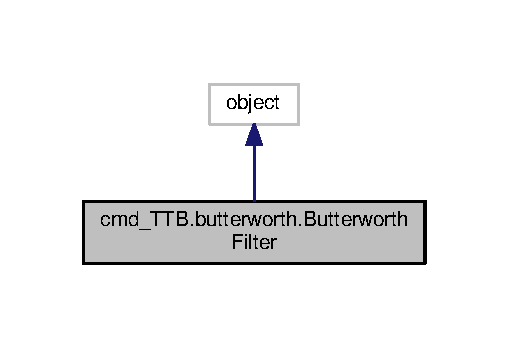
\includegraphics[width=244pt]{classcmd__TTB_1_1butterworth_1_1ButterworthFilter__inherit__graph}
\end{center}
\end{figure}


Collaboration diagram for cmd\+\_\+\+T\+T\+B.\+butterworth.\+Butterworth\+Filter\+:\nopagebreak
\begin{figure}[H]
\begin{center}
\leavevmode
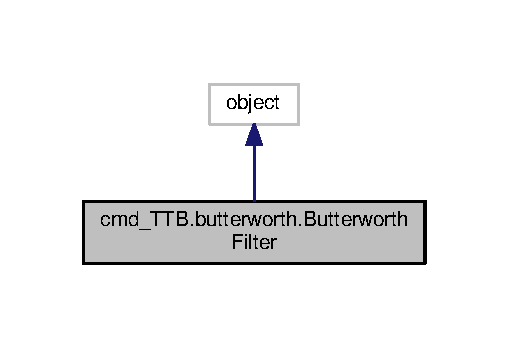
\includegraphics[width=244pt]{classcmd__TTB_1_1butterworth_1_1ButterworthFilter__coll__graph}
\end{center}
\end{figure}
\subsection*{Public Member Functions}
\begin{DoxyCompactItemize}
\item 
def \hyperlink{classcmd__TTB_1_1butterworth_1_1ButterworthFilter_a8f569482d8099798494dc38a16589f8f}{\+\_\+\+\_\+init\+\_\+\+\_\+} (self)
\item 
def \hyperlink{classcmd__TTB_1_1butterworth_1_1ButterworthFilter_a770af7ed4ce5ed48fc9db1d42ca0b588}{filter} (self, lastY, newY, lastX, newX, last\+Theta, new\+Theta, F\+R\+EQ, u\+Instantaneous=0)
\begin{DoxyCompactList}\small\item\em Return the linear and angular velocities estimated from the values of the pose of the robot, the frequency and the linear velocity estimated by TT (which is unreliable). \end{DoxyCompactList}\end{DoxyCompactItemize}
\subsection*{Public Attributes}
\begin{DoxyCompactItemize}
\item 
\hyperlink{classcmd__TTB_1_1butterworth_1_1ButterworthFilter_ad8a64b6be0a7b11ab2626affc4df0955}{w\+Filtered\+\_\+prec}
\item 
\hyperlink{classcmd__TTB_1_1butterworth_1_1ButterworthFilter_aa31176200eee925ee48f575d6d5acc9e}{w\+Filtered}
\item 
\hyperlink{classcmd__TTB_1_1butterworth_1_1ButterworthFilter_a112d92005652f64e47664227b5cf3c73}{w\+Raw\+\_\+prec}
\item 
\hyperlink{classcmd__TTB_1_1butterworth_1_1ButterworthFilter_a967096c3f7f90d51ee25cabe6153c67c}{w\+Brut}
\begin{DoxyCompactList}\small\item\em w\+Brut \+: angular speed before applying Butterworth \end{DoxyCompactList}\item 
\hyperlink{classcmd__TTB_1_1butterworth_1_1ButterworthFilter_a72fb79f01a2e947721335436d2cfdaa7}{atan2lifter}
\item 
\hyperlink{classcmd__TTB_1_1butterworth_1_1ButterworthFilter_ab699cd8db314b9845544edcf90efccc7}{u\+Filtered\+\_\+prec}
\item 
\hyperlink{classcmd__TTB_1_1butterworth_1_1ButterworthFilter_a1193cc0d35e56c0758e36ccdea45cfd4}{u\+Filtered}
\item 
\hyperlink{classcmd__TTB_1_1butterworth_1_1ButterworthFilter_abadf344eae18ac29ab1b8f2784fef116}{u\+Raw\+\_\+prec}
\item 
\hyperlink{classcmd__TTB_1_1butterworth_1_1ButterworthFilter_a0f4537c092a3823d6285cffd5e2b825f}{u\+Raw}
\begin{DoxyCompactList}\small\item\em u\+Raw \+: linear speed before applying Butterworth \end{DoxyCompactList}\item 
\hyperlink{classcmd__TTB_1_1butterworth_1_1ButterworthFilter_a45ae1004420f2101ad51feec56ae595d}{theta\+Init}
\end{DoxyCompactItemize}


\subsection{Constructor \& Destructor Documentation}
\index{cmd\+\_\+\+T\+T\+B\+::butterworth\+::\+Butterworth\+Filter@{cmd\+\_\+\+T\+T\+B\+::butterworth\+::\+Butterworth\+Filter}!\+\_\+\+\_\+init\+\_\+\+\_\+@{\+\_\+\+\_\+init\+\_\+\+\_\+}}
\index{\+\_\+\+\_\+init\+\_\+\+\_\+@{\+\_\+\+\_\+init\+\_\+\+\_\+}!cmd\+\_\+\+T\+T\+B\+::butterworth\+::\+Butterworth\+Filter@{cmd\+\_\+\+T\+T\+B\+::butterworth\+::\+Butterworth\+Filter}}
\subsubsection[{\texorpdfstring{\+\_\+\+\_\+init\+\_\+\+\_\+(self)}{__init__(self)}}]{\setlength{\rightskip}{0pt plus 5cm}def cmd\+\_\+\+T\+T\+B.\+butterworth.\+Butterworth\+Filter.\+\_\+\+\_\+init\+\_\+\+\_\+ (
\begin{DoxyParamCaption}
\item[{}]{self}
\end{DoxyParamCaption}
)}\hypertarget{classcmd__TTB_1_1butterworth_1_1ButterworthFilter_a8f569482d8099798494dc38a16589f8f}{}\label{classcmd__TTB_1_1butterworth_1_1ButterworthFilter_a8f569482d8099798494dc38a16589f8f}


\subsection{Member Function Documentation}
\index{cmd\+\_\+\+T\+T\+B\+::butterworth\+::\+Butterworth\+Filter@{cmd\+\_\+\+T\+T\+B\+::butterworth\+::\+Butterworth\+Filter}!filter@{filter}}
\index{filter@{filter}!cmd\+\_\+\+T\+T\+B\+::butterworth\+::\+Butterworth\+Filter@{cmd\+\_\+\+T\+T\+B\+::butterworth\+::\+Butterworth\+Filter}}
\subsubsection[{\texorpdfstring{filter(self, last\+Y, new\+Y, last\+X, new\+X, last\+Theta, new\+Theta, F\+R\+E\+Q, u\+Instantaneous=0)}{filter(self, lastY, newY, lastX, newX, lastTheta, newTheta, FREQ, uInstantaneous=0)}}]{\setlength{\rightskip}{0pt plus 5cm}def cmd\+\_\+\+T\+T\+B.\+butterworth.\+Butterworth\+Filter.\+filter (
\begin{DoxyParamCaption}
\item[{}]{self, }
\item[{}]{lastY, }
\item[{}]{newY, }
\item[{}]{lastX, }
\item[{}]{newX, }
\item[{}]{last\+Theta, }
\item[{}]{new\+Theta, }
\item[{}]{F\+R\+EQ, }
\item[{}]{u\+Instantaneous = {\ttfamily 0}}
\end{DoxyParamCaption}
)}\hypertarget{classcmd__TTB_1_1butterworth_1_1ButterworthFilter_a770af7ed4ce5ed48fc9db1d42ca0b588}{}\label{classcmd__TTB_1_1butterworth_1_1ButterworthFilter_a770af7ed4ce5ed48fc9db1d42ca0b588}


Return the linear and angular velocities estimated from the values of the pose of the robot, the frequency and the linear velocity estimated by TT (which is unreliable). 



\subsection{Member Data Documentation}
\index{cmd\+\_\+\+T\+T\+B\+::butterworth\+::\+Butterworth\+Filter@{cmd\+\_\+\+T\+T\+B\+::butterworth\+::\+Butterworth\+Filter}!atan2lifter@{atan2lifter}}
\index{atan2lifter@{atan2lifter}!cmd\+\_\+\+T\+T\+B\+::butterworth\+::\+Butterworth\+Filter@{cmd\+\_\+\+T\+T\+B\+::butterworth\+::\+Butterworth\+Filter}}
\subsubsection[{\texorpdfstring{atan2lifter}{atan2lifter}}]{\setlength{\rightskip}{0pt plus 5cm}cmd\+\_\+\+T\+T\+B.\+butterworth.\+Butterworth\+Filter.\+atan2lifter}\hypertarget{classcmd__TTB_1_1butterworth_1_1ButterworthFilter_a72fb79f01a2e947721335436d2cfdaa7}{}\label{classcmd__TTB_1_1butterworth_1_1ButterworthFilter_a72fb79f01a2e947721335436d2cfdaa7}
\index{cmd\+\_\+\+T\+T\+B\+::butterworth\+::\+Butterworth\+Filter@{cmd\+\_\+\+T\+T\+B\+::butterworth\+::\+Butterworth\+Filter}!theta\+Init@{theta\+Init}}
\index{theta\+Init@{theta\+Init}!cmd\+\_\+\+T\+T\+B\+::butterworth\+::\+Butterworth\+Filter@{cmd\+\_\+\+T\+T\+B\+::butterworth\+::\+Butterworth\+Filter}}
\subsubsection[{\texorpdfstring{theta\+Init}{thetaInit}}]{\setlength{\rightskip}{0pt plus 5cm}cmd\+\_\+\+T\+T\+B.\+butterworth.\+Butterworth\+Filter.\+theta\+Init}\hypertarget{classcmd__TTB_1_1butterworth_1_1ButterworthFilter_a45ae1004420f2101ad51feec56ae595d}{}\label{classcmd__TTB_1_1butterworth_1_1ButterworthFilter_a45ae1004420f2101ad51feec56ae595d}
\index{cmd\+\_\+\+T\+T\+B\+::butterworth\+::\+Butterworth\+Filter@{cmd\+\_\+\+T\+T\+B\+::butterworth\+::\+Butterworth\+Filter}!u\+Filtered@{u\+Filtered}}
\index{u\+Filtered@{u\+Filtered}!cmd\+\_\+\+T\+T\+B\+::butterworth\+::\+Butterworth\+Filter@{cmd\+\_\+\+T\+T\+B\+::butterworth\+::\+Butterworth\+Filter}}
\subsubsection[{\texorpdfstring{u\+Filtered}{uFiltered}}]{\setlength{\rightskip}{0pt plus 5cm}cmd\+\_\+\+T\+T\+B.\+butterworth.\+Butterworth\+Filter.\+u\+Filtered}\hypertarget{classcmd__TTB_1_1butterworth_1_1ButterworthFilter_a1193cc0d35e56c0758e36ccdea45cfd4}{}\label{classcmd__TTB_1_1butterworth_1_1ButterworthFilter_a1193cc0d35e56c0758e36ccdea45cfd4}
\index{cmd\+\_\+\+T\+T\+B\+::butterworth\+::\+Butterworth\+Filter@{cmd\+\_\+\+T\+T\+B\+::butterworth\+::\+Butterworth\+Filter}!u\+Filtered\+\_\+prec@{u\+Filtered\+\_\+prec}}
\index{u\+Filtered\+\_\+prec@{u\+Filtered\+\_\+prec}!cmd\+\_\+\+T\+T\+B\+::butterworth\+::\+Butterworth\+Filter@{cmd\+\_\+\+T\+T\+B\+::butterworth\+::\+Butterworth\+Filter}}
\subsubsection[{\texorpdfstring{u\+Filtered\+\_\+prec}{uFiltered_prec}}]{\setlength{\rightskip}{0pt plus 5cm}cmd\+\_\+\+T\+T\+B.\+butterworth.\+Butterworth\+Filter.\+u\+Filtered\+\_\+prec}\hypertarget{classcmd__TTB_1_1butterworth_1_1ButterworthFilter_ab699cd8db314b9845544edcf90efccc7}{}\label{classcmd__TTB_1_1butterworth_1_1ButterworthFilter_ab699cd8db314b9845544edcf90efccc7}
\index{cmd\+\_\+\+T\+T\+B\+::butterworth\+::\+Butterworth\+Filter@{cmd\+\_\+\+T\+T\+B\+::butterworth\+::\+Butterworth\+Filter}!u\+Raw@{u\+Raw}}
\index{u\+Raw@{u\+Raw}!cmd\+\_\+\+T\+T\+B\+::butterworth\+::\+Butterworth\+Filter@{cmd\+\_\+\+T\+T\+B\+::butterworth\+::\+Butterworth\+Filter}}
\subsubsection[{\texorpdfstring{u\+Raw}{uRaw}}]{\setlength{\rightskip}{0pt plus 5cm}cmd\+\_\+\+T\+T\+B.\+butterworth.\+Butterworth\+Filter.\+u\+Raw}\hypertarget{classcmd__TTB_1_1butterworth_1_1ButterworthFilter_a0f4537c092a3823d6285cffd5e2b825f}{}\label{classcmd__TTB_1_1butterworth_1_1ButterworthFilter_a0f4537c092a3823d6285cffd5e2b825f}


u\+Raw \+: linear speed before applying Butterworth 

\index{cmd\+\_\+\+T\+T\+B\+::butterworth\+::\+Butterworth\+Filter@{cmd\+\_\+\+T\+T\+B\+::butterworth\+::\+Butterworth\+Filter}!u\+Raw\+\_\+prec@{u\+Raw\+\_\+prec}}
\index{u\+Raw\+\_\+prec@{u\+Raw\+\_\+prec}!cmd\+\_\+\+T\+T\+B\+::butterworth\+::\+Butterworth\+Filter@{cmd\+\_\+\+T\+T\+B\+::butterworth\+::\+Butterworth\+Filter}}
\subsubsection[{\texorpdfstring{u\+Raw\+\_\+prec}{uRaw_prec}}]{\setlength{\rightskip}{0pt plus 5cm}cmd\+\_\+\+T\+T\+B.\+butterworth.\+Butterworth\+Filter.\+u\+Raw\+\_\+prec}\hypertarget{classcmd__TTB_1_1butterworth_1_1ButterworthFilter_abadf344eae18ac29ab1b8f2784fef116}{}\label{classcmd__TTB_1_1butterworth_1_1ButterworthFilter_abadf344eae18ac29ab1b8f2784fef116}
\index{cmd\+\_\+\+T\+T\+B\+::butterworth\+::\+Butterworth\+Filter@{cmd\+\_\+\+T\+T\+B\+::butterworth\+::\+Butterworth\+Filter}!w\+Brut@{w\+Brut}}
\index{w\+Brut@{w\+Brut}!cmd\+\_\+\+T\+T\+B\+::butterworth\+::\+Butterworth\+Filter@{cmd\+\_\+\+T\+T\+B\+::butterworth\+::\+Butterworth\+Filter}}
\subsubsection[{\texorpdfstring{w\+Brut}{wBrut}}]{\setlength{\rightskip}{0pt plus 5cm}cmd\+\_\+\+T\+T\+B.\+butterworth.\+Butterworth\+Filter.\+w\+Brut}\hypertarget{classcmd__TTB_1_1butterworth_1_1ButterworthFilter_a967096c3f7f90d51ee25cabe6153c67c}{}\label{classcmd__TTB_1_1butterworth_1_1ButterworthFilter_a967096c3f7f90d51ee25cabe6153c67c}


w\+Brut \+: angular speed before applying Butterworth 

\index{cmd\+\_\+\+T\+T\+B\+::butterworth\+::\+Butterworth\+Filter@{cmd\+\_\+\+T\+T\+B\+::butterworth\+::\+Butterworth\+Filter}!w\+Filtered@{w\+Filtered}}
\index{w\+Filtered@{w\+Filtered}!cmd\+\_\+\+T\+T\+B\+::butterworth\+::\+Butterworth\+Filter@{cmd\+\_\+\+T\+T\+B\+::butterworth\+::\+Butterworth\+Filter}}
\subsubsection[{\texorpdfstring{w\+Filtered}{wFiltered}}]{\setlength{\rightskip}{0pt plus 5cm}cmd\+\_\+\+T\+T\+B.\+butterworth.\+Butterworth\+Filter.\+w\+Filtered}\hypertarget{classcmd__TTB_1_1butterworth_1_1ButterworthFilter_aa31176200eee925ee48f575d6d5acc9e}{}\label{classcmd__TTB_1_1butterworth_1_1ButterworthFilter_aa31176200eee925ee48f575d6d5acc9e}
\index{cmd\+\_\+\+T\+T\+B\+::butterworth\+::\+Butterworth\+Filter@{cmd\+\_\+\+T\+T\+B\+::butterworth\+::\+Butterworth\+Filter}!w\+Filtered\+\_\+prec@{w\+Filtered\+\_\+prec}}
\index{w\+Filtered\+\_\+prec@{w\+Filtered\+\_\+prec}!cmd\+\_\+\+T\+T\+B\+::butterworth\+::\+Butterworth\+Filter@{cmd\+\_\+\+T\+T\+B\+::butterworth\+::\+Butterworth\+Filter}}
\subsubsection[{\texorpdfstring{w\+Filtered\+\_\+prec}{wFiltered_prec}}]{\setlength{\rightskip}{0pt plus 5cm}cmd\+\_\+\+T\+T\+B.\+butterworth.\+Butterworth\+Filter.\+w\+Filtered\+\_\+prec}\hypertarget{classcmd__TTB_1_1butterworth_1_1ButterworthFilter_ad8a64b6be0a7b11ab2626affc4df0955}{}\label{classcmd__TTB_1_1butterworth_1_1ButterworthFilter_ad8a64b6be0a7b11ab2626affc4df0955}
\index{cmd\+\_\+\+T\+T\+B\+::butterworth\+::\+Butterworth\+Filter@{cmd\+\_\+\+T\+T\+B\+::butterworth\+::\+Butterworth\+Filter}!w\+Raw\+\_\+prec@{w\+Raw\+\_\+prec}}
\index{w\+Raw\+\_\+prec@{w\+Raw\+\_\+prec}!cmd\+\_\+\+T\+T\+B\+::butterworth\+::\+Butterworth\+Filter@{cmd\+\_\+\+T\+T\+B\+::butterworth\+::\+Butterworth\+Filter}}
\subsubsection[{\texorpdfstring{w\+Raw\+\_\+prec}{wRaw_prec}}]{\setlength{\rightskip}{0pt plus 5cm}cmd\+\_\+\+T\+T\+B.\+butterworth.\+Butterworth\+Filter.\+w\+Raw\+\_\+prec}\hypertarget{classcmd__TTB_1_1butterworth_1_1ButterworthFilter_a112d92005652f64e47664227b5cf3c73}{}\label{classcmd__TTB_1_1butterworth_1_1ButterworthFilter_a112d92005652f64e47664227b5cf3c73}


The documentation for this class was generated from the following file\+:\begin{DoxyCompactItemize}
\item 
\hyperlink{butterworth_8py}{butterworth.\+py}\end{DoxyCompactItemize}

\hypertarget{classButterworthFilter}{}\section{Butterworth\+Filter Class Reference}
\label{classButterworthFilter}\index{Butterworth\+Filter@{Butterworth\+Filter}}


Estimator of the instantaneous velocities of the robot using a first order butterworth filter.  




\subsection{Detailed Description}
Estimator of the instantaneous velocities of the robot using a first order butterworth filter. 

The coefficients were chosen more or less randomly and should be optimised. 

The documentation for this class was generated from the following file\+:\begin{DoxyCompactItemize}
\item 
\hyperlink{butterworth_8py}{butterworth.\+py}\end{DoxyCompactItemize}

\hypertarget{classcmd__TTB_1_1dataGatherer_1_1DataGatherer}{}\section{cmd\+\_\+\+T\+T\+B.\+data\+Gatherer.\+Data\+Gatherer Class Reference}
\label{classcmd__TTB_1_1dataGatherer_1_1DataGatherer}\index{cmd\+\_\+\+T\+T\+B.\+data\+Gatherer.\+Data\+Gatherer@{cmd\+\_\+\+T\+T\+B.\+data\+Gatherer.\+Data\+Gatherer}}
\subsection*{Public Member Functions}
\begin{DoxyCompactItemize}
\item 
def \hyperlink{classcmd__TTB_1_1dataGatherer_1_1DataGatherer_acbea9abbb037555264b3c5d326560670}{\+\_\+\+\_\+init\+\_\+\+\_\+} (self, ttb\+Pose, vitesse\+Lineaire\+En\+Commande0, vitesse\+Angulaire\+En\+Commande0, F\+R\+E\+Q\+U\+E\+N\+CE)
\item 
def \hyperlink{classcmd__TTB_1_1dataGatherer_1_1DataGatherer_aa9c1979d72538a306c22fb573a0076b7}{new\+Command} (self, vitesse\+Lineaire\+En\+Commanden, vitesse\+Angulaire\+En\+Commanden)
\item 
def \hyperlink{classcmd__TTB_1_1dataGatherer_1_1DataGatherer_a22be32d8a6818d2bd0d0cfcc06d2d58f}{new\+Pos} (self, newX, newY, new\+Theta, vitesse\+Lineaire\+Instant=0)
\item 
def \hyperlink{classcmd__TTB_1_1dataGatherer_1_1DataGatherer_a2bf0a24ac3fc5a9a76bc1eefebf31334}{get\+InstantV} (self)
\item 
def \hyperlink{classcmd__TTB_1_1dataGatherer_1_1DataGatherer_a875c925135b3f187974f15a322f692aa}{get\+InstantW} (self)
\item 
def \hyperlink{classcmd__TTB_1_1dataGatherer_1_1DataGatherer_a1a6ea334eab99d499f23e05b68af46c1}{v} (self)
\item 
def \hyperlink{classcmd__TTB_1_1dataGatherer_1_1DataGatherer_ae41c1980d73278b1d973713988729b9d}{w} (self)
\item 
def \hyperlink{classcmd__TTB_1_1dataGatherer_1_1DataGatherer_adad43343ec9a615148fd26377eabc3b8}{to\+\_\+percent} (self, \hyperlink{classcmd__TTB_1_1dataGatherer_1_1DataGatherer_a3b8b2b639cad9c1192ef10efa68f2b51}{y}, position)
\item 
def \hyperlink{classcmd__TTB_1_1dataGatherer_1_1DataGatherer_a7fd8d77061ff08059ba8deea2d184d93}{save\+Data} (self)
\item 
def \hyperlink{classcmd__TTB_1_1dataGatherer_1_1DataGatherer_a55e8ac388f6a9e4ad794b8561559c52d}{Erreur} (self, consigne\+\_\+xy)
\item 
def \hyperlink{classcmd__TTB_1_1dataGatherer_1_1DataGatherer_a90a816bc1b190fda1e557c187eecb2a1}{errase} (self)
\item 
def \hyperlink{classcmd__TTB_1_1dataGatherer_1_1DataGatherer_a93a58d2eb75f586e0747278409fb8ef6}{plot} (self, v\+Reference, w\+Reference, consigne\+\_\+xy=None, consigne\+\_\+theta=0, porte=None)
\item 
def \hyperlink{classcmd__TTB_1_1dataGatherer_1_1DataGatherer_afe246ad25d224494702fcc6eaddf57fe}{plot\+Trajectory} (self, porte, position\+\_\+du\+\_\+repere)
\end{DoxyCompactItemize}
\subsection*{Public Attributes}
\begin{DoxyCompactItemize}
\item 
\hyperlink{classcmd__TTB_1_1dataGatherer_1_1DataGatherer_a088d7c0901296ea4bca154bab6c76aa9}{x}
\begin{DoxyCompactList}\small\item\em ---Initialisation de la position du robot mobile en x,y,theta \end{DoxyCompactList}\item 
\hyperlink{classcmd__TTB_1_1dataGatherer_1_1DataGatherer_a3b8b2b639cad9c1192ef10efa68f2b51}{y}
\item 
\hyperlink{classcmd__TTB_1_1dataGatherer_1_1DataGatherer_a5d41f95d517db30b08d462522c3d973a}{vitesse\+Lineaire}
\begin{DoxyCompactList}\small\item\em ---Initialisation des vitesses angulaires et lineaires, ces vitesses ne sont pas a modifier directement, elles sont recalculuee a chaque nouvelle pose \end{DoxyCompactList}\item 
\hyperlink{classcmd__TTB_1_1dataGatherer_1_1DataGatherer_afc9fa9a763fe0ff962f1fc9aa8e33e33}{vitesse\+Angulaire}
\item 
\hyperlink{classcmd__TTB_1_1dataGatherer_1_1DataGatherer_a096d1a4edcb1a9189ebfbea80cb646b5}{B\+W\+Filter}
\begin{DoxyCompactList}\small\item\em ---Initialisation du filtre de butterworth (estimateur des vitesses) \end{DoxyCompactList}\item 
\hyperlink{classcmd__TTB_1_1dataGatherer_1_1DataGatherer_a92c6e630cfff49229d514a0ea1a26ce1}{vitesse\+Lineaire\+En\+Commande}
\begin{DoxyCompactList}\small\item\em ---Initialisation des vitesses en commandes \end{DoxyCompactList}\item 
\hyperlink{classcmd__TTB_1_1dataGatherer_1_1DataGatherer_adf0b4f8826e0178d2a8fa681673f9284}{vitesse\+Angulaire\+En\+Commande}
\item 
\hyperlink{classcmd__TTB_1_1dataGatherer_1_1DataGatherer_a402999c8fcfdd46884f1afd92b3b2a9d}{t}
\begin{DoxyCompactList}\small\item\em ---Initialisation du tableau correspondant au t de chaque mesure \end{DoxyCompactList}\item 
\hyperlink{classcmd__TTB_1_1dataGatherer_1_1DataGatherer_ab3e9d78d3f2a56d97dc60dba0cd6e79d}{frequence}
\end{DoxyCompactItemize}
\subsection*{Static Public Attributes}
\begin{DoxyCompactItemize}
\item 
\hyperlink{classcmd__TTB_1_1dataGatherer_1_1DataGatherer_a695f502696fbf013ce1c9cda2c754917}{Vx} = np.\+gradient(self.\+y)
\item 
\hyperlink{classcmd__TTB_1_1dataGatherer_1_1DataGatherer_a8d9f9bc28acbf0f4a05a16222b2e450f}{theta} = np.\+array(self.\+theta);
\item 
\hyperlink{classcmd__TTB_1_1dataGatherer_1_1DataGatherer_a0f2d7b86e13cd53a7f357ac04fdf606c}{thetaV} = \hyperlink{namespacecmd__TTB_1_1utils_a59935c2b4ec8161367ca748f99c376cf}{utils.\+lifted\+Atan2}(\hyperlink{classcmd__TTB_1_1dataGatherer_1_1DataGatherer_a695f502696fbf013ce1c9cda2c754917}{Vx},Vy);
\item 
\hyperlink{classcmd__TTB_1_1dataGatherer_1_1DataGatherer_a70b267d03427145f555e919d3e2dc281}{v} = np.\+sqrt(\hyperlink{classcmd__TTB_1_1dataGatherer_1_1DataGatherer_a695f502696fbf013ce1c9cda2c754917}{Vx}$\ast$$\ast$2 + Vy$\ast$$\ast$2)$\ast$self.\+frequence
\end{DoxyCompactItemize}


\subsection{Constructor \& Destructor Documentation}
\index{cmd\+\_\+\+T\+T\+B\+::data\+Gatherer\+::\+Data\+Gatherer@{cmd\+\_\+\+T\+T\+B\+::data\+Gatherer\+::\+Data\+Gatherer}!\+\_\+\+\_\+init\+\_\+\+\_\+@{\+\_\+\+\_\+init\+\_\+\+\_\+}}
\index{\+\_\+\+\_\+init\+\_\+\+\_\+@{\+\_\+\+\_\+init\+\_\+\+\_\+}!cmd\+\_\+\+T\+T\+B\+::data\+Gatherer\+::\+Data\+Gatherer@{cmd\+\_\+\+T\+T\+B\+::data\+Gatherer\+::\+Data\+Gatherer}}
\subsubsection[{\texorpdfstring{\+\_\+\+\_\+init\+\_\+\+\_\+(self, ttb\+Pose, vitesse\+Lineaire\+En\+Commande0, vitesse\+Angulaire\+En\+Commande0, F\+R\+E\+Q\+U\+E\+N\+C\+E)}{__init__(self, ttbPose, vitesseLineaireEnCommande0, vitesseAngulaireEnCommande0, FREQUENCE)}}]{\setlength{\rightskip}{0pt plus 5cm}def cmd\+\_\+\+T\+T\+B.\+data\+Gatherer.\+Data\+Gatherer.\+\_\+\+\_\+init\+\_\+\+\_\+ (
\begin{DoxyParamCaption}
\item[{}]{self, }
\item[{}]{ttb\+Pose, }
\item[{}]{vitesse\+Lineaire\+En\+Commande0, }
\item[{}]{vitesse\+Angulaire\+En\+Commande0, }
\item[{}]{F\+R\+E\+Q\+U\+E\+N\+CE}
\end{DoxyParamCaption}
)}\hypertarget{classcmd__TTB_1_1dataGatherer_1_1DataGatherer_acbea9abbb037555264b3c5d326560670}{}\label{classcmd__TTB_1_1dataGatherer_1_1DataGatherer_acbea9abbb037555264b3c5d326560670}

\begin{DoxyParams}{Parameters}
{\em ttb\+Pose} & Pose2D Initial pose of the robot \\
\hline
{\em vitesse\+Lineaire\+En\+Commande0} & Double Initial linear speed \\
\hline
{\em vitesse\+Angulaire\+En\+Commande0} & Double Initial angular speed \\
\hline
{\em F\+R\+E\+Q\+U\+E\+N\+CE} & Double Frequence of the control law \\
\hline
\end{DoxyParams}


\subsection{Member Function Documentation}
\index{cmd\+\_\+\+T\+T\+B\+::data\+Gatherer\+::\+Data\+Gatherer@{cmd\+\_\+\+T\+T\+B\+::data\+Gatherer\+::\+Data\+Gatherer}!errase@{errase}}
\index{errase@{errase}!cmd\+\_\+\+T\+T\+B\+::data\+Gatherer\+::\+Data\+Gatherer@{cmd\+\_\+\+T\+T\+B\+::data\+Gatherer\+::\+Data\+Gatherer}}
\subsubsection[{\texorpdfstring{errase(self)}{errase(self)}}]{\setlength{\rightskip}{0pt plus 5cm}def cmd\+\_\+\+T\+T\+B.\+data\+Gatherer.\+Data\+Gatherer.\+errase (
\begin{DoxyParamCaption}
\item[{}]{self}
\end{DoxyParamCaption}
)}\hypertarget{classcmd__TTB_1_1dataGatherer_1_1DataGatherer_a90a816bc1b190fda1e557c187eecb2a1}{}\label{classcmd__TTB_1_1dataGatherer_1_1DataGatherer_a90a816bc1b190fda1e557c187eecb2a1}
\begin{DoxyVerb}Efface le contenu des listes du DataGatherer\end{DoxyVerb}
 \index{cmd\+\_\+\+T\+T\+B\+::data\+Gatherer\+::\+Data\+Gatherer@{cmd\+\_\+\+T\+T\+B\+::data\+Gatherer\+::\+Data\+Gatherer}!Erreur@{Erreur}}
\index{Erreur@{Erreur}!cmd\+\_\+\+T\+T\+B\+::data\+Gatherer\+::\+Data\+Gatherer@{cmd\+\_\+\+T\+T\+B\+::data\+Gatherer\+::\+Data\+Gatherer}}
\subsubsection[{\texorpdfstring{Erreur(self, consigne\+\_\+xy)}{Erreur(self, consigne_xy)}}]{\setlength{\rightskip}{0pt plus 5cm}def cmd\+\_\+\+T\+T\+B.\+data\+Gatherer.\+Data\+Gatherer.\+Erreur (
\begin{DoxyParamCaption}
\item[{}]{self, }
\item[{}]{consigne\+\_\+xy}
\end{DoxyParamCaption}
)}\hypertarget{classcmd__TTB_1_1dataGatherer_1_1DataGatherer_a55e8ac388f6a9e4ad794b8561559c52d}{}\label{classcmd__TTB_1_1dataGatherer_1_1DataGatherer_a55e8ac388f6a9e4ad794b8561559c52d}
\begin{DoxyVerb}Calcul l'erreur de position moyenne\end{DoxyVerb}
 \index{cmd\+\_\+\+T\+T\+B\+::data\+Gatherer\+::\+Data\+Gatherer@{cmd\+\_\+\+T\+T\+B\+::data\+Gatherer\+::\+Data\+Gatherer}!get\+InstantV@{get\+InstantV}}
\index{get\+InstantV@{get\+InstantV}!cmd\+\_\+\+T\+T\+B\+::data\+Gatherer\+::\+Data\+Gatherer@{cmd\+\_\+\+T\+T\+B\+::data\+Gatherer\+::\+Data\+Gatherer}}
\subsubsection[{\texorpdfstring{get\+Instant\+V(self)}{getInstantV(self)}}]{\setlength{\rightskip}{0pt plus 5cm}def cmd\+\_\+\+T\+T\+B.\+data\+Gatherer.\+Data\+Gatherer.\+get\+InstantV (
\begin{DoxyParamCaption}
\item[{}]{self}
\end{DoxyParamCaption}
)}\hypertarget{classcmd__TTB_1_1dataGatherer_1_1DataGatherer_a2bf0a24ac3fc5a9a76bc1eefebf31334}{}\label{classcmd__TTB_1_1dataGatherer_1_1DataGatherer_a2bf0a24ac3fc5a9a76bc1eefebf31334}
\begin{DoxyVerb}Retourne le dernier element de la liste des vitesses lineaires\end{DoxyVerb}
 \index{cmd\+\_\+\+T\+T\+B\+::data\+Gatherer\+::\+Data\+Gatherer@{cmd\+\_\+\+T\+T\+B\+::data\+Gatherer\+::\+Data\+Gatherer}!get\+InstantW@{get\+InstantW}}
\index{get\+InstantW@{get\+InstantW}!cmd\+\_\+\+T\+T\+B\+::data\+Gatherer\+::\+Data\+Gatherer@{cmd\+\_\+\+T\+T\+B\+::data\+Gatherer\+::\+Data\+Gatherer}}
\subsubsection[{\texorpdfstring{get\+Instant\+W(self)}{getInstantW(self)}}]{\setlength{\rightskip}{0pt plus 5cm}def cmd\+\_\+\+T\+T\+B.\+data\+Gatherer.\+Data\+Gatherer.\+get\+InstantW (
\begin{DoxyParamCaption}
\item[{}]{self}
\end{DoxyParamCaption}
)}\hypertarget{classcmd__TTB_1_1dataGatherer_1_1DataGatherer_a875c925135b3f187974f15a322f692aa}{}\label{classcmd__TTB_1_1dataGatherer_1_1DataGatherer_a875c925135b3f187974f15a322f692aa}
\begin{DoxyVerb}Retourne le dernier element de la liste des vitesses angulaires\end{DoxyVerb}
 \index{cmd\+\_\+\+T\+T\+B\+::data\+Gatherer\+::\+Data\+Gatherer@{cmd\+\_\+\+T\+T\+B\+::data\+Gatherer\+::\+Data\+Gatherer}!new\+Command@{new\+Command}}
\index{new\+Command@{new\+Command}!cmd\+\_\+\+T\+T\+B\+::data\+Gatherer\+::\+Data\+Gatherer@{cmd\+\_\+\+T\+T\+B\+::data\+Gatherer\+::\+Data\+Gatherer}}
\subsubsection[{\texorpdfstring{new\+Command(self, vitesse\+Lineaire\+En\+Commanden, vitesse\+Angulaire\+En\+Commanden)}{newCommand(self, vitesseLineaireEnCommanden, vitesseAngulaireEnCommanden)}}]{\setlength{\rightskip}{0pt plus 5cm}def cmd\+\_\+\+T\+T\+B.\+data\+Gatherer.\+Data\+Gatherer.\+new\+Command (
\begin{DoxyParamCaption}
\item[{}]{self, }
\item[{}]{vitesse\+Lineaire\+En\+Commanden, }
\item[{}]{vitesse\+Angulaire\+En\+Commanden}
\end{DoxyParamCaption}
)}\hypertarget{classcmd__TTB_1_1dataGatherer_1_1DataGatherer_aa9c1979d72538a306c22fb573a0076b7}{}\label{classcmd__TTB_1_1dataGatherer_1_1DataGatherer_aa9c1979d72538a306c22fb573a0076b7}
\begin{DoxyVerb}Stocke les dernieres commandes transmises au TTB, il est CONSEILLE de l'utiliser a chaque nouvelle mesure (i.e appel de la fonction newPos())\end{DoxyVerb}
 \index{cmd\+\_\+\+T\+T\+B\+::data\+Gatherer\+::\+Data\+Gatherer@{cmd\+\_\+\+T\+T\+B\+::data\+Gatherer\+::\+Data\+Gatherer}!new\+Pos@{new\+Pos}}
\index{new\+Pos@{new\+Pos}!cmd\+\_\+\+T\+T\+B\+::data\+Gatherer\+::\+Data\+Gatherer@{cmd\+\_\+\+T\+T\+B\+::data\+Gatherer\+::\+Data\+Gatherer}}
\subsubsection[{\texorpdfstring{new\+Pos(self, new\+X, new\+Y, new\+Theta, vitesse\+Lineaire\+Instant=0)}{newPos(self, newX, newY, newTheta, vitesseLineaireInstant=0)}}]{\setlength{\rightskip}{0pt plus 5cm}def cmd\+\_\+\+T\+T\+B.\+data\+Gatherer.\+Data\+Gatherer.\+new\+Pos (
\begin{DoxyParamCaption}
\item[{}]{self, }
\item[{}]{newX, }
\item[{}]{newY, }
\item[{}]{new\+Theta, }
\item[{}]{vitesse\+Lineaire\+Instant = {\ttfamily 0}}
\end{DoxyParamCaption}
)}\hypertarget{classcmd__TTB_1_1dataGatherer_1_1DataGatherer_a22be32d8a6818d2bd0d0cfcc06d2d58f}{}\label{classcmd__TTB_1_1dataGatherer_1_1DataGatherer_a22be32d8a6818d2bd0d0cfcc06d2d58f}
\begin{DoxyVerb}Stocke la derniere pose connue du TTB, il est CONSEILLE de l'utiliser le meme nombre de fois que newCommand()\end{DoxyVerb}
 \index{cmd\+\_\+\+T\+T\+B\+::data\+Gatherer\+::\+Data\+Gatherer@{cmd\+\_\+\+T\+T\+B\+::data\+Gatherer\+::\+Data\+Gatherer}!plot@{plot}}
\index{plot@{plot}!cmd\+\_\+\+T\+T\+B\+::data\+Gatherer\+::\+Data\+Gatherer@{cmd\+\_\+\+T\+T\+B\+::data\+Gatherer\+::\+Data\+Gatherer}}
\subsubsection[{\texorpdfstring{plot(self, v\+Reference, w\+Reference, consigne\+\_\+xy=\+None, consigne\+\_\+theta=0, porte=\+None)}{plot(self, vReference, wReference, consigne_xy=None, consigne_theta=0, porte=None)}}]{\setlength{\rightskip}{0pt plus 5cm}def cmd\+\_\+\+T\+T\+B.\+data\+Gatherer.\+Data\+Gatherer.\+plot (
\begin{DoxyParamCaption}
\item[{}]{self, }
\item[{}]{v\+Reference, }
\item[{}]{w\+Reference, }
\item[{}]{consigne\+\_\+xy = {\ttfamily None}, }
\item[{}]{consigne\+\_\+theta = {\ttfamily 0}, }
\item[{}]{porte = {\ttfamily None}}
\end{DoxyParamCaption}
)}\hypertarget{classcmd__TTB_1_1dataGatherer_1_1DataGatherer_a93a58d2eb75f586e0747278409fb8ef6}{}\label{classcmd__TTB_1_1dataGatherer_1_1DataGatherer_a93a58d2eb75f586e0747278409fb8ef6}
\index{cmd\+\_\+\+T\+T\+B\+::data\+Gatherer\+::\+Data\+Gatherer@{cmd\+\_\+\+T\+T\+B\+::data\+Gatherer\+::\+Data\+Gatherer}!plot\+Trajectory@{plot\+Trajectory}}
\index{plot\+Trajectory@{plot\+Trajectory}!cmd\+\_\+\+T\+T\+B\+::data\+Gatherer\+::\+Data\+Gatherer@{cmd\+\_\+\+T\+T\+B\+::data\+Gatherer\+::\+Data\+Gatherer}}
\subsubsection[{\texorpdfstring{plot\+Trajectory(self, porte, position\+\_\+du\+\_\+repere)}{plotTrajectory(self, porte, position_du_repere)}}]{\setlength{\rightskip}{0pt plus 5cm}def cmd\+\_\+\+T\+T\+B.\+data\+Gatherer.\+Data\+Gatherer.\+plot\+Trajectory (
\begin{DoxyParamCaption}
\item[{}]{self, }
\item[{}]{porte, }
\item[{}]{position\+\_\+du\+\_\+repere}
\end{DoxyParamCaption}
)}\hypertarget{classcmd__TTB_1_1dataGatherer_1_1DataGatherer_afe246ad25d224494702fcc6eaddf57fe}{}\label{classcmd__TTB_1_1dataGatherer_1_1DataGatherer_afe246ad25d224494702fcc6eaddf57fe}
\index{cmd\+\_\+\+T\+T\+B\+::data\+Gatherer\+::\+Data\+Gatherer@{cmd\+\_\+\+T\+T\+B\+::data\+Gatherer\+::\+Data\+Gatherer}!save\+Data@{save\+Data}}
\index{save\+Data@{save\+Data}!cmd\+\_\+\+T\+T\+B\+::data\+Gatherer\+::\+Data\+Gatherer@{cmd\+\_\+\+T\+T\+B\+::data\+Gatherer\+::\+Data\+Gatherer}}
\subsubsection[{\texorpdfstring{save\+Data(self)}{saveData(self)}}]{\setlength{\rightskip}{0pt plus 5cm}def cmd\+\_\+\+T\+T\+B.\+data\+Gatherer.\+Data\+Gatherer.\+save\+Data (
\begin{DoxyParamCaption}
\item[{}]{self}
\end{DoxyParamCaption}
)}\hypertarget{classcmd__TTB_1_1dataGatherer_1_1DataGatherer_a7fd8d77061ff08059ba8deea2d184d93}{}\label{classcmd__TTB_1_1dataGatherer_1_1DataGatherer_a7fd8d77061ff08059ba8deea2d184d93}
\begin{DoxyVerb}Enregistre les donnees dans un fichier output.txt, jamais vraiment utilisee, fonction a tester, a ameliorer ou a supprimer, Marc 07/08/2017 \end{DoxyVerb}
 \index{cmd\+\_\+\+T\+T\+B\+::data\+Gatherer\+::\+Data\+Gatherer@{cmd\+\_\+\+T\+T\+B\+::data\+Gatherer\+::\+Data\+Gatherer}!to\+\_\+percent@{to\+\_\+percent}}
\index{to\+\_\+percent@{to\+\_\+percent}!cmd\+\_\+\+T\+T\+B\+::data\+Gatherer\+::\+Data\+Gatherer@{cmd\+\_\+\+T\+T\+B\+::data\+Gatherer\+::\+Data\+Gatherer}}
\subsubsection[{\texorpdfstring{to\+\_\+percent(self, y, position)}{to_percent(self, y, position)}}]{\setlength{\rightskip}{0pt plus 5cm}def cmd\+\_\+\+T\+T\+B.\+data\+Gatherer.\+Data\+Gatherer.\+to\+\_\+percent (
\begin{DoxyParamCaption}
\item[{}]{self, }
\item[{}]{y, }
\item[{}]{position}
\end{DoxyParamCaption}
)}\hypertarget{classcmd__TTB_1_1dataGatherer_1_1DataGatherer_adad43343ec9a615148fd26377eabc3b8}{}\label{classcmd__TTB_1_1dataGatherer_1_1DataGatherer_adad43343ec9a615148fd26377eabc3b8}
\begin{DoxyVerb}fonction utilisee uniquement dans plot() pour le trace des histogrammes\end{DoxyVerb}
 \index{cmd\+\_\+\+T\+T\+B\+::data\+Gatherer\+::\+Data\+Gatherer@{cmd\+\_\+\+T\+T\+B\+::data\+Gatherer\+::\+Data\+Gatherer}!v@{v}}
\index{v@{v}!cmd\+\_\+\+T\+T\+B\+::data\+Gatherer\+::\+Data\+Gatherer@{cmd\+\_\+\+T\+T\+B\+::data\+Gatherer\+::\+Data\+Gatherer}}
\subsubsection[{\texorpdfstring{v(self)}{v(self)}}]{\setlength{\rightskip}{0pt plus 5cm}def cmd\+\_\+\+T\+T\+B.\+data\+Gatherer.\+Data\+Gatherer.\+v (
\begin{DoxyParamCaption}
\item[{}]{self}
\end{DoxyParamCaption}
)}\hypertarget{classcmd__TTB_1_1dataGatherer_1_1DataGatherer_a1a6ea334eab99d499f23e05b68af46c1}{}\label{classcmd__TTB_1_1dataGatherer_1_1DataGatherer_a1a6ea334eab99d499f23e05b68af46c1}
\begin{DoxyVerb}deprecated. Le signe de la vitesse lineaire est relativement imprevisible, fonction a eviter tant qu'elle ne sera pas corrigee, Marc 05/08/2017\end{DoxyVerb}
 \index{cmd\+\_\+\+T\+T\+B\+::data\+Gatherer\+::\+Data\+Gatherer@{cmd\+\_\+\+T\+T\+B\+::data\+Gatherer\+::\+Data\+Gatherer}!w@{w}}
\index{w@{w}!cmd\+\_\+\+T\+T\+B\+::data\+Gatherer\+::\+Data\+Gatherer@{cmd\+\_\+\+T\+T\+B\+::data\+Gatherer\+::\+Data\+Gatherer}}
\subsubsection[{\texorpdfstring{w(self)}{w(self)}}]{\setlength{\rightskip}{0pt plus 5cm}def cmd\+\_\+\+T\+T\+B.\+data\+Gatherer.\+Data\+Gatherer.\+w (
\begin{DoxyParamCaption}
\item[{}]{self}
\end{DoxyParamCaption}
)}\hypertarget{classcmd__TTB_1_1dataGatherer_1_1DataGatherer_ae41c1980d73278b1d973713988729b9d}{}\label{classcmd__TTB_1_1dataGatherer_1_1DataGatherer_ae41c1980d73278b1d973713988729b9d}
\begin{DoxyVerb}deprecated\end{DoxyVerb}
 

\subsection{Member Data Documentation}
\index{cmd\+\_\+\+T\+T\+B\+::data\+Gatherer\+::\+Data\+Gatherer@{cmd\+\_\+\+T\+T\+B\+::data\+Gatherer\+::\+Data\+Gatherer}!B\+W\+Filter@{B\+W\+Filter}}
\index{B\+W\+Filter@{B\+W\+Filter}!cmd\+\_\+\+T\+T\+B\+::data\+Gatherer\+::\+Data\+Gatherer@{cmd\+\_\+\+T\+T\+B\+::data\+Gatherer\+::\+Data\+Gatherer}}
\subsubsection[{\texorpdfstring{B\+W\+Filter}{BWFilter}}]{\setlength{\rightskip}{0pt plus 5cm}cmd\+\_\+\+T\+T\+B.\+data\+Gatherer.\+Data\+Gatherer.\+B\+W\+Filter}\hypertarget{classcmd__TTB_1_1dataGatherer_1_1DataGatherer_a096d1a4edcb1a9189ebfbea80cb646b5}{}\label{classcmd__TTB_1_1dataGatherer_1_1DataGatherer_a096d1a4edcb1a9189ebfbea80cb646b5}


---Initialisation du filtre de butterworth (estimateur des vitesses) 

\index{cmd\+\_\+\+T\+T\+B\+::data\+Gatherer\+::\+Data\+Gatherer@{cmd\+\_\+\+T\+T\+B\+::data\+Gatherer\+::\+Data\+Gatherer}!frequence@{frequence}}
\index{frequence@{frequence}!cmd\+\_\+\+T\+T\+B\+::data\+Gatherer\+::\+Data\+Gatherer@{cmd\+\_\+\+T\+T\+B\+::data\+Gatherer\+::\+Data\+Gatherer}}
\subsubsection[{\texorpdfstring{frequence}{frequence}}]{\setlength{\rightskip}{0pt plus 5cm}cmd\+\_\+\+T\+T\+B.\+data\+Gatherer.\+Data\+Gatherer.\+frequence}\hypertarget{classcmd__TTB_1_1dataGatherer_1_1DataGatherer_ab3e9d78d3f2a56d97dc60dba0cd6e79d}{}\label{classcmd__TTB_1_1dataGatherer_1_1DataGatherer_ab3e9d78d3f2a56d97dc60dba0cd6e79d}
\index{cmd\+\_\+\+T\+T\+B\+::data\+Gatherer\+::\+Data\+Gatherer@{cmd\+\_\+\+T\+T\+B\+::data\+Gatherer\+::\+Data\+Gatherer}!t@{t}}
\index{t@{t}!cmd\+\_\+\+T\+T\+B\+::data\+Gatherer\+::\+Data\+Gatherer@{cmd\+\_\+\+T\+T\+B\+::data\+Gatherer\+::\+Data\+Gatherer}}
\subsubsection[{\texorpdfstring{t}{t}}]{\setlength{\rightskip}{0pt plus 5cm}cmd\+\_\+\+T\+T\+B.\+data\+Gatherer.\+Data\+Gatherer.\+t}\hypertarget{classcmd__TTB_1_1dataGatherer_1_1DataGatherer_a402999c8fcfdd46884f1afd92b3b2a9d}{}\label{classcmd__TTB_1_1dataGatherer_1_1DataGatherer_a402999c8fcfdd46884f1afd92b3b2a9d}


---Initialisation du tableau correspondant au t de chaque mesure 

\index{cmd\+\_\+\+T\+T\+B\+::data\+Gatherer\+::\+Data\+Gatherer@{cmd\+\_\+\+T\+T\+B\+::data\+Gatherer\+::\+Data\+Gatherer}!theta@{theta}}
\index{theta@{theta}!cmd\+\_\+\+T\+T\+B\+::data\+Gatherer\+::\+Data\+Gatherer@{cmd\+\_\+\+T\+T\+B\+::data\+Gatherer\+::\+Data\+Gatherer}}
\subsubsection[{\texorpdfstring{theta}{theta}}]{\setlength{\rightskip}{0pt plus 5cm}cmd\+\_\+\+T\+T\+B.\+data\+Gatherer.\+Data\+Gatherer.\+theta = np.\+array(self.\+theta);\hspace{0.3cm}{\ttfamily [static]}}\hypertarget{classcmd__TTB_1_1dataGatherer_1_1DataGatherer_a8d9f9bc28acbf0f4a05a16222b2e450f}{}\label{classcmd__TTB_1_1dataGatherer_1_1DataGatherer_a8d9f9bc28acbf0f4a05a16222b2e450f}
\index{cmd\+\_\+\+T\+T\+B\+::data\+Gatherer\+::\+Data\+Gatherer@{cmd\+\_\+\+T\+T\+B\+::data\+Gatherer\+::\+Data\+Gatherer}!thetaV@{thetaV}}
\index{thetaV@{thetaV}!cmd\+\_\+\+T\+T\+B\+::data\+Gatherer\+::\+Data\+Gatherer@{cmd\+\_\+\+T\+T\+B\+::data\+Gatherer\+::\+Data\+Gatherer}}
\subsubsection[{\texorpdfstring{thetaV}{thetaV}}]{\setlength{\rightskip}{0pt plus 5cm}cmd\+\_\+\+T\+T\+B.\+data\+Gatherer.\+Data\+Gatherer.\+thetaV = {\bf utils.\+lifted\+Atan2}({\bf Vx},Vy);\hspace{0.3cm}{\ttfamily [static]}}\hypertarget{classcmd__TTB_1_1dataGatherer_1_1DataGatherer_a0f2d7b86e13cd53a7f357ac04fdf606c}{}\label{classcmd__TTB_1_1dataGatherer_1_1DataGatherer_a0f2d7b86e13cd53a7f357ac04fdf606c}
\index{cmd\+\_\+\+T\+T\+B\+::data\+Gatherer\+::\+Data\+Gatherer@{cmd\+\_\+\+T\+T\+B\+::data\+Gatherer\+::\+Data\+Gatherer}!v@{v}}
\index{v@{v}!cmd\+\_\+\+T\+T\+B\+::data\+Gatherer\+::\+Data\+Gatherer@{cmd\+\_\+\+T\+T\+B\+::data\+Gatherer\+::\+Data\+Gatherer}}
\subsubsection[{\texorpdfstring{v}{v}}]{\setlength{\rightskip}{0pt plus 5cm}cmd\+\_\+\+T\+T\+B.\+data\+Gatherer.\+Data\+Gatherer.\+v = np.\+sqrt({\bf Vx}$\ast$$\ast$2 + Vy$\ast$$\ast$2)$\ast$self.\+frequence\hspace{0.3cm}{\ttfamily [static]}}\hypertarget{classcmd__TTB_1_1dataGatherer_1_1DataGatherer_a70b267d03427145f555e919d3e2dc281}{}\label{classcmd__TTB_1_1dataGatherer_1_1DataGatherer_a70b267d03427145f555e919d3e2dc281}
\index{cmd\+\_\+\+T\+T\+B\+::data\+Gatherer\+::\+Data\+Gatherer@{cmd\+\_\+\+T\+T\+B\+::data\+Gatherer\+::\+Data\+Gatherer}!vitesse\+Angulaire@{vitesse\+Angulaire}}
\index{vitesse\+Angulaire@{vitesse\+Angulaire}!cmd\+\_\+\+T\+T\+B\+::data\+Gatherer\+::\+Data\+Gatherer@{cmd\+\_\+\+T\+T\+B\+::data\+Gatherer\+::\+Data\+Gatherer}}
\subsubsection[{\texorpdfstring{vitesse\+Angulaire}{vitesseAngulaire}}]{\setlength{\rightskip}{0pt plus 5cm}cmd\+\_\+\+T\+T\+B.\+data\+Gatherer.\+Data\+Gatherer.\+vitesse\+Angulaire}\hypertarget{classcmd__TTB_1_1dataGatherer_1_1DataGatherer_afc9fa9a763fe0ff962f1fc9aa8e33e33}{}\label{classcmd__TTB_1_1dataGatherer_1_1DataGatherer_afc9fa9a763fe0ff962f1fc9aa8e33e33}
\index{cmd\+\_\+\+T\+T\+B\+::data\+Gatherer\+::\+Data\+Gatherer@{cmd\+\_\+\+T\+T\+B\+::data\+Gatherer\+::\+Data\+Gatherer}!vitesse\+Angulaire\+En\+Commande@{vitesse\+Angulaire\+En\+Commande}}
\index{vitesse\+Angulaire\+En\+Commande@{vitesse\+Angulaire\+En\+Commande}!cmd\+\_\+\+T\+T\+B\+::data\+Gatherer\+::\+Data\+Gatherer@{cmd\+\_\+\+T\+T\+B\+::data\+Gatherer\+::\+Data\+Gatherer}}
\subsubsection[{\texorpdfstring{vitesse\+Angulaire\+En\+Commande}{vitesseAngulaireEnCommande}}]{\setlength{\rightskip}{0pt plus 5cm}cmd\+\_\+\+T\+T\+B.\+data\+Gatherer.\+Data\+Gatherer.\+vitesse\+Angulaire\+En\+Commande}\hypertarget{classcmd__TTB_1_1dataGatherer_1_1DataGatherer_adf0b4f8826e0178d2a8fa681673f9284}{}\label{classcmd__TTB_1_1dataGatherer_1_1DataGatherer_adf0b4f8826e0178d2a8fa681673f9284}
\index{cmd\+\_\+\+T\+T\+B\+::data\+Gatherer\+::\+Data\+Gatherer@{cmd\+\_\+\+T\+T\+B\+::data\+Gatherer\+::\+Data\+Gatherer}!vitesse\+Lineaire@{vitesse\+Lineaire}}
\index{vitesse\+Lineaire@{vitesse\+Lineaire}!cmd\+\_\+\+T\+T\+B\+::data\+Gatherer\+::\+Data\+Gatherer@{cmd\+\_\+\+T\+T\+B\+::data\+Gatherer\+::\+Data\+Gatherer}}
\subsubsection[{\texorpdfstring{vitesse\+Lineaire}{vitesseLineaire}}]{\setlength{\rightskip}{0pt plus 5cm}cmd\+\_\+\+T\+T\+B.\+data\+Gatherer.\+Data\+Gatherer.\+vitesse\+Lineaire}\hypertarget{classcmd__TTB_1_1dataGatherer_1_1DataGatherer_a5d41f95d517db30b08d462522c3d973a}{}\label{classcmd__TTB_1_1dataGatherer_1_1DataGatherer_a5d41f95d517db30b08d462522c3d973a}


---Initialisation des vitesses angulaires et lineaires, ces vitesses ne sont pas a modifier directement, elles sont recalculuee a chaque nouvelle pose 

\index{cmd\+\_\+\+T\+T\+B\+::data\+Gatherer\+::\+Data\+Gatherer@{cmd\+\_\+\+T\+T\+B\+::data\+Gatherer\+::\+Data\+Gatherer}!vitesse\+Lineaire\+En\+Commande@{vitesse\+Lineaire\+En\+Commande}}
\index{vitesse\+Lineaire\+En\+Commande@{vitesse\+Lineaire\+En\+Commande}!cmd\+\_\+\+T\+T\+B\+::data\+Gatherer\+::\+Data\+Gatherer@{cmd\+\_\+\+T\+T\+B\+::data\+Gatherer\+::\+Data\+Gatherer}}
\subsubsection[{\texorpdfstring{vitesse\+Lineaire\+En\+Commande}{vitesseLineaireEnCommande}}]{\setlength{\rightskip}{0pt plus 5cm}cmd\+\_\+\+T\+T\+B.\+data\+Gatherer.\+Data\+Gatherer.\+vitesse\+Lineaire\+En\+Commande}\hypertarget{classcmd__TTB_1_1dataGatherer_1_1DataGatherer_a92c6e630cfff49229d514a0ea1a26ce1}{}\label{classcmd__TTB_1_1dataGatherer_1_1DataGatherer_a92c6e630cfff49229d514a0ea1a26ce1}


---Initialisation des vitesses en commandes 

\index{cmd\+\_\+\+T\+T\+B\+::data\+Gatherer\+::\+Data\+Gatherer@{cmd\+\_\+\+T\+T\+B\+::data\+Gatherer\+::\+Data\+Gatherer}!Vx@{Vx}}
\index{Vx@{Vx}!cmd\+\_\+\+T\+T\+B\+::data\+Gatherer\+::\+Data\+Gatherer@{cmd\+\_\+\+T\+T\+B\+::data\+Gatherer\+::\+Data\+Gatherer}}
\subsubsection[{\texorpdfstring{Vx}{Vx}}]{\setlength{\rightskip}{0pt plus 5cm}cmd\+\_\+\+T\+T\+B.\+data\+Gatherer.\+Data\+Gatherer.\+Vx = np.\+gradient(self.\+y)\hspace{0.3cm}{\ttfamily [static]}}\hypertarget{classcmd__TTB_1_1dataGatherer_1_1DataGatherer_a695f502696fbf013ce1c9cda2c754917}{}\label{classcmd__TTB_1_1dataGatherer_1_1DataGatherer_a695f502696fbf013ce1c9cda2c754917}
\index{cmd\+\_\+\+T\+T\+B\+::data\+Gatherer\+::\+Data\+Gatherer@{cmd\+\_\+\+T\+T\+B\+::data\+Gatherer\+::\+Data\+Gatherer}!x@{x}}
\index{x@{x}!cmd\+\_\+\+T\+T\+B\+::data\+Gatherer\+::\+Data\+Gatherer@{cmd\+\_\+\+T\+T\+B\+::data\+Gatherer\+::\+Data\+Gatherer}}
\subsubsection[{\texorpdfstring{x}{x}}]{\setlength{\rightskip}{0pt plus 5cm}cmd\+\_\+\+T\+T\+B.\+data\+Gatherer.\+Data\+Gatherer.\+x}\hypertarget{classcmd__TTB_1_1dataGatherer_1_1DataGatherer_a088d7c0901296ea4bca154bab6c76aa9}{}\label{classcmd__TTB_1_1dataGatherer_1_1DataGatherer_a088d7c0901296ea4bca154bab6c76aa9}


---Initialisation de la position du robot mobile en x,y,theta 

\index{cmd\+\_\+\+T\+T\+B\+::data\+Gatherer\+::\+Data\+Gatherer@{cmd\+\_\+\+T\+T\+B\+::data\+Gatherer\+::\+Data\+Gatherer}!y@{y}}
\index{y@{y}!cmd\+\_\+\+T\+T\+B\+::data\+Gatherer\+::\+Data\+Gatherer@{cmd\+\_\+\+T\+T\+B\+::data\+Gatherer\+::\+Data\+Gatherer}}
\subsubsection[{\texorpdfstring{y}{y}}]{\setlength{\rightskip}{0pt plus 5cm}cmd\+\_\+\+T\+T\+B.\+data\+Gatherer.\+Data\+Gatherer.\+y}\hypertarget{classcmd__TTB_1_1dataGatherer_1_1DataGatherer_a3b8b2b639cad9c1192ef10efa68f2b51}{}\label{classcmd__TTB_1_1dataGatherer_1_1DataGatherer_a3b8b2b639cad9c1192ef10efa68f2b51}


The documentation for this class was generated from the following file\+:\begin{DoxyCompactItemize}
\item 
\hyperlink{dataGatherer_8py}{data\+Gatherer.\+py}\end{DoxyCompactItemize}

\hypertarget{classDataGatherer}{}\section{Data\+Gatherer Class Reference}
\label{classDataGatherer}\index{Data\+Gatherer@{Data\+Gatherer}}


Equivalent of a Log, this class regroup all datas and can plot them.  




\subsection{Detailed Description}
Equivalent of a Log, this class regroup all datas and can plot them. 

The documentation for this class was generated from the following file\+:\begin{DoxyCompactItemize}
\item 
\hyperlink{dataGatherer_8py}{data\+Gatherer.\+py}\end{DoxyCompactItemize}

\hypertarget{classcmd__TTB_1_1door_1_1Door}{}\section{cmd\+\_\+\+T\+T\+B.\+door.\+Door Class Reference}
\label{classcmd__TTB_1_1door_1_1Door}\index{cmd\+\_\+\+T\+T\+B.\+door.\+Door@{cmd\+\_\+\+T\+T\+B.\+door.\+Door}}
\subsection*{Public Member Functions}
\begin{DoxyCompactItemize}
\item 
def \hyperlink{classcmd__TTB_1_1door_1_1Door_aa56a9406385a9fb7d2b0a1d06a90d4da}{\+\_\+\+\_\+init\+\_\+\+\_\+} (self, \hyperlink{classcmd__TTB_1_1door_1_1Door_a43c4b1f6e9c6ae4187382dc263c58d02}{alpha}, \hyperlink{classcmd__TTB_1_1door_1_1Door_a067030e5b4755f2d2b4340588609901c}{wall\+Vector}, \hyperlink{classcmd__TTB_1_1door_1_1Door_a17ee5270094c8735cb4ae02968645fe2}{hinge\+Pose}, \hyperlink{classcmd__TTB_1_1door_1_1Door_ac11ebd7424dd4a074edcda4c0584e61d}{openning\+Dir}, \hyperlink{classcmd__TTB_1_1door_1_1Door_a212cc5247f91b1f69d35ae939c7ea34d}{geometry}=\mbox{[}\hyperlink{classcmd__TTB_1_1door_1_1Door_a82aed36f492d477c488cca0e31c91845}{l}, \hyperlink{classcmd__TTB_1_1door_1_1Door_a5366be26d44de1cad62c4aacb66718b1}{lp}, \hyperlink{classcmd__TTB_1_1door_1_1Door_aab6a2a8e488dad5304b7ee73e9ca65a9}{dis}, \hyperlink{classcmd__TTB_1_1door_1_1Door_a7802efbefd3ee0f39ad7da87db6bde66}{e}, \hyperlink{classcmd__TTB_1_1door_1_1Door_aeebd5ef44f3ec44c230c157e295b3414}{r\+T\+TB})
\item 
def \hyperlink{classcmd__TTB_1_1door_1_1Door_a813cada30a910799c7fc7722f25a015e}{change\+Alpha} (self, new\+Alpha)
\begin{DoxyCompactList}\small\item\em Set the new alpha value and makes it up-\/to-\/date. \end{DoxyCompactList}\item 
def \hyperlink{classcmd__TTB_1_1door_1_1Door_a78b3b6c52e6dc61fe481137d57d6b0c0}{compute\+Handles} (self)
\begin{DoxyCompactList}\small\item\em Return the positions of the handle. \end{DoxyCompactList}\item 
def \hyperlink{classcmd__TTB_1_1door_1_1Door_ac00b5e77ae2e82577bfd831248226fd2}{compute\+Door\+Vector} (self)
\begin{DoxyCompactList}\small\item\em Return the vector representing the door. \end{DoxyCompactList}\item 
def \hyperlink{classcmd__TTB_1_1door_1_1Door_a11ec42f1aae5d6e9216fb30f61b0f938}{set\+Handle\+Infos} (self, ttb\+Pose)
\begin{DoxyCompactList}\small\item\em Get the handle position and compute the vector between the two handles \+: handle\+Vector. \end{DoxyCompactList}\end{DoxyCompactItemize}
\subsection*{Public Attributes}
\begin{DoxyCompactItemize}
\item 
\hyperlink{classcmd__TTB_1_1door_1_1Door_a212cc5247f91b1f69d35ae939c7ea34d}{geometry}
\item 
\hyperlink{classcmd__TTB_1_1door_1_1Door_a82aed36f492d477c488cca0e31c91845}{l}
\item 
\hyperlink{classcmd__TTB_1_1door_1_1Door_a5366be26d44de1cad62c4aacb66718b1}{lp}
\item 
\hyperlink{classcmd__TTB_1_1door_1_1Door_aab6a2a8e488dad5304b7ee73e9ca65a9}{dis}
\item 
\hyperlink{classcmd__TTB_1_1door_1_1Door_a7802efbefd3ee0f39ad7da87db6bde66}{e}
\item 
\hyperlink{classcmd__TTB_1_1door_1_1Door_aeebd5ef44f3ec44c230c157e295b3414}{r\+T\+TB}
\item 
\hyperlink{classcmd__TTB_1_1door_1_1Door_a43c4b1f6e9c6ae4187382dc263c58d02}{alpha}
\item 
\hyperlink{classcmd__TTB_1_1door_1_1Door_a067030e5b4755f2d2b4340588609901c}{wall\+Vector}
\item 
\hyperlink{classcmd__TTB_1_1door_1_1Door_a17ee5270094c8735cb4ae02968645fe2}{hinge\+Pose}
\item 
\hyperlink{classcmd__TTB_1_1door_1_1Door_ac11ebd7424dd4a074edcda4c0584e61d}{openning\+Dir}
\item 
\hyperlink{classcmd__TTB_1_1door_1_1Door_aa7ead51645db4e5159f27f69d5aebc54}{door\+Vector}
\item 
\hyperlink{classcmd__TTB_1_1door_1_1Door_abf377a198959472e644f81d28abeee5f}{handles}
\item 
\hyperlink{classcmd__TTB_1_1door_1_1Door_a1bddc9ba7dbbb7d9e73ba75f3b3a7287}{handle\+Vector}
\item 
\hyperlink{classcmd__TTB_1_1door_1_1Door_a711d46f8f16b8142ee76f4e512e90953}{used\+Handle}
\end{DoxyCompactItemize}


\subsection{Constructor \& Destructor Documentation}
\index{cmd\+\_\+\+T\+T\+B\+::door\+::\+Door@{cmd\+\_\+\+T\+T\+B\+::door\+::\+Door}!\+\_\+\+\_\+init\+\_\+\+\_\+@{\+\_\+\+\_\+init\+\_\+\+\_\+}}
\index{\+\_\+\+\_\+init\+\_\+\+\_\+@{\+\_\+\+\_\+init\+\_\+\+\_\+}!cmd\+\_\+\+T\+T\+B\+::door\+::\+Door@{cmd\+\_\+\+T\+T\+B\+::door\+::\+Door}}
\subsubsection[{\texorpdfstring{\+\_\+\+\_\+init\+\_\+\+\_\+(self, alpha, wall\+Vector, hinge\+Pose, openning\+Dir, geometry=[l, lp, dis, e, r\+T\+T\+B)}{__init__(self, alpha, wallVector, hingePose, openningDir, geometry=[l, lp, dis, e, rTTB)}}]{\setlength{\rightskip}{0pt plus 5cm}def cmd\+\_\+\+T\+T\+B.\+door.\+Door.\+\_\+\+\_\+init\+\_\+\+\_\+ (
\begin{DoxyParamCaption}
\item[{}]{self, }
\item[{}]{alpha, }
\item[{}]{wall\+Vector, }
\item[{}]{hinge\+Pose, }
\item[{}]{openning\+Dir, }
\item[{}]{geometry = {\ttfamily \mbox{[}{\bf l}}, }
\item[{}]{lp, }
\item[{}]{dis, }
\item[{}]{e, }
\item[{}]{r\+T\+TB}
\end{DoxyParamCaption}
)}\hypertarget{classcmd__TTB_1_1door_1_1Door_aa56a9406385a9fb7d2b0a1d06a90d4da}{}\label{classcmd__TTB_1_1door_1_1Door_aa56a9406385a9fb7d2b0a1d06a90d4da}

\begin{DoxyParams}{Parameters}
{\em alpha} & Double \+: current opening angle of the door. This parameter isn\textquotesingle{}t updated in live \\
\hline
{\em wall\+Vector} & Vector defining the orientation of the door \\
\hline
{\em hinge\+Pose} & Array defining the hinge position in the global frame \\
\hline
{\em openning\+Dir} & Boolean \+: if true, the door opens in the trigonometric direction \\
\hline
{\em geometry} & Array containing the door geometry \\
\hline
\end{DoxyParams}


\subsection{Member Function Documentation}
\index{cmd\+\_\+\+T\+T\+B\+::door\+::\+Door@{cmd\+\_\+\+T\+T\+B\+::door\+::\+Door}!change\+Alpha@{change\+Alpha}}
\index{change\+Alpha@{change\+Alpha}!cmd\+\_\+\+T\+T\+B\+::door\+::\+Door@{cmd\+\_\+\+T\+T\+B\+::door\+::\+Door}}
\subsubsection[{\texorpdfstring{change\+Alpha(self, new\+Alpha)}{changeAlpha(self, newAlpha)}}]{\setlength{\rightskip}{0pt plus 5cm}def cmd\+\_\+\+T\+T\+B.\+door.\+Door.\+change\+Alpha (
\begin{DoxyParamCaption}
\item[{}]{self, }
\item[{}]{new\+Alpha}
\end{DoxyParamCaption}
)}\hypertarget{classcmd__TTB_1_1door_1_1Door_a813cada30a910799c7fc7722f25a015e}{}\label{classcmd__TTB_1_1door_1_1Door_a813cada30a910799c7fc7722f25a015e}


Set the new alpha value and makes it up-\/to-\/date. 


\begin{DoxyParams}{Parameters}
{\em new\+Alpha} & Double \+: new value of alpha. \\
\hline
\end{DoxyParams}
\index{cmd\+\_\+\+T\+T\+B\+::door\+::\+Door@{cmd\+\_\+\+T\+T\+B\+::door\+::\+Door}!compute\+Door\+Vector@{compute\+Door\+Vector}}
\index{compute\+Door\+Vector@{compute\+Door\+Vector}!cmd\+\_\+\+T\+T\+B\+::door\+::\+Door@{cmd\+\_\+\+T\+T\+B\+::door\+::\+Door}}
\subsubsection[{\texorpdfstring{compute\+Door\+Vector(self)}{computeDoorVector(self)}}]{\setlength{\rightskip}{0pt plus 5cm}def cmd\+\_\+\+T\+T\+B.\+door.\+Door.\+compute\+Door\+Vector (
\begin{DoxyParamCaption}
\item[{}]{self}
\end{DoxyParamCaption}
)}\hypertarget{classcmd__TTB_1_1door_1_1Door_ac00b5e77ae2e82577bfd831248226fd2}{}\label{classcmd__TTB_1_1door_1_1Door_ac00b5e77ae2e82577bfd831248226fd2}


Return the vector representing the door. 

\index{cmd\+\_\+\+T\+T\+B\+::door\+::\+Door@{cmd\+\_\+\+T\+T\+B\+::door\+::\+Door}!compute\+Handles@{compute\+Handles}}
\index{compute\+Handles@{compute\+Handles}!cmd\+\_\+\+T\+T\+B\+::door\+::\+Door@{cmd\+\_\+\+T\+T\+B\+::door\+::\+Door}}
\subsubsection[{\texorpdfstring{compute\+Handles(self)}{computeHandles(self)}}]{\setlength{\rightskip}{0pt plus 5cm}def cmd\+\_\+\+T\+T\+B.\+door.\+Door.\+compute\+Handles (
\begin{DoxyParamCaption}
\item[{}]{self}
\end{DoxyParamCaption}
)}\hypertarget{classcmd__TTB_1_1door_1_1Door_a78b3b6c52e6dc61fe481137d57d6b0c0}{}\label{classcmd__TTB_1_1door_1_1Door_a78b3b6c52e6dc61fe481137d57d6b0c0}


Return the positions of the handle. 

\index{cmd\+\_\+\+T\+T\+B\+::door\+::\+Door@{cmd\+\_\+\+T\+T\+B\+::door\+::\+Door}!set\+Handle\+Infos@{set\+Handle\+Infos}}
\index{set\+Handle\+Infos@{set\+Handle\+Infos}!cmd\+\_\+\+T\+T\+B\+::door\+::\+Door@{cmd\+\_\+\+T\+T\+B\+::door\+::\+Door}}
\subsubsection[{\texorpdfstring{set\+Handle\+Infos(self, ttb\+Pose)}{setHandleInfos(self, ttbPose)}}]{\setlength{\rightskip}{0pt plus 5cm}def cmd\+\_\+\+T\+T\+B.\+door.\+Door.\+set\+Handle\+Infos (
\begin{DoxyParamCaption}
\item[{}]{self, }
\item[{}]{ttb\+Pose}
\end{DoxyParamCaption}
)}\hypertarget{classcmd__TTB_1_1door_1_1Door_a11ec42f1aae5d6e9216fb30f61b0f938}{}\label{classcmd__TTB_1_1door_1_1Door_a11ec42f1aae5d6e9216fb30f61b0f938}


Get the handle position and compute the vector between the two handles \+: handle\+Vector. 


\begin{DoxyParams}{Parameters}
{\em ttb\+Pose} & Pose2D object containing the T\+TB\textquotesingle{}s pose\\
\hline
\end{DoxyParams}
Both handles positions are computed. The desired one is chosen as being the closest. The vector {\itshape handle\+Vector} is then computed as being the unit vector from the undesired handle to the desired one. \begin{DoxyWarning}{Warning}
\{Choosing the closest handle might not work in specific situations !\}. 
\end{DoxyWarning}


\subsection{Member Data Documentation}
\index{cmd\+\_\+\+T\+T\+B\+::door\+::\+Door@{cmd\+\_\+\+T\+T\+B\+::door\+::\+Door}!alpha@{alpha}}
\index{alpha@{alpha}!cmd\+\_\+\+T\+T\+B\+::door\+::\+Door@{cmd\+\_\+\+T\+T\+B\+::door\+::\+Door}}
\subsubsection[{\texorpdfstring{alpha}{alpha}}]{\setlength{\rightskip}{0pt plus 5cm}cmd\+\_\+\+T\+T\+B.\+door.\+Door.\+alpha}\hypertarget{classcmd__TTB_1_1door_1_1Door_a43c4b1f6e9c6ae4187382dc263c58d02}{}\label{classcmd__TTB_1_1door_1_1Door_a43c4b1f6e9c6ae4187382dc263c58d02}
\index{cmd\+\_\+\+T\+T\+B\+::door\+::\+Door@{cmd\+\_\+\+T\+T\+B\+::door\+::\+Door}!dis@{dis}}
\index{dis@{dis}!cmd\+\_\+\+T\+T\+B\+::door\+::\+Door@{cmd\+\_\+\+T\+T\+B\+::door\+::\+Door}}
\subsubsection[{\texorpdfstring{dis}{dis}}]{\setlength{\rightskip}{0pt plus 5cm}cmd\+\_\+\+T\+T\+B.\+door.\+Door.\+dis}\hypertarget{classcmd__TTB_1_1door_1_1Door_aab6a2a8e488dad5304b7ee73e9ca65a9}{}\label{classcmd__TTB_1_1door_1_1Door_aab6a2a8e488dad5304b7ee73e9ca65a9}
\index{cmd\+\_\+\+T\+T\+B\+::door\+::\+Door@{cmd\+\_\+\+T\+T\+B\+::door\+::\+Door}!door\+Vector@{door\+Vector}}
\index{door\+Vector@{door\+Vector}!cmd\+\_\+\+T\+T\+B\+::door\+::\+Door@{cmd\+\_\+\+T\+T\+B\+::door\+::\+Door}}
\subsubsection[{\texorpdfstring{door\+Vector}{doorVector}}]{\setlength{\rightskip}{0pt plus 5cm}cmd\+\_\+\+T\+T\+B.\+door.\+Door.\+door\+Vector}\hypertarget{classcmd__TTB_1_1door_1_1Door_aa7ead51645db4e5159f27f69d5aebc54}{}\label{classcmd__TTB_1_1door_1_1Door_aa7ead51645db4e5159f27f69d5aebc54}
\index{cmd\+\_\+\+T\+T\+B\+::door\+::\+Door@{cmd\+\_\+\+T\+T\+B\+::door\+::\+Door}!e@{e}}
\index{e@{e}!cmd\+\_\+\+T\+T\+B\+::door\+::\+Door@{cmd\+\_\+\+T\+T\+B\+::door\+::\+Door}}
\subsubsection[{\texorpdfstring{e}{e}}]{\setlength{\rightskip}{0pt plus 5cm}cmd\+\_\+\+T\+T\+B.\+door.\+Door.\+e}\hypertarget{classcmd__TTB_1_1door_1_1Door_a7802efbefd3ee0f39ad7da87db6bde66}{}\label{classcmd__TTB_1_1door_1_1Door_a7802efbefd3ee0f39ad7da87db6bde66}
\index{cmd\+\_\+\+T\+T\+B\+::door\+::\+Door@{cmd\+\_\+\+T\+T\+B\+::door\+::\+Door}!geometry@{geometry}}
\index{geometry@{geometry}!cmd\+\_\+\+T\+T\+B\+::door\+::\+Door@{cmd\+\_\+\+T\+T\+B\+::door\+::\+Door}}
\subsubsection[{\texorpdfstring{geometry}{geometry}}]{\setlength{\rightskip}{0pt plus 5cm}cmd\+\_\+\+T\+T\+B.\+door.\+Door.\+geometry}\hypertarget{classcmd__TTB_1_1door_1_1Door_a212cc5247f91b1f69d35ae939c7ea34d}{}\label{classcmd__TTB_1_1door_1_1Door_a212cc5247f91b1f69d35ae939c7ea34d}
\index{cmd\+\_\+\+T\+T\+B\+::door\+::\+Door@{cmd\+\_\+\+T\+T\+B\+::door\+::\+Door}!handles@{handles}}
\index{handles@{handles}!cmd\+\_\+\+T\+T\+B\+::door\+::\+Door@{cmd\+\_\+\+T\+T\+B\+::door\+::\+Door}}
\subsubsection[{\texorpdfstring{handles}{handles}}]{\setlength{\rightskip}{0pt plus 5cm}cmd\+\_\+\+T\+T\+B.\+door.\+Door.\+handles}\hypertarget{classcmd__TTB_1_1door_1_1Door_abf377a198959472e644f81d28abeee5f}{}\label{classcmd__TTB_1_1door_1_1Door_abf377a198959472e644f81d28abeee5f}
\index{cmd\+\_\+\+T\+T\+B\+::door\+::\+Door@{cmd\+\_\+\+T\+T\+B\+::door\+::\+Door}!handle\+Vector@{handle\+Vector}}
\index{handle\+Vector@{handle\+Vector}!cmd\+\_\+\+T\+T\+B\+::door\+::\+Door@{cmd\+\_\+\+T\+T\+B\+::door\+::\+Door}}
\subsubsection[{\texorpdfstring{handle\+Vector}{handleVector}}]{\setlength{\rightskip}{0pt plus 5cm}cmd\+\_\+\+T\+T\+B.\+door.\+Door.\+handle\+Vector}\hypertarget{classcmd__TTB_1_1door_1_1Door_a1bddc9ba7dbbb7d9e73ba75f3b3a7287}{}\label{classcmd__TTB_1_1door_1_1Door_a1bddc9ba7dbbb7d9e73ba75f3b3a7287}
\index{cmd\+\_\+\+T\+T\+B\+::door\+::\+Door@{cmd\+\_\+\+T\+T\+B\+::door\+::\+Door}!hinge\+Pose@{hinge\+Pose}}
\index{hinge\+Pose@{hinge\+Pose}!cmd\+\_\+\+T\+T\+B\+::door\+::\+Door@{cmd\+\_\+\+T\+T\+B\+::door\+::\+Door}}
\subsubsection[{\texorpdfstring{hinge\+Pose}{hingePose}}]{\setlength{\rightskip}{0pt plus 5cm}cmd\+\_\+\+T\+T\+B.\+door.\+Door.\+hinge\+Pose}\hypertarget{classcmd__TTB_1_1door_1_1Door_a17ee5270094c8735cb4ae02968645fe2}{}\label{classcmd__TTB_1_1door_1_1Door_a17ee5270094c8735cb4ae02968645fe2}
\index{cmd\+\_\+\+T\+T\+B\+::door\+::\+Door@{cmd\+\_\+\+T\+T\+B\+::door\+::\+Door}!l@{l}}
\index{l@{l}!cmd\+\_\+\+T\+T\+B\+::door\+::\+Door@{cmd\+\_\+\+T\+T\+B\+::door\+::\+Door}}
\subsubsection[{\texorpdfstring{l}{l}}]{\setlength{\rightskip}{0pt plus 5cm}cmd\+\_\+\+T\+T\+B.\+door.\+Door.\+l}\hypertarget{classcmd__TTB_1_1door_1_1Door_a82aed36f492d477c488cca0e31c91845}{}\label{classcmd__TTB_1_1door_1_1Door_a82aed36f492d477c488cca0e31c91845}
\index{cmd\+\_\+\+T\+T\+B\+::door\+::\+Door@{cmd\+\_\+\+T\+T\+B\+::door\+::\+Door}!lp@{lp}}
\index{lp@{lp}!cmd\+\_\+\+T\+T\+B\+::door\+::\+Door@{cmd\+\_\+\+T\+T\+B\+::door\+::\+Door}}
\subsubsection[{\texorpdfstring{lp}{lp}}]{\setlength{\rightskip}{0pt plus 5cm}cmd\+\_\+\+T\+T\+B.\+door.\+Door.\+lp}\hypertarget{classcmd__TTB_1_1door_1_1Door_a5366be26d44de1cad62c4aacb66718b1}{}\label{classcmd__TTB_1_1door_1_1Door_a5366be26d44de1cad62c4aacb66718b1}
\index{cmd\+\_\+\+T\+T\+B\+::door\+::\+Door@{cmd\+\_\+\+T\+T\+B\+::door\+::\+Door}!openning\+Dir@{openning\+Dir}}
\index{openning\+Dir@{openning\+Dir}!cmd\+\_\+\+T\+T\+B\+::door\+::\+Door@{cmd\+\_\+\+T\+T\+B\+::door\+::\+Door}}
\subsubsection[{\texorpdfstring{openning\+Dir}{openningDir}}]{\setlength{\rightskip}{0pt plus 5cm}cmd\+\_\+\+T\+T\+B.\+door.\+Door.\+openning\+Dir}\hypertarget{classcmd__TTB_1_1door_1_1Door_ac11ebd7424dd4a074edcda4c0584e61d}{}\label{classcmd__TTB_1_1door_1_1Door_ac11ebd7424dd4a074edcda4c0584e61d}
\index{cmd\+\_\+\+T\+T\+B\+::door\+::\+Door@{cmd\+\_\+\+T\+T\+B\+::door\+::\+Door}!r\+T\+TB@{r\+T\+TB}}
\index{r\+T\+TB@{r\+T\+TB}!cmd\+\_\+\+T\+T\+B\+::door\+::\+Door@{cmd\+\_\+\+T\+T\+B\+::door\+::\+Door}}
\subsubsection[{\texorpdfstring{r\+T\+TB}{rTTB}}]{\setlength{\rightskip}{0pt plus 5cm}cmd\+\_\+\+T\+T\+B.\+door.\+Door.\+r\+T\+TB}\hypertarget{classcmd__TTB_1_1door_1_1Door_aeebd5ef44f3ec44c230c157e295b3414}{}\label{classcmd__TTB_1_1door_1_1Door_aeebd5ef44f3ec44c230c157e295b3414}
\index{cmd\+\_\+\+T\+T\+B\+::door\+::\+Door@{cmd\+\_\+\+T\+T\+B\+::door\+::\+Door}!used\+Handle@{used\+Handle}}
\index{used\+Handle@{used\+Handle}!cmd\+\_\+\+T\+T\+B\+::door\+::\+Door@{cmd\+\_\+\+T\+T\+B\+::door\+::\+Door}}
\subsubsection[{\texorpdfstring{used\+Handle}{usedHandle}}]{\setlength{\rightskip}{0pt plus 5cm}cmd\+\_\+\+T\+T\+B.\+door.\+Door.\+used\+Handle}\hypertarget{classcmd__TTB_1_1door_1_1Door_a711d46f8f16b8142ee76f4e512e90953}{}\label{classcmd__TTB_1_1door_1_1Door_a711d46f8f16b8142ee76f4e512e90953}
\index{cmd\+\_\+\+T\+T\+B\+::door\+::\+Door@{cmd\+\_\+\+T\+T\+B\+::door\+::\+Door}!wall\+Vector@{wall\+Vector}}
\index{wall\+Vector@{wall\+Vector}!cmd\+\_\+\+T\+T\+B\+::door\+::\+Door@{cmd\+\_\+\+T\+T\+B\+::door\+::\+Door}}
\subsubsection[{\texorpdfstring{wall\+Vector}{wallVector}}]{\setlength{\rightskip}{0pt plus 5cm}cmd\+\_\+\+T\+T\+B.\+door.\+Door.\+wall\+Vector}\hypertarget{classcmd__TTB_1_1door_1_1Door_a067030e5b4755f2d2b4340588609901c}{}\label{classcmd__TTB_1_1door_1_1Door_a067030e5b4755f2d2b4340588609901c}


The documentation for this class was generated from the following file\+:\begin{DoxyCompactItemize}
\item 
\hyperlink{door_8py}{door.\+py}\end{DoxyCompactItemize}

\hypertarget{classDoor}{}\section{Door Class Reference}
\label{classDoor}\index{Door@{Door}}


This class contains all the elements necessary to define the door in the global frame.  




\subsection{Detailed Description}
This class contains all the elements necessary to define the door in the global frame. 

 

The documentation for this class was generated from the following file\+:\begin{DoxyCompactItemize}
\item 
\hyperlink{door_8py}{door.\+py}\end{DoxyCompactItemize}

\hypertarget{classPointCreator}{}\section{Point\+Creator Class Reference}
\label{classPointCreator}\index{Point\+Creator@{Point\+Creator}}


Creates the points necessary for computing the robot\textquotesingle{}s path.  




\subsection{Detailed Description}
Creates the points necessary for computing the robot\textquotesingle{}s path. 

Each step has its own function to compute points.


\begin{DoxyParams}{Parameters}
{\em door} & \hyperlink{classDoor}{Door} containing the parameters of the door \\
\hline
{\em ttb\+Pose} & Pose2D of the T\+TB at the beginning point \\
\hline
{\em stage} & String defining the current stage (go\+To\+Handle, move\+Door, etc.) \\
\hline
{\em step} & String defining the current step (face\+Handle, touch\+Handle, etc.) \\
\hline
{\em geometry} & Array containing the door geometry \\
\hline
\end{DoxyParams}


The documentation for this class was generated from the following file\+:\begin{DoxyCompactItemize}
\item 
\hyperlink{pointCreator_8py}{point\+Creator.\+py}\end{DoxyCompactItemize}

\hypertarget{classcmd__TTB_1_1pointCreator_1_1PointCreator}{}\section{cmd\+\_\+\+T\+T\+B.\+point\+Creator.\+Point\+Creator Class Reference}
\label{classcmd__TTB_1_1pointCreator_1_1PointCreator}\index{cmd\+\_\+\+T\+T\+B.\+point\+Creator.\+Point\+Creator@{cmd\+\_\+\+T\+T\+B.\+point\+Creator.\+Point\+Creator}}
\subsection*{Public Member Functions}
\begin{DoxyCompactItemize}
\item 
def \hyperlink{classcmd__TTB_1_1pointCreator_1_1PointCreator_a22aa433126ed8a208d6547016fe1e564}{\+\_\+\+\_\+init\+\_\+\+\_\+} (self, \hyperlink{classcmd__TTB_1_1pointCreator_1_1PointCreator_a7ed058c18c601c1c75dc7a0e965dc822}{c\+Door}, \hyperlink{classcmd__TTB_1_1pointCreator_1_1PointCreator_a21e4510de601ea33015ecd3b45cfafeb}{ttb\+Pose}, \hyperlink{classcmd__TTB_1_1pointCreator_1_1PointCreator_a33513665b686ce537a06fed0d6cb2eee}{stage}, \hyperlink{classcmd__TTB_1_1pointCreator_1_1PointCreator_a73d089e287c772c0f448da4b18b6d1ab}{step})
\item 
def \hyperlink{classcmd__TTB_1_1pointCreator_1_1PointCreator_a2efa5ee9b26fb53aac3f0b41f3d2ecda}{move\+Door\+Points} (self)
\begin{DoxyCompactList}\small\item\em Creates the points for the move\+Door stage. \end{DoxyCompactList}\item 
def \hyperlink{classcmd__TTB_1_1pointCreator_1_1PointCreator_a359567b295e7b7bb4b36fcb6bc962717}{go\+To\+Handle\+Points} (self)
\begin{DoxyCompactList}\small\item\em Creates the points for the face\+Handle and touch\+Handle steps. \end{DoxyCompactList}\item 
def \hyperlink{classcmd__TTB_1_1pointCreator_1_1PointCreator_af01910dd15edf3e018131ecbbfc5203f}{by\+Pass\+Door\+Points} (self)
\begin{DoxyCompactList}\small\item\em Creates the points for the \char`\"{}by\+Pass\+Door\char`\"{} step. \end{DoxyCompactList}\item 
def \hyperlink{classcmd__TTB_1_1pointCreator_1_1PointCreator_a0764b36d7a1d971835c3c8a110d78b91}{plot\+Map} (self, \hyperlink{classcmd__TTB_1_1pointCreator_1_1PointCreator_a59ce28204b76e1ab92e232ac4105933d}{points})
\begin{DoxyCompactList}\small\item\em Plot the map containing the robot, the door and the created points. \end{DoxyCompactList}\end{DoxyCompactItemize}
\subsection*{Public Attributes}
\begin{DoxyCompactItemize}
\item 
\hyperlink{classcmd__TTB_1_1pointCreator_1_1PointCreator_a7ed058c18c601c1c75dc7a0e965dc822}{c\+Door}
\item 
\hyperlink{classcmd__TTB_1_1pointCreator_1_1PointCreator_a21e4510de601ea33015ecd3b45cfafeb}{ttb\+Pose}
\item 
\hyperlink{classcmd__TTB_1_1pointCreator_1_1PointCreator_a33513665b686ce537a06fed0d6cb2eee}{stage}
\item 
\hyperlink{classcmd__TTB_1_1pointCreator_1_1PointCreator_a73d089e287c772c0f448da4b18b6d1ab}{step}
\item 
\hyperlink{classcmd__TTB_1_1pointCreator_1_1PointCreator_afc9a1fb971a47b8a825513922776e123}{initial\+Angle}
\item 
\hyperlink{classcmd__TTB_1_1pointCreator_1_1PointCreator_a59ce28204b76e1ab92e232ac4105933d}{points}
\end{DoxyCompactItemize}


\subsection{Constructor \& Destructor Documentation}
\index{cmd\+\_\+\+T\+T\+B\+::point\+Creator\+::\+Point\+Creator@{cmd\+\_\+\+T\+T\+B\+::point\+Creator\+::\+Point\+Creator}!\+\_\+\+\_\+init\+\_\+\+\_\+@{\+\_\+\+\_\+init\+\_\+\+\_\+}}
\index{\+\_\+\+\_\+init\+\_\+\+\_\+@{\+\_\+\+\_\+init\+\_\+\+\_\+}!cmd\+\_\+\+T\+T\+B\+::point\+Creator\+::\+Point\+Creator@{cmd\+\_\+\+T\+T\+B\+::point\+Creator\+::\+Point\+Creator}}
\subsubsection[{\texorpdfstring{\+\_\+\+\_\+init\+\_\+\+\_\+(self, c\+Door, ttb\+Pose, stage, step)}{__init__(self, cDoor, ttbPose, stage, step)}}]{\setlength{\rightskip}{0pt plus 5cm}def cmd\+\_\+\+T\+T\+B.\+point\+Creator.\+Point\+Creator.\+\_\+\+\_\+init\+\_\+\+\_\+ (
\begin{DoxyParamCaption}
\item[{}]{self, }
\item[{}]{c\+Door, }
\item[{}]{ttb\+Pose, }
\item[{}]{stage, }
\item[{}]{step}
\end{DoxyParamCaption}
)}\hypertarget{classcmd__TTB_1_1pointCreator_1_1PointCreator_a22aa433126ed8a208d6547016fe1e564}{}\label{classcmd__TTB_1_1pointCreator_1_1PointCreator_a22aa433126ed8a208d6547016fe1e564}


\subsection{Member Function Documentation}
\index{cmd\+\_\+\+T\+T\+B\+::point\+Creator\+::\+Point\+Creator@{cmd\+\_\+\+T\+T\+B\+::point\+Creator\+::\+Point\+Creator}!by\+Pass\+Door\+Points@{by\+Pass\+Door\+Points}}
\index{by\+Pass\+Door\+Points@{by\+Pass\+Door\+Points}!cmd\+\_\+\+T\+T\+B\+::point\+Creator\+::\+Point\+Creator@{cmd\+\_\+\+T\+T\+B\+::point\+Creator\+::\+Point\+Creator}}
\subsubsection[{\texorpdfstring{by\+Pass\+Door\+Points(self)}{byPassDoorPoints(self)}}]{\setlength{\rightskip}{0pt plus 5cm}def cmd\+\_\+\+T\+T\+B.\+point\+Creator.\+Point\+Creator.\+by\+Pass\+Door\+Points (
\begin{DoxyParamCaption}
\item[{}]{self}
\end{DoxyParamCaption}
)}\hypertarget{classcmd__TTB_1_1pointCreator_1_1PointCreator_af01910dd15edf3e018131ecbbfc5203f}{}\label{classcmd__TTB_1_1pointCreator_1_1PointCreator_af01910dd15edf3e018131ecbbfc5203f}


Creates the points for the \char`\"{}by\+Pass\+Door\char`\"{} step. 

\index{cmd\+\_\+\+T\+T\+B\+::point\+Creator\+::\+Point\+Creator@{cmd\+\_\+\+T\+T\+B\+::point\+Creator\+::\+Point\+Creator}!go\+To\+Handle\+Points@{go\+To\+Handle\+Points}}
\index{go\+To\+Handle\+Points@{go\+To\+Handle\+Points}!cmd\+\_\+\+T\+T\+B\+::point\+Creator\+::\+Point\+Creator@{cmd\+\_\+\+T\+T\+B\+::point\+Creator\+::\+Point\+Creator}}
\subsubsection[{\texorpdfstring{go\+To\+Handle\+Points(self)}{goToHandlePoints(self)}}]{\setlength{\rightskip}{0pt plus 5cm}def cmd\+\_\+\+T\+T\+B.\+point\+Creator.\+Point\+Creator.\+go\+To\+Handle\+Points (
\begin{DoxyParamCaption}
\item[{}]{self}
\end{DoxyParamCaption}
)}\hypertarget{classcmd__TTB_1_1pointCreator_1_1PointCreator_a359567b295e7b7bb4b36fcb6bc962717}{}\label{classcmd__TTB_1_1pointCreator_1_1PointCreator_a359567b295e7b7bb4b36fcb6bc962717}


Creates the points for the face\+Handle and touch\+Handle steps. 

\index{cmd\+\_\+\+T\+T\+B\+::point\+Creator\+::\+Point\+Creator@{cmd\+\_\+\+T\+T\+B\+::point\+Creator\+::\+Point\+Creator}!move\+Door\+Points@{move\+Door\+Points}}
\index{move\+Door\+Points@{move\+Door\+Points}!cmd\+\_\+\+T\+T\+B\+::point\+Creator\+::\+Point\+Creator@{cmd\+\_\+\+T\+T\+B\+::point\+Creator\+::\+Point\+Creator}}
\subsubsection[{\texorpdfstring{move\+Door\+Points(self)}{moveDoorPoints(self)}}]{\setlength{\rightskip}{0pt plus 5cm}def cmd\+\_\+\+T\+T\+B.\+point\+Creator.\+Point\+Creator.\+move\+Door\+Points (
\begin{DoxyParamCaption}
\item[{}]{self}
\end{DoxyParamCaption}
)}\hypertarget{classcmd__TTB_1_1pointCreator_1_1PointCreator_a2efa5ee9b26fb53aac3f0b41f3d2ecda}{}\label{classcmd__TTB_1_1pointCreator_1_1PointCreator_a2efa5ee9b26fb53aac3f0b41f3d2ecda}


Creates the points for the move\+Door stage. 

\index{cmd\+\_\+\+T\+T\+B\+::point\+Creator\+::\+Point\+Creator@{cmd\+\_\+\+T\+T\+B\+::point\+Creator\+::\+Point\+Creator}!plot\+Map@{plot\+Map}}
\index{plot\+Map@{plot\+Map}!cmd\+\_\+\+T\+T\+B\+::point\+Creator\+::\+Point\+Creator@{cmd\+\_\+\+T\+T\+B\+::point\+Creator\+::\+Point\+Creator}}
\subsubsection[{\texorpdfstring{plot\+Map(self, points)}{plotMap(self, points)}}]{\setlength{\rightskip}{0pt plus 5cm}def cmd\+\_\+\+T\+T\+B.\+point\+Creator.\+Point\+Creator.\+plot\+Map (
\begin{DoxyParamCaption}
\item[{}]{self, }
\item[{}]{points}
\end{DoxyParamCaption}
)}\hypertarget{classcmd__TTB_1_1pointCreator_1_1PointCreator_a0764b36d7a1d971835c3c8a110d78b91}{}\label{classcmd__TTB_1_1pointCreator_1_1PointCreator_a0764b36d7a1d971835c3c8a110d78b91}


Plot the map containing the robot, the door and the created points. 



\subsection{Member Data Documentation}
\index{cmd\+\_\+\+T\+T\+B\+::point\+Creator\+::\+Point\+Creator@{cmd\+\_\+\+T\+T\+B\+::point\+Creator\+::\+Point\+Creator}!c\+Door@{c\+Door}}
\index{c\+Door@{c\+Door}!cmd\+\_\+\+T\+T\+B\+::point\+Creator\+::\+Point\+Creator@{cmd\+\_\+\+T\+T\+B\+::point\+Creator\+::\+Point\+Creator}}
\subsubsection[{\texorpdfstring{c\+Door}{cDoor}}]{\setlength{\rightskip}{0pt plus 5cm}cmd\+\_\+\+T\+T\+B.\+point\+Creator.\+Point\+Creator.\+c\+Door}\hypertarget{classcmd__TTB_1_1pointCreator_1_1PointCreator_a7ed058c18c601c1c75dc7a0e965dc822}{}\label{classcmd__TTB_1_1pointCreator_1_1PointCreator_a7ed058c18c601c1c75dc7a0e965dc822}
\index{cmd\+\_\+\+T\+T\+B\+::point\+Creator\+::\+Point\+Creator@{cmd\+\_\+\+T\+T\+B\+::point\+Creator\+::\+Point\+Creator}!initial\+Angle@{initial\+Angle}}
\index{initial\+Angle@{initial\+Angle}!cmd\+\_\+\+T\+T\+B\+::point\+Creator\+::\+Point\+Creator@{cmd\+\_\+\+T\+T\+B\+::point\+Creator\+::\+Point\+Creator}}
\subsubsection[{\texorpdfstring{initial\+Angle}{initialAngle}}]{\setlength{\rightskip}{0pt plus 5cm}cmd\+\_\+\+T\+T\+B.\+point\+Creator.\+Point\+Creator.\+initial\+Angle}\hypertarget{classcmd__TTB_1_1pointCreator_1_1PointCreator_afc9a1fb971a47b8a825513922776e123}{}\label{classcmd__TTB_1_1pointCreator_1_1PointCreator_afc9a1fb971a47b8a825513922776e123}
\index{cmd\+\_\+\+T\+T\+B\+::point\+Creator\+::\+Point\+Creator@{cmd\+\_\+\+T\+T\+B\+::point\+Creator\+::\+Point\+Creator}!points@{points}}
\index{points@{points}!cmd\+\_\+\+T\+T\+B\+::point\+Creator\+::\+Point\+Creator@{cmd\+\_\+\+T\+T\+B\+::point\+Creator\+::\+Point\+Creator}}
\subsubsection[{\texorpdfstring{points}{points}}]{\setlength{\rightskip}{0pt plus 5cm}cmd\+\_\+\+T\+T\+B.\+point\+Creator.\+Point\+Creator.\+points}\hypertarget{classcmd__TTB_1_1pointCreator_1_1PointCreator_a59ce28204b76e1ab92e232ac4105933d}{}\label{classcmd__TTB_1_1pointCreator_1_1PointCreator_a59ce28204b76e1ab92e232ac4105933d}
\index{cmd\+\_\+\+T\+T\+B\+::point\+Creator\+::\+Point\+Creator@{cmd\+\_\+\+T\+T\+B\+::point\+Creator\+::\+Point\+Creator}!stage@{stage}}
\index{stage@{stage}!cmd\+\_\+\+T\+T\+B\+::point\+Creator\+::\+Point\+Creator@{cmd\+\_\+\+T\+T\+B\+::point\+Creator\+::\+Point\+Creator}}
\subsubsection[{\texorpdfstring{stage}{stage}}]{\setlength{\rightskip}{0pt plus 5cm}cmd\+\_\+\+T\+T\+B.\+point\+Creator.\+Point\+Creator.\+stage}\hypertarget{classcmd__TTB_1_1pointCreator_1_1PointCreator_a33513665b686ce537a06fed0d6cb2eee}{}\label{classcmd__TTB_1_1pointCreator_1_1PointCreator_a33513665b686ce537a06fed0d6cb2eee}
\index{cmd\+\_\+\+T\+T\+B\+::point\+Creator\+::\+Point\+Creator@{cmd\+\_\+\+T\+T\+B\+::point\+Creator\+::\+Point\+Creator}!step@{step}}
\index{step@{step}!cmd\+\_\+\+T\+T\+B\+::point\+Creator\+::\+Point\+Creator@{cmd\+\_\+\+T\+T\+B\+::point\+Creator\+::\+Point\+Creator}}
\subsubsection[{\texorpdfstring{step}{step}}]{\setlength{\rightskip}{0pt plus 5cm}cmd\+\_\+\+T\+T\+B.\+point\+Creator.\+Point\+Creator.\+step}\hypertarget{classcmd__TTB_1_1pointCreator_1_1PointCreator_a73d089e287c772c0f448da4b18b6d1ab}{}\label{classcmd__TTB_1_1pointCreator_1_1PointCreator_a73d089e287c772c0f448da4b18b6d1ab}
\index{cmd\+\_\+\+T\+T\+B\+::point\+Creator\+::\+Point\+Creator@{cmd\+\_\+\+T\+T\+B\+::point\+Creator\+::\+Point\+Creator}!ttb\+Pose@{ttb\+Pose}}
\index{ttb\+Pose@{ttb\+Pose}!cmd\+\_\+\+T\+T\+B\+::point\+Creator\+::\+Point\+Creator@{cmd\+\_\+\+T\+T\+B\+::point\+Creator\+::\+Point\+Creator}}
\subsubsection[{\texorpdfstring{ttb\+Pose}{ttbPose}}]{\setlength{\rightskip}{0pt plus 5cm}cmd\+\_\+\+T\+T\+B.\+point\+Creator.\+Point\+Creator.\+ttb\+Pose}\hypertarget{classcmd__TTB_1_1pointCreator_1_1PointCreator_a21e4510de601ea33015ecd3b45cfafeb}{}\label{classcmd__TTB_1_1pointCreator_1_1PointCreator_a21e4510de601ea33015ecd3b45cfafeb}


The documentation for this class was generated from the following file\+:\begin{DoxyCompactItemize}
\item 
\hyperlink{pointCreator_8py}{point\+Creator.\+py}\end{DoxyCompactItemize}

\hypertarget{classSmoother}{}\section{Smoother Class Reference}
\label{classSmoother}\index{Smoother@{Smoother}}


The only purpose of this class is to suppress the discontinuities resulting from the computing of arctan, and \char`\"{}lifting\char`\"{} theta.  




\subsection{Detailed Description}
The only purpose of this class is to suppress the discontinuities resulting from the computing of arctan, and \char`\"{}lifting\char`\"{} theta. 

\begin{DoxyWarning}{Warning}
\{Might be useless and there is no need to use a class !\} 
\end{DoxyWarning}


The documentation for this class was generated from the following file\+:\begin{DoxyCompactItemize}
\item 
\hyperlink{utils_8py}{utils.\+py}\end{DoxyCompactItemize}

\hypertarget{classcmd__TTB_1_1utils_1_1Smoother}{}\section{cmd\+\_\+\+T\+T\+B.\+utils.\+Smoother Class Reference}
\label{classcmd__TTB_1_1utils_1_1Smoother}\index{cmd\+\_\+\+T\+T\+B.\+utils.\+Smoother@{cmd\+\_\+\+T\+T\+B.\+utils.\+Smoother}}
\subsection*{Public Member Functions}
\begin{DoxyCompactItemize}
\item 
def \hyperlink{classcmd__TTB_1_1utils_1_1Smoother_a890222ee3f4262589ee0ccffd4e73459}{\+\_\+\+\_\+init\+\_\+\+\_\+} (self, value\+List=list())
\item 
def \hyperlink{classcmd__TTB_1_1utils_1_1Smoother_abdf6af1fe2b9009de09a80f854a6a1cb}{new\+Val} (self, Value)
\end{DoxyCompactItemize}
\subsection*{Public Attributes}
\begin{DoxyCompactItemize}
\item 
\hyperlink{classcmd__TTB_1_1utils_1_1Smoother_a1a6a53aebf4a90db690d8ee2e5b57a78}{Classic\+Shortlist}
\item 
\hyperlink{classcmd__TTB_1_1utils_1_1Smoother_aabd258f9a6defa05dfc72c09b15bc5b3}{Classic\+Exceptionlist}
\item 
\hyperlink{classcmd__TTB_1_1utils_1_1Smoother_a17a6be1aa09cfc3a8fe9fd690f83612f}{Second\+Exceptionlist}
\end{DoxyCompactItemize}


\subsection{Constructor \& Destructor Documentation}
\index{cmd\+\_\+\+T\+T\+B\+::utils\+::\+Smoother@{cmd\+\_\+\+T\+T\+B\+::utils\+::\+Smoother}!\+\_\+\+\_\+init\+\_\+\+\_\+@{\+\_\+\+\_\+init\+\_\+\+\_\+}}
\index{\+\_\+\+\_\+init\+\_\+\+\_\+@{\+\_\+\+\_\+init\+\_\+\+\_\+}!cmd\+\_\+\+T\+T\+B\+::utils\+::\+Smoother@{cmd\+\_\+\+T\+T\+B\+::utils\+::\+Smoother}}
\subsubsection[{\texorpdfstring{\+\_\+\+\_\+init\+\_\+\+\_\+(self, value\+List=list())}{__init__(self, valueList=list())}}]{\setlength{\rightskip}{0pt plus 5cm}def cmd\+\_\+\+T\+T\+B.\+utils.\+Smoother.\+\_\+\+\_\+init\+\_\+\+\_\+ (
\begin{DoxyParamCaption}
\item[{}]{self, }
\item[{}]{value\+List = {\ttfamily list()}}
\end{DoxyParamCaption}
)}\hypertarget{classcmd__TTB_1_1utils_1_1Smoother_a890222ee3f4262589ee0ccffd4e73459}{}\label{classcmd__TTB_1_1utils_1_1Smoother_a890222ee3f4262589ee0ccffd4e73459}


\subsection{Member Function Documentation}
\index{cmd\+\_\+\+T\+T\+B\+::utils\+::\+Smoother@{cmd\+\_\+\+T\+T\+B\+::utils\+::\+Smoother}!new\+Val@{new\+Val}}
\index{new\+Val@{new\+Val}!cmd\+\_\+\+T\+T\+B\+::utils\+::\+Smoother@{cmd\+\_\+\+T\+T\+B\+::utils\+::\+Smoother}}
\subsubsection[{\texorpdfstring{new\+Val(self, Value)}{newVal(self, Value)}}]{\setlength{\rightskip}{0pt plus 5cm}def cmd\+\_\+\+T\+T\+B.\+utils.\+Smoother.\+new\+Val (
\begin{DoxyParamCaption}
\item[{}]{self, }
\item[{}]{Value}
\end{DoxyParamCaption}
)}\hypertarget{classcmd__TTB_1_1utils_1_1Smoother_abdf6af1fe2b9009de09a80f854a6a1cb}{}\label{classcmd__TTB_1_1utils_1_1Smoother_abdf6af1fe2b9009de09a80f854a6a1cb}


\subsection{Member Data Documentation}
\index{cmd\+\_\+\+T\+T\+B\+::utils\+::\+Smoother@{cmd\+\_\+\+T\+T\+B\+::utils\+::\+Smoother}!Classic\+Exceptionlist@{Classic\+Exceptionlist}}
\index{Classic\+Exceptionlist@{Classic\+Exceptionlist}!cmd\+\_\+\+T\+T\+B\+::utils\+::\+Smoother@{cmd\+\_\+\+T\+T\+B\+::utils\+::\+Smoother}}
\subsubsection[{\texorpdfstring{Classic\+Exceptionlist}{ClassicExceptionlist}}]{\setlength{\rightskip}{0pt plus 5cm}cmd\+\_\+\+T\+T\+B.\+utils.\+Smoother.\+Classic\+Exceptionlist}\hypertarget{classcmd__TTB_1_1utils_1_1Smoother_aabd258f9a6defa05dfc72c09b15bc5b3}{}\label{classcmd__TTB_1_1utils_1_1Smoother_aabd258f9a6defa05dfc72c09b15bc5b3}
\index{cmd\+\_\+\+T\+T\+B\+::utils\+::\+Smoother@{cmd\+\_\+\+T\+T\+B\+::utils\+::\+Smoother}!Classic\+Shortlist@{Classic\+Shortlist}}
\index{Classic\+Shortlist@{Classic\+Shortlist}!cmd\+\_\+\+T\+T\+B\+::utils\+::\+Smoother@{cmd\+\_\+\+T\+T\+B\+::utils\+::\+Smoother}}
\subsubsection[{\texorpdfstring{Classic\+Shortlist}{ClassicShortlist}}]{\setlength{\rightskip}{0pt plus 5cm}cmd\+\_\+\+T\+T\+B.\+utils.\+Smoother.\+Classic\+Shortlist}\hypertarget{classcmd__TTB_1_1utils_1_1Smoother_a1a6a53aebf4a90db690d8ee2e5b57a78}{}\label{classcmd__TTB_1_1utils_1_1Smoother_a1a6a53aebf4a90db690d8ee2e5b57a78}
\index{cmd\+\_\+\+T\+T\+B\+::utils\+::\+Smoother@{cmd\+\_\+\+T\+T\+B\+::utils\+::\+Smoother}!Second\+Exceptionlist@{Second\+Exceptionlist}}
\index{Second\+Exceptionlist@{Second\+Exceptionlist}!cmd\+\_\+\+T\+T\+B\+::utils\+::\+Smoother@{cmd\+\_\+\+T\+T\+B\+::utils\+::\+Smoother}}
\subsubsection[{\texorpdfstring{Second\+Exceptionlist}{SecondExceptionlist}}]{\setlength{\rightskip}{0pt plus 5cm}cmd\+\_\+\+T\+T\+B.\+utils.\+Smoother.\+Second\+Exceptionlist}\hypertarget{classcmd__TTB_1_1utils_1_1Smoother_a17a6be1aa09cfc3a8fe9fd690f83612f}{}\label{classcmd__TTB_1_1utils_1_1Smoother_a17a6be1aa09cfc3a8fe9fd690f83612f}


The documentation for this class was generated from the following file\+:\begin{DoxyCompactItemize}
\item 
\hyperlink{utils_8py}{utils.\+py}\end{DoxyCompactItemize}

\hypertarget{classcmd__TTB_1_1controllers_1_1TrajectoryStabilisator}{}\section{cmd\+\_\+\+T\+T\+B.\+controllers.\+Trajectory\+Stabilisator Class Reference}
\label{classcmd__TTB_1_1controllers_1_1TrajectoryStabilisator}\index{cmd\+\_\+\+T\+T\+B.\+controllers.\+Trajectory\+Stabilisator@{cmd\+\_\+\+T\+T\+B.\+controllers.\+Trajectory\+Stabilisator}}


Inheritance diagram for cmd\+\_\+\+T\+T\+B.\+controllers.\+Trajectory\+Stabilisator\+:\nopagebreak
\begin{figure}[H]
\begin{center}
\leavevmode
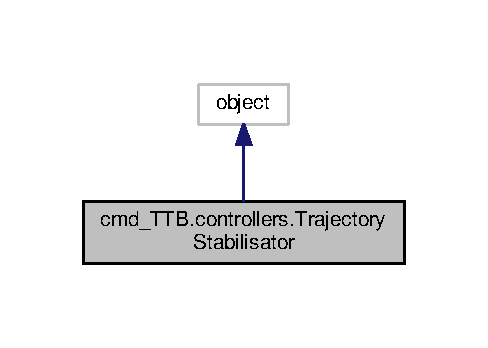
\includegraphics[width=234pt]{classcmd__TTB_1_1controllers_1_1TrajectoryStabilisator__inherit__graph}
\end{center}
\end{figure}


Collaboration diagram for cmd\+\_\+\+T\+T\+B.\+controllers.\+Trajectory\+Stabilisator\+:\nopagebreak
\begin{figure}[H]
\begin{center}
\leavevmode
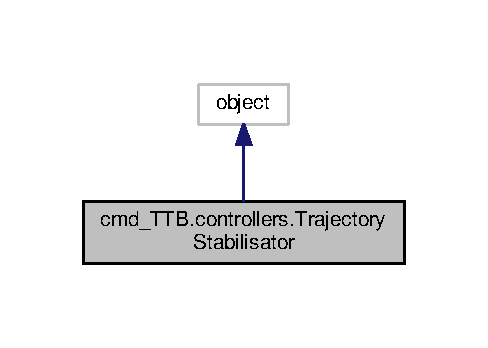
\includegraphics[width=234pt]{classcmd__TTB_1_1controllers_1_1TrajectoryStabilisator__coll__graph}
\end{center}
\end{figure}
\subsection*{Public Member Functions}
\begin{DoxyCompactItemize}
\item 
def \hyperlink{classcmd__TTB_1_1controllers_1_1TrajectoryStabilisator_ad42379fbbd0ec30bdc425e81fd47611f}{\+\_\+\+\_\+init\+\_\+\+\_\+} (self, \hyperlink{classcmd__TTB_1_1controllers_1_1TrajectoryStabilisator_a6eb1c01d0f7628c9c55aba2e1c1a5f87}{consigne\+\_\+xy}, \hyperlink{classcmd__TTB_1_1controllers_1_1TrajectoryStabilisator_a8a5025ec66995976f3c7bd6d976cb426}{consigne\+\_\+theta}, \hyperlink{classcmd__TTB_1_1controllers_1_1TrajectoryStabilisator_a7aacf24b292c214b7507ed7ff775d9d8}{consigne\+\_\+v}, \hyperlink{classcmd__TTB_1_1controllers_1_1TrajectoryStabilisator_a66ceabf25b6fc0f738457520d8a6b72d}{consigne\+\_\+w}, \hyperlink{classcmd__TTB_1_1controllers_1_1TrajectoryStabilisator_aedda44c52c85b3984f4c58b4d6157575}{F\+R\+EQ}, \hyperlink{classcmd__TTB_1_1controllers_1_1TrajectoryStabilisator_a82d3c2d639861e91f72560750417920e}{k1}=0, \hyperlink{classcmd__TTB_1_1controllers_1_1TrajectoryStabilisator_af96b6610b96e8a7d036848bf168c2c01}{k2}=0, \hyperlink{classcmd__TTB_1_1controllers_1_1TrajectoryStabilisator_abe267c474aea918130fd31fdfe818938}{k3}=0)
\item 
def \hyperlink{classcmd__TTB_1_1controllers_1_1TrajectoryStabilisator_a7a3a50c500ed52611cfc72a5d1e0804d}{get\+VW} (self, x, y, theta, k)
\begin{DoxyCompactList}\small\item\em Returns the velocities v and w based on the robot\textquotesingle{}s pose (x,y,theta) \end{DoxyCompactList}\item 
def \hyperlink{classcmd__TTB_1_1controllers_1_1TrajectoryStabilisator_aa4adb81d4e63a8d861722a62806638c7}{avoid\+Singularity} (self, theta, k)
\begin{DoxyCompactList}\small\item\em Having theta=0 (which is not allowed by \hyperlink{classcmd__TTB_1_1controllers_1_1TrajectoryStabilisator_a554b57b36fcb2f9f1d0b87058ed9992e}{get\+Cmd}). \end{DoxyCompactList}\item 
def \hyperlink{classcmd__TTB_1_1controllers_1_1TrajectoryStabilisator_a9dba372897104d13678ed72114abd7e8}{get\+State} (self, x, y, theta, k)
\begin{DoxyCompactList}\small\item\em Get the system\textquotesingle{}s state (tracking errors) which is the measured positions minus the reference. \end{DoxyCompactList}\item 
def \hyperlink{classcmd__TTB_1_1controllers_1_1TrajectoryStabilisator_a554b57b36fcb2f9f1d0b87058ed9992e}{get\+Cmd} (self, x1, x2, x3, k)
\begin{DoxyCompactList}\small\item\em Computes the first control law (u1, u2) from the system\textquotesingle{}s state (tracking errors) \end{DoxyCompactList}\item 
def \hyperlink{classcmd__TTB_1_1controllers_1_1TrajectoryStabilisator_a273938caf148ebbb4f720dec76dc3aa2}{get\+Output} (self, x3, u1, u2, k)
\begin{DoxyCompactList}\small\item\em Computes the second control law (v, w) from the system\textquotesingle{}s state (tracking errors) and the orientation error x3. \end{DoxyCompactList}\end{DoxyCompactItemize}
\subsection*{Public Attributes}
\begin{DoxyCompactItemize}
\item 
\hyperlink{classcmd__TTB_1_1controllers_1_1TrajectoryStabilisator_a6eb1c01d0f7628c9c55aba2e1c1a5f87}{consigne\+\_\+xy}
\item 
\hyperlink{classcmd__TTB_1_1controllers_1_1TrajectoryStabilisator_a8a5025ec66995976f3c7bd6d976cb426}{consigne\+\_\+theta}
\item 
\hyperlink{classcmd__TTB_1_1controllers_1_1TrajectoryStabilisator_a7aacf24b292c214b7507ed7ff775d9d8}{consigne\+\_\+v}
\item 
\hyperlink{classcmd__TTB_1_1controllers_1_1TrajectoryStabilisator_a66ceabf25b6fc0f738457520d8a6b72d}{consigne\+\_\+w}
\item 
\hyperlink{classcmd__TTB_1_1controllers_1_1TrajectoryStabilisator_aedda44c52c85b3984f4c58b4d6157575}{F\+R\+EQ}
\item 
\hyperlink{classcmd__TTB_1_1controllers_1_1TrajectoryStabilisator_a82d3c2d639861e91f72560750417920e}{k1}
\item 
\hyperlink{classcmd__TTB_1_1controllers_1_1TrajectoryStabilisator_af96b6610b96e8a7d036848bf168c2c01}{k2}
\item 
\hyperlink{classcmd__TTB_1_1controllers_1_1TrajectoryStabilisator_abe267c474aea918130fd31fdfe818938}{k3}
\end{DoxyCompactItemize}


\subsection{Constructor \& Destructor Documentation}
\index{cmd\+\_\+\+T\+T\+B\+::controllers\+::\+Trajectory\+Stabilisator@{cmd\+\_\+\+T\+T\+B\+::controllers\+::\+Trajectory\+Stabilisator}!\+\_\+\+\_\+init\+\_\+\+\_\+@{\+\_\+\+\_\+init\+\_\+\+\_\+}}
\index{\+\_\+\+\_\+init\+\_\+\+\_\+@{\+\_\+\+\_\+init\+\_\+\+\_\+}!cmd\+\_\+\+T\+T\+B\+::controllers\+::\+Trajectory\+Stabilisator@{cmd\+\_\+\+T\+T\+B\+::controllers\+::\+Trajectory\+Stabilisator}}
\subsubsection[{\texorpdfstring{\+\_\+\+\_\+init\+\_\+\+\_\+(self, consigne\+\_\+xy, consigne\+\_\+theta, consigne\+\_\+v, consigne\+\_\+w, F\+R\+E\+Q, k1=0, k2=0, k3=0)}{__init__(self, consigne_xy, consigne_theta, consigne_v, consigne_w, FREQ, k1=0, k2=0, k3=0)}}]{\setlength{\rightskip}{0pt plus 5cm}def cmd\+\_\+\+T\+T\+B.\+controllers.\+Trajectory\+Stabilisator.\+\_\+\+\_\+init\+\_\+\+\_\+ (
\begin{DoxyParamCaption}
\item[{}]{self, }
\item[{}]{consigne\+\_\+xy, }
\item[{}]{consigne\+\_\+theta, }
\item[{}]{consigne\+\_\+v, }
\item[{}]{consigne\+\_\+w, }
\item[{}]{F\+R\+EQ, }
\item[{}]{k1 = {\ttfamily 0}, }
\item[{}]{k2 = {\ttfamily 0}, }
\item[{}]{k3 = {\ttfamily 0}}
\end{DoxyParamCaption}
)}\hypertarget{classcmd__TTB_1_1controllers_1_1TrajectoryStabilisator_ad42379fbbd0ec30bdc425e81fd47611f}{}\label{classcmd__TTB_1_1controllers_1_1TrajectoryStabilisator_ad42379fbbd0ec30bdc425e81fd47611f}

\begin{DoxyParams}{Parameters}
{\em consigne\+\_\+xy} & Numpy.\+array containing the trajectory\textquotesingle{}s coordinates along X and Y. \\
\hline
{\em consigne\+\_\+theta} & Numpy.\+array containing the computed orientation along the trajectory \\
\hline
{\em consigne\+\_\+v} & Numpy.\+array containing the reference\textquotesingle{}s linear velocity v \\
\hline
{\em consigne\+\_\+w} & Numpy.\+array containing the reference\textquotesingle{}s angular velocity w \\
\hline
{\em F\+R\+EQ} & Double \+: rate of the trajectory (and therefore the control law) \\
\hline
{\em k1} & Double \+: first gain \\
\hline
{\em k2} & Double \+: second gain \\
\hline
{\em k3} & Double \+: third gain \\
\hline
\end{DoxyParams}


\subsection{Member Function Documentation}
\index{cmd\+\_\+\+T\+T\+B\+::controllers\+::\+Trajectory\+Stabilisator@{cmd\+\_\+\+T\+T\+B\+::controllers\+::\+Trajectory\+Stabilisator}!avoid\+Singularity@{avoid\+Singularity}}
\index{avoid\+Singularity@{avoid\+Singularity}!cmd\+\_\+\+T\+T\+B\+::controllers\+::\+Trajectory\+Stabilisator@{cmd\+\_\+\+T\+T\+B\+::controllers\+::\+Trajectory\+Stabilisator}}
\subsubsection[{\texorpdfstring{avoid\+Singularity(self, theta, k)}{avoidSingularity(self, theta, k)}}]{\setlength{\rightskip}{0pt plus 5cm}def cmd\+\_\+\+T\+T\+B.\+controllers.\+Trajectory\+Stabilisator.\+avoid\+Singularity (
\begin{DoxyParamCaption}
\item[{}]{self, }
\item[{}]{theta, }
\item[{}]{k}
\end{DoxyParamCaption}
)}\hypertarget{classcmd__TTB_1_1controllers_1_1TrajectoryStabilisator_aa4adb81d4e63a8d861722a62806638c7}{}\label{classcmd__TTB_1_1controllers_1_1TrajectoryStabilisator_aa4adb81d4e63a8d861722a62806638c7}


Having theta=0 (which is not allowed by \hyperlink{classcmd__TTB_1_1controllers_1_1TrajectoryStabilisator_a554b57b36fcb2f9f1d0b87058ed9992e}{get\+Cmd}). 

\begin{DoxyWarning}{Warning}
This isn\textquotesingle{}t supposed to be !!
\end{DoxyWarning}

\begin{DoxyParams}{Parameters}
{\em theta} & Double \+: measured orientation of the robot \\
\hline
{\em k} & Int \+: index of the current point of the trajectory \\
\hline
\end{DoxyParams}
\index{cmd\+\_\+\+T\+T\+B\+::controllers\+::\+Trajectory\+Stabilisator@{cmd\+\_\+\+T\+T\+B\+::controllers\+::\+Trajectory\+Stabilisator}!get\+Cmd@{get\+Cmd}}
\index{get\+Cmd@{get\+Cmd}!cmd\+\_\+\+T\+T\+B\+::controllers\+::\+Trajectory\+Stabilisator@{cmd\+\_\+\+T\+T\+B\+::controllers\+::\+Trajectory\+Stabilisator}}
\subsubsection[{\texorpdfstring{get\+Cmd(self, x1, x2, x3, k)}{getCmd(self, x1, x2, x3, k)}}]{\setlength{\rightskip}{0pt plus 5cm}def cmd\+\_\+\+T\+T\+B.\+controllers.\+Trajectory\+Stabilisator.\+get\+Cmd (
\begin{DoxyParamCaption}
\item[{}]{self, }
\item[{}]{x1, }
\item[{}]{x2, }
\item[{}]{x3, }
\item[{}]{k}
\end{DoxyParamCaption}
)}\hypertarget{classcmd__TTB_1_1controllers_1_1TrajectoryStabilisator_a554b57b36fcb2f9f1d0b87058ed9992e}{}\label{classcmd__TTB_1_1controllers_1_1TrajectoryStabilisator_a554b57b36fcb2f9f1d0b87058ed9992e}


Computes the first control law (u1, u2) from the system\textquotesingle{}s state (tracking errors) 


\begin{DoxyParams}{Parameters}
{\em x1} & Double \+: tracking error of the robot along the x axis \\
\hline
{\em x2} & Double \+: tracking error of the robot along the y axis \\
\hline
{\em x3} & Double \+: tracking error of the orientation of the robot \\
\hline
{\em k} & Int \+: index of the current point of the trajectory \\
\hline
\end{DoxyParams}
\index{cmd\+\_\+\+T\+T\+B\+::controllers\+::\+Trajectory\+Stabilisator@{cmd\+\_\+\+T\+T\+B\+::controllers\+::\+Trajectory\+Stabilisator}!get\+Output@{get\+Output}}
\index{get\+Output@{get\+Output}!cmd\+\_\+\+T\+T\+B\+::controllers\+::\+Trajectory\+Stabilisator@{cmd\+\_\+\+T\+T\+B\+::controllers\+::\+Trajectory\+Stabilisator}}
\subsubsection[{\texorpdfstring{get\+Output(self, x3, u1, u2, k)}{getOutput(self, x3, u1, u2, k)}}]{\setlength{\rightskip}{0pt plus 5cm}def cmd\+\_\+\+T\+T\+B.\+controllers.\+Trajectory\+Stabilisator.\+get\+Output (
\begin{DoxyParamCaption}
\item[{}]{self, }
\item[{}]{x3, }
\item[{}]{u1, }
\item[{}]{u2, }
\item[{}]{k}
\end{DoxyParamCaption}
)}\hypertarget{classcmd__TTB_1_1controllers_1_1TrajectoryStabilisator_a273938caf148ebbb4f720dec76dc3aa2}{}\label{classcmd__TTB_1_1controllers_1_1TrajectoryStabilisator_a273938caf148ebbb4f720dec76dc3aa2}


Computes the second control law (v, w) from the system\textquotesingle{}s state (tracking errors) and the orientation error x3. 

v is the desired linear velocity and w the angular velocity.


\begin{DoxyParams}{Parameters}
{\em x3} & Double \+: tracking error of the orientation of the robot \\
\hline
{\em u1} & Double \+: first parameter of the first control law (\hyperlink{classcmd__TTB_1_1controllers_1_1TrajectoryStabilisator_a554b57b36fcb2f9f1d0b87058ed9992e}{get\+Cmd}) \\
\hline
{\em u2} & Double \+: second parameter of the first control law (\hyperlink{classcmd__TTB_1_1controllers_1_1TrajectoryStabilisator_a554b57b36fcb2f9f1d0b87058ed9992e}{get\+Cmd}) \\
\hline
{\em k} & Int \+: index of the current point of the trajectory \\
\hline
\end{DoxyParams}
\index{cmd\+\_\+\+T\+T\+B\+::controllers\+::\+Trajectory\+Stabilisator@{cmd\+\_\+\+T\+T\+B\+::controllers\+::\+Trajectory\+Stabilisator}!get\+State@{get\+State}}
\index{get\+State@{get\+State}!cmd\+\_\+\+T\+T\+B\+::controllers\+::\+Trajectory\+Stabilisator@{cmd\+\_\+\+T\+T\+B\+::controllers\+::\+Trajectory\+Stabilisator}}
\subsubsection[{\texorpdfstring{get\+State(self, x, y, theta, k)}{getState(self, x, y, theta, k)}}]{\setlength{\rightskip}{0pt plus 5cm}def cmd\+\_\+\+T\+T\+B.\+controllers.\+Trajectory\+Stabilisator.\+get\+State (
\begin{DoxyParamCaption}
\item[{}]{self, }
\item[{}]{x, }
\item[{}]{y, }
\item[{}]{theta, }
\item[{}]{k}
\end{DoxyParamCaption}
)}\hypertarget{classcmd__TTB_1_1controllers_1_1TrajectoryStabilisator_a9dba372897104d13678ed72114abd7e8}{}\label{classcmd__TTB_1_1controllers_1_1TrajectoryStabilisator_a9dba372897104d13678ed72114abd7e8}


Get the system\textquotesingle{}s state (tracking errors) which is the measured positions minus the reference. 


\begin{DoxyParams}{Parameters}
{\em x} & Double \+: measured position of the robot along the x axis \\
\hline
{\em y} & Double \+: measured position of the robot along the y axis \\
\hline
{\em theta} & Double \+: measured orientation of the robot \\
\hline
{\em k} & Int \+: index of the current point of the trajectory \\
\hline
\end{DoxyParams}
\index{cmd\+\_\+\+T\+T\+B\+::controllers\+::\+Trajectory\+Stabilisator@{cmd\+\_\+\+T\+T\+B\+::controllers\+::\+Trajectory\+Stabilisator}!get\+VW@{get\+VW}}
\index{get\+VW@{get\+VW}!cmd\+\_\+\+T\+T\+B\+::controllers\+::\+Trajectory\+Stabilisator@{cmd\+\_\+\+T\+T\+B\+::controllers\+::\+Trajectory\+Stabilisator}}
\subsubsection[{\texorpdfstring{get\+V\+W(self, x, y, theta, k)}{getVW(self, x, y, theta, k)}}]{\setlength{\rightskip}{0pt plus 5cm}def cmd\+\_\+\+T\+T\+B.\+controllers.\+Trajectory\+Stabilisator.\+get\+VW (
\begin{DoxyParamCaption}
\item[{}]{self, }
\item[{}]{x, }
\item[{}]{y, }
\item[{}]{theta, }
\item[{}]{k}
\end{DoxyParamCaption}
)}\hypertarget{classcmd__TTB_1_1controllers_1_1TrajectoryStabilisator_a7a3a50c500ed52611cfc72a5d1e0804d}{}\label{classcmd__TTB_1_1controllers_1_1TrajectoryStabilisator_a7a3a50c500ed52611cfc72a5d1e0804d}


Returns the velocities v and w based on the robot\textquotesingle{}s pose (x,y,theta) 


\begin{DoxyParams}{Parameters}
{\em x} & Double \+: measured position of the robot along the x axis \\
\hline
{\em y} & Double \+: measured position of the robot along the y axis \\
\hline
{\em theta} & Double \+: measured orientation of the robot \\
\hline
{\em k} & Int \+: index of the current point of the trajectory \\
\hline
\end{DoxyParams}


\subsection{Member Data Documentation}
\index{cmd\+\_\+\+T\+T\+B\+::controllers\+::\+Trajectory\+Stabilisator@{cmd\+\_\+\+T\+T\+B\+::controllers\+::\+Trajectory\+Stabilisator}!consigne\+\_\+theta@{consigne\+\_\+theta}}
\index{consigne\+\_\+theta@{consigne\+\_\+theta}!cmd\+\_\+\+T\+T\+B\+::controllers\+::\+Trajectory\+Stabilisator@{cmd\+\_\+\+T\+T\+B\+::controllers\+::\+Trajectory\+Stabilisator}}
\subsubsection[{\texorpdfstring{consigne\+\_\+theta}{consigne_theta}}]{\setlength{\rightskip}{0pt plus 5cm}cmd\+\_\+\+T\+T\+B.\+controllers.\+Trajectory\+Stabilisator.\+consigne\+\_\+theta}\hypertarget{classcmd__TTB_1_1controllers_1_1TrajectoryStabilisator_a8a5025ec66995976f3c7bd6d976cb426}{}\label{classcmd__TTB_1_1controllers_1_1TrajectoryStabilisator_a8a5025ec66995976f3c7bd6d976cb426}
\index{cmd\+\_\+\+T\+T\+B\+::controllers\+::\+Trajectory\+Stabilisator@{cmd\+\_\+\+T\+T\+B\+::controllers\+::\+Trajectory\+Stabilisator}!consigne\+\_\+v@{consigne\+\_\+v}}
\index{consigne\+\_\+v@{consigne\+\_\+v}!cmd\+\_\+\+T\+T\+B\+::controllers\+::\+Trajectory\+Stabilisator@{cmd\+\_\+\+T\+T\+B\+::controllers\+::\+Trajectory\+Stabilisator}}
\subsubsection[{\texorpdfstring{consigne\+\_\+v}{consigne_v}}]{\setlength{\rightskip}{0pt plus 5cm}cmd\+\_\+\+T\+T\+B.\+controllers.\+Trajectory\+Stabilisator.\+consigne\+\_\+v}\hypertarget{classcmd__TTB_1_1controllers_1_1TrajectoryStabilisator_a7aacf24b292c214b7507ed7ff775d9d8}{}\label{classcmd__TTB_1_1controllers_1_1TrajectoryStabilisator_a7aacf24b292c214b7507ed7ff775d9d8}
\index{cmd\+\_\+\+T\+T\+B\+::controllers\+::\+Trajectory\+Stabilisator@{cmd\+\_\+\+T\+T\+B\+::controllers\+::\+Trajectory\+Stabilisator}!consigne\+\_\+w@{consigne\+\_\+w}}
\index{consigne\+\_\+w@{consigne\+\_\+w}!cmd\+\_\+\+T\+T\+B\+::controllers\+::\+Trajectory\+Stabilisator@{cmd\+\_\+\+T\+T\+B\+::controllers\+::\+Trajectory\+Stabilisator}}
\subsubsection[{\texorpdfstring{consigne\+\_\+w}{consigne_w}}]{\setlength{\rightskip}{0pt plus 5cm}cmd\+\_\+\+T\+T\+B.\+controllers.\+Trajectory\+Stabilisator.\+consigne\+\_\+w}\hypertarget{classcmd__TTB_1_1controllers_1_1TrajectoryStabilisator_a66ceabf25b6fc0f738457520d8a6b72d}{}\label{classcmd__TTB_1_1controllers_1_1TrajectoryStabilisator_a66ceabf25b6fc0f738457520d8a6b72d}
\index{cmd\+\_\+\+T\+T\+B\+::controllers\+::\+Trajectory\+Stabilisator@{cmd\+\_\+\+T\+T\+B\+::controllers\+::\+Trajectory\+Stabilisator}!consigne\+\_\+xy@{consigne\+\_\+xy}}
\index{consigne\+\_\+xy@{consigne\+\_\+xy}!cmd\+\_\+\+T\+T\+B\+::controllers\+::\+Trajectory\+Stabilisator@{cmd\+\_\+\+T\+T\+B\+::controllers\+::\+Trajectory\+Stabilisator}}
\subsubsection[{\texorpdfstring{consigne\+\_\+xy}{consigne_xy}}]{\setlength{\rightskip}{0pt plus 5cm}cmd\+\_\+\+T\+T\+B.\+controllers.\+Trajectory\+Stabilisator.\+consigne\+\_\+xy}\hypertarget{classcmd__TTB_1_1controllers_1_1TrajectoryStabilisator_a6eb1c01d0f7628c9c55aba2e1c1a5f87}{}\label{classcmd__TTB_1_1controllers_1_1TrajectoryStabilisator_a6eb1c01d0f7628c9c55aba2e1c1a5f87}
\index{cmd\+\_\+\+T\+T\+B\+::controllers\+::\+Trajectory\+Stabilisator@{cmd\+\_\+\+T\+T\+B\+::controllers\+::\+Trajectory\+Stabilisator}!F\+R\+EQ@{F\+R\+EQ}}
\index{F\+R\+EQ@{F\+R\+EQ}!cmd\+\_\+\+T\+T\+B\+::controllers\+::\+Trajectory\+Stabilisator@{cmd\+\_\+\+T\+T\+B\+::controllers\+::\+Trajectory\+Stabilisator}}
\subsubsection[{\texorpdfstring{F\+R\+EQ}{FREQ}}]{\setlength{\rightskip}{0pt plus 5cm}cmd\+\_\+\+T\+T\+B.\+controllers.\+Trajectory\+Stabilisator.\+F\+R\+EQ}\hypertarget{classcmd__TTB_1_1controllers_1_1TrajectoryStabilisator_aedda44c52c85b3984f4c58b4d6157575}{}\label{classcmd__TTB_1_1controllers_1_1TrajectoryStabilisator_aedda44c52c85b3984f4c58b4d6157575}
\index{cmd\+\_\+\+T\+T\+B\+::controllers\+::\+Trajectory\+Stabilisator@{cmd\+\_\+\+T\+T\+B\+::controllers\+::\+Trajectory\+Stabilisator}!k1@{k1}}
\index{k1@{k1}!cmd\+\_\+\+T\+T\+B\+::controllers\+::\+Trajectory\+Stabilisator@{cmd\+\_\+\+T\+T\+B\+::controllers\+::\+Trajectory\+Stabilisator}}
\subsubsection[{\texorpdfstring{k1}{k1}}]{\setlength{\rightskip}{0pt plus 5cm}cmd\+\_\+\+T\+T\+B.\+controllers.\+Trajectory\+Stabilisator.\+k1}\hypertarget{classcmd__TTB_1_1controllers_1_1TrajectoryStabilisator_a82d3c2d639861e91f72560750417920e}{}\label{classcmd__TTB_1_1controllers_1_1TrajectoryStabilisator_a82d3c2d639861e91f72560750417920e}
\index{cmd\+\_\+\+T\+T\+B\+::controllers\+::\+Trajectory\+Stabilisator@{cmd\+\_\+\+T\+T\+B\+::controllers\+::\+Trajectory\+Stabilisator}!k2@{k2}}
\index{k2@{k2}!cmd\+\_\+\+T\+T\+B\+::controllers\+::\+Trajectory\+Stabilisator@{cmd\+\_\+\+T\+T\+B\+::controllers\+::\+Trajectory\+Stabilisator}}
\subsubsection[{\texorpdfstring{k2}{k2}}]{\setlength{\rightskip}{0pt plus 5cm}cmd\+\_\+\+T\+T\+B.\+controllers.\+Trajectory\+Stabilisator.\+k2}\hypertarget{classcmd__TTB_1_1controllers_1_1TrajectoryStabilisator_af96b6610b96e8a7d036848bf168c2c01}{}\label{classcmd__TTB_1_1controllers_1_1TrajectoryStabilisator_af96b6610b96e8a7d036848bf168c2c01}
\index{cmd\+\_\+\+T\+T\+B\+::controllers\+::\+Trajectory\+Stabilisator@{cmd\+\_\+\+T\+T\+B\+::controllers\+::\+Trajectory\+Stabilisator}!k3@{k3}}
\index{k3@{k3}!cmd\+\_\+\+T\+T\+B\+::controllers\+::\+Trajectory\+Stabilisator@{cmd\+\_\+\+T\+T\+B\+::controllers\+::\+Trajectory\+Stabilisator}}
\subsubsection[{\texorpdfstring{k3}{k3}}]{\setlength{\rightskip}{0pt plus 5cm}cmd\+\_\+\+T\+T\+B.\+controllers.\+Trajectory\+Stabilisator.\+k3}\hypertarget{classcmd__TTB_1_1controllers_1_1TrajectoryStabilisator_abe267c474aea918130fd31fdfe818938}{}\label{classcmd__TTB_1_1controllers_1_1TrajectoryStabilisator_abe267c474aea918130fd31fdfe818938}


The documentation for this class was generated from the following file\+:\begin{DoxyCompactItemize}
\item 
\hyperlink{controllers_8py}{controllers.\+py}\end{DoxyCompactItemize}

\hypertarget{classTrajectoryStabilisator}{}\section{Trajectory\+Stabilisator Class Reference}
\label{classTrajectoryStabilisator}\index{Trajectory\+Stabilisator@{Trajectory\+Stabilisator}}


Control law that computes the desired velocities based on the trajectory (implemented by Marc Leyrat).  




\subsection{Detailed Description}
Control law that computes the desired velocities based on the trajectory (implemented by Marc Leyrat). 

The control law is based on {\itshape }\{Bernard Bayle\textquotesingle{}s\} lessons on mobile robotics. They are available on the \href{http://eavr.u-strasbg.fr/~bernard/education/3a_robmob/3a_robmob.html}{\tt website of eavr}. This control law is based on a state feedback stabilizing admissible movements while controling the orientation of the robot. \begin{DoxyWarning}{Warning}
This control law is kinda obscur to me (G\+PA) \+: this class must be reviewed. Two control laws are computed \+: the first one is (u1, u2) and is only based on the system\textquotesingle{}s state. The second (v1, v2) is computed using the first control law and the robot\textquotesingle{}s orientation. 
\end{DoxyWarning}


The documentation for this class was generated from the following file\+:\begin{DoxyCompactItemize}
\item 
\hyperlink{controllers_8py}{controllers.\+py}\end{DoxyCompactItemize}

\hypertarget{classcmd__TTB_1_1trajFactory_1_1TrajFactory}{}\section{cmd\+\_\+\+T\+T\+B.\+traj\+Factory.\+Traj\+Factory Class Reference}
\label{classcmd__TTB_1_1trajFactory_1_1TrajFactory}\index{cmd\+\_\+\+T\+T\+B.\+traj\+Factory.\+Traj\+Factory@{cmd\+\_\+\+T\+T\+B.\+traj\+Factory.\+Traj\+Factory}}
\subsection*{Public Member Functions}
\begin{DoxyCompactItemize}
\item 
def \hyperlink{classcmd__TTB_1_1trajFactory_1_1TrajFactory_a1cfbf1b87291564fee20895c3eda234f}{\+\_\+\+\_\+init\+\_\+\+\_\+} (self, \hyperlink{namespacecmd__TTB_1_1trajFactory_a155b2c6da96a917f0ac2ad1b45e68f65}{points}, vel\+Max=\mbox{[}0.\+15, \hyperlink{namespacecmd__TTB_1_1trajFactory_abb2e2587a58c4fc35dd18e79526c3a67}{freq}=10, \hyperlink{classcmd__TTB_1_1trajFactory_1_1TrajFactory_a17391e139222a91451f87e07e96f0952}{inter\+Steps}=100)
\item 
def \hyperlink{classcmd__TTB_1_1trajFactory_1_1TrajFactory_ade69855daa93371b1a2a2540de43af2e}{make\+Parametric\+Path} (self)
\item 
def \hyperlink{classcmd__TTB_1_1trajFactory_1_1TrajFactory_a0813e84946f5fa7ea8db2eec70fe74ed}{deceleration\+Adapter} (self, arc\+Lengths, new\+Ts, new\+Vs, new\+Ws)
\item 
def \hyperlink{classcmd__TTB_1_1trajFactory_1_1TrajFactory_a4760d93eefb0aff891b61e4005e53e32}{start\+Deceleration} (self, iterator, arc\+Lengths, initial\+Arc, new\+Ts, new\+Vs, new\+Ws)
\item 
def \hyperlink{classcmd__TTB_1_1trajFactory_1_1TrajFactory_ae79e897f8631e4e1bbf639d5951caec5}{radius} (self, t)
\item 
def \hyperlink{classcmd__TTB_1_1trajFactory_1_1TrajFactory_a9587e7e6861ce7150df8e05372f86b26}{findt} (self, s, arc\+Lengths)
\item 
def \hyperlink{classcmd__TTB_1_1trajFactory_1_1TrajFactory_a804100550f047f3e036df7839f5e1d72}{k\+Derivative\+Instant} (self, t, degree=1)
\item 
def \hyperlink{classcmd__TTB_1_1trajFactory_1_1TrajFactory_a0472b558a80a4fe4dd8106f6a89e6562}{get\+Bezier} (self)
\item 
def \hyperlink{classcmd__TTB_1_1trajFactory_1_1TrajFactory_ad8e62bca54b4165eea3c677690c89efc}{get\+Arc\+Lengths} (self)
\item 
def \hyperlink{classcmd__TTB_1_1trajFactory_1_1TrajFactory_adf0c25d8eff9beec92a446c5760461f2}{bezier\+Creator} (self)
\item 
def \hyperlink{classcmd__TTB_1_1trajFactory_1_1TrajFactory_a48fe4e9a265feb014636f95a78ef9b5d}{bernstein\+Poly} (self, n, i, t)
\item 
def \hyperlink{classcmd__TTB_1_1trajFactory_1_1TrajFactory_acc57a6b5cfceae963504a58aeab2f64b}{arc\+Calculator} (self, \hyperlink{namespacecmd__TTB_1_1trajFactory_ac955d640aed48051089654bf294a2001}{xvals}, \hyperlink{namespacecmd__TTB_1_1trajFactory_a7a877f7cdb271eb3276d034ab078d600}{yvals})
\item 
def \hyperlink{classcmd__TTB_1_1trajFactory_1_1TrajFactory_acfd20cd19f21c36b2fd7984248e1cf67}{arc\+Estimation} (self, prevX, prevY, currX, currY)
\item 
def \hyperlink{classcmd__TTB_1_1trajFactory_1_1TrajFactory_a40ca5d2425c4d55a179c6baca0bd0f8a}{curve\+Reparam} (self, arc\+Lengths, \hyperlink{classcmd__TTB_1_1trajFactory_1_1TrajFactory_a17391e139222a91451f87e07e96f0952}{inter\+Steps}=100)
\item 
def \hyperlink{classcmd__TTB_1_1trajFactory_1_1TrajFactory_a967b160b18d8cba7b7abc1e18b12a097}{reparam} (self, new\+Param, arc\+Lengths)
\item 
def \hyperlink{classcmd__TTB_1_1trajFactory_1_1TrajFactory_a5ad86ca0a0a192cefe4f99ccb721a1f3}{closest\+Value\+Min} (self, lengths, target)
\item 
def \hyperlink{classcmd__TTB_1_1trajFactory_1_1TrajFactory_a5e4439aaa52686151386178e9a614ae8}{k\+Derivative} (self, degree=1)
\item 
def \hyperlink{classcmd__TTB_1_1trajFactory_1_1TrajFactory_af1baefcdfad72a13172064443b29e8dc}{random\+Points\+Creator} (\hyperlink{classcmd__TTB_1_1trajFactory_1_1TrajFactory_a3a21023c80037375f39420be4c5d2097}{order})
\begin{DoxyCompactList}\small\item\em Creates random points \+: used only for test and debug. \end{DoxyCompactList}\end{DoxyCompactItemize}
\subsection*{Public Attributes}
\begin{DoxyCompactItemize}
\item 
\hyperlink{classcmd__TTB_1_1trajFactory_1_1TrajFactory_a6dd492eb38a8d0551974c7c03ccda61e}{x\+Points}
\item 
\hyperlink{classcmd__TTB_1_1trajFactory_1_1TrajFactory_ad94e5ab21d61d2abdb570c2ac00cfd34}{y\+Points}
\item 
\hyperlink{classcmd__TTB_1_1trajFactory_1_1TrajFactory_a17391e139222a91451f87e07e96f0952}{inter\+Steps}
\item 
\hyperlink{classcmd__TTB_1_1trajFactory_1_1TrajFactory_a663f339258fb25b0f2648ea059798752}{deltaT}
\item 
\hyperlink{classcmd__TTB_1_1trajFactory_1_1TrajFactory_a1155273084f5a5639af322d21467c44e}{v\+Max}
\item 
\hyperlink{classcmd__TTB_1_1trajFactory_1_1TrajFactory_af2a193ef91148ba2d63378e55869b214}{acc}
\item 
\hyperlink{classcmd__TTB_1_1trajFactory_1_1TrajFactory_a236b5b0b56949f54b45a6f4fb7ae1153}{omega\+Max}
\item 
\hyperlink{classcmd__TTB_1_1trajFactory_1_1TrajFactory_aa2eb324765a12b2671934281358cd0ec}{traj}
\item 
\hyperlink{classcmd__TTB_1_1trajFactory_1_1TrajFactory_a37b4adbe457a79a1cffd38b5022fbc3b}{y\+Vals}
\item 
\hyperlink{classcmd__TTB_1_1trajFactory_1_1TrajFactory_a3a21023c80037375f39420be4c5d2097}{order}
\item 
\hyperlink{classcmd__TTB_1_1trajFactory_1_1TrajFactory_ab64f2aea61f026ee7c20bd223599dd35}{ctrl\+Reparam}
\end{DoxyCompactItemize}


\subsection{Constructor \& Destructor Documentation}
\index{cmd\+\_\+\+T\+T\+B\+::traj\+Factory\+::\+Traj\+Factory@{cmd\+\_\+\+T\+T\+B\+::traj\+Factory\+::\+Traj\+Factory}!\+\_\+\+\_\+init\+\_\+\+\_\+@{\+\_\+\+\_\+init\+\_\+\+\_\+}}
\index{\+\_\+\+\_\+init\+\_\+\+\_\+@{\+\_\+\+\_\+init\+\_\+\+\_\+}!cmd\+\_\+\+T\+T\+B\+::traj\+Factory\+::\+Traj\+Factory@{cmd\+\_\+\+T\+T\+B\+::traj\+Factory\+::\+Traj\+Factory}}
\subsubsection[{\texorpdfstring{\+\_\+\+\_\+init\+\_\+\+\_\+(self, points, vel\+Max=[0.\+15, freq=10, inter\+Steps=100)}{__init__(self, points, velMax=[0.15, freq=10, interSteps=100)}}]{\setlength{\rightskip}{0pt plus 5cm}def cmd\+\_\+\+T\+T\+B.\+traj\+Factory.\+Traj\+Factory.\+\_\+\+\_\+init\+\_\+\+\_\+ (
\begin{DoxyParamCaption}
\item[{}]{self, }
\item[{}]{points, }
\item[{}]{vel\+Max = {\ttfamily \mbox{[}0.15}, }
\item[{}]{freq = {\ttfamily 10}, }
\item[{}]{inter\+Steps = {\ttfamily 100}}
\end{DoxyParamCaption}
)}\hypertarget{classcmd__TTB_1_1trajFactory_1_1TrajFactory_a1cfbf1b87291564fee20895c3eda234f}{}\label{classcmd__TTB_1_1trajFactory_1_1TrajFactory_a1cfbf1b87291564fee20895c3eda234f}


\subsection{Member Function Documentation}
\index{cmd\+\_\+\+T\+T\+B\+::traj\+Factory\+::\+Traj\+Factory@{cmd\+\_\+\+T\+T\+B\+::traj\+Factory\+::\+Traj\+Factory}!arc\+Calculator@{arc\+Calculator}}
\index{arc\+Calculator@{arc\+Calculator}!cmd\+\_\+\+T\+T\+B\+::traj\+Factory\+::\+Traj\+Factory@{cmd\+\_\+\+T\+T\+B\+::traj\+Factory\+::\+Traj\+Factory}}
\subsubsection[{\texorpdfstring{arc\+Calculator(self, xvals, yvals)}{arcCalculator(self, xvals, yvals)}}]{\setlength{\rightskip}{0pt plus 5cm}def cmd\+\_\+\+T\+T\+B.\+traj\+Factory.\+Traj\+Factory.\+arc\+Calculator (
\begin{DoxyParamCaption}
\item[{}]{self, }
\item[{}]{xvals, }
\item[{}]{yvals}
\end{DoxyParamCaption}
)}\hypertarget{classcmd__TTB_1_1trajFactory_1_1TrajFactory_acc57a6b5cfceae963504a58aeab2f64b}{}\label{classcmd__TTB_1_1trajFactory_1_1TrajFactory_acc57a6b5cfceae963504a58aeab2f64b}
\index{cmd\+\_\+\+T\+T\+B\+::traj\+Factory\+::\+Traj\+Factory@{cmd\+\_\+\+T\+T\+B\+::traj\+Factory\+::\+Traj\+Factory}!arc\+Estimation@{arc\+Estimation}}
\index{arc\+Estimation@{arc\+Estimation}!cmd\+\_\+\+T\+T\+B\+::traj\+Factory\+::\+Traj\+Factory@{cmd\+\_\+\+T\+T\+B\+::traj\+Factory\+::\+Traj\+Factory}}
\subsubsection[{\texorpdfstring{arc\+Estimation(self, prev\+X, prev\+Y, curr\+X, curr\+Y)}{arcEstimation(self, prevX, prevY, currX, currY)}}]{\setlength{\rightskip}{0pt plus 5cm}def cmd\+\_\+\+T\+T\+B.\+traj\+Factory.\+Traj\+Factory.\+arc\+Estimation (
\begin{DoxyParamCaption}
\item[{}]{self, }
\item[{}]{prevX, }
\item[{}]{prevY, }
\item[{}]{currX, }
\item[{}]{currY}
\end{DoxyParamCaption}
)}\hypertarget{classcmd__TTB_1_1trajFactory_1_1TrajFactory_acfd20cd19f21c36b2fd7984248e1cf67}{}\label{classcmd__TTB_1_1trajFactory_1_1TrajFactory_acfd20cd19f21c36b2fd7984248e1cf67}
\index{cmd\+\_\+\+T\+T\+B\+::traj\+Factory\+::\+Traj\+Factory@{cmd\+\_\+\+T\+T\+B\+::traj\+Factory\+::\+Traj\+Factory}!bernstein\+Poly@{bernstein\+Poly}}
\index{bernstein\+Poly@{bernstein\+Poly}!cmd\+\_\+\+T\+T\+B\+::traj\+Factory\+::\+Traj\+Factory@{cmd\+\_\+\+T\+T\+B\+::traj\+Factory\+::\+Traj\+Factory}}
\subsubsection[{\texorpdfstring{bernstein\+Poly(self, n, i, t)}{bernsteinPoly(self, n, i, t)}}]{\setlength{\rightskip}{0pt plus 5cm}def cmd\+\_\+\+T\+T\+B.\+traj\+Factory.\+Traj\+Factory.\+bernstein\+Poly (
\begin{DoxyParamCaption}
\item[{}]{self, }
\item[{}]{n, }
\item[{}]{i, }
\item[{}]{t}
\end{DoxyParamCaption}
)}\hypertarget{classcmd__TTB_1_1trajFactory_1_1TrajFactory_a48fe4e9a265feb014636f95a78ef9b5d}{}\label{classcmd__TTB_1_1trajFactory_1_1TrajFactory_a48fe4e9a265feb014636f95a78ef9b5d}
\begin{DoxyVerb}The Bernstein polynomial of n, i as a function of t
\end{DoxyVerb}
 \index{cmd\+\_\+\+T\+T\+B\+::traj\+Factory\+::\+Traj\+Factory@{cmd\+\_\+\+T\+T\+B\+::traj\+Factory\+::\+Traj\+Factory}!bezier\+Creator@{bezier\+Creator}}
\index{bezier\+Creator@{bezier\+Creator}!cmd\+\_\+\+T\+T\+B\+::traj\+Factory\+::\+Traj\+Factory@{cmd\+\_\+\+T\+T\+B\+::traj\+Factory\+::\+Traj\+Factory}}
\subsubsection[{\texorpdfstring{bezier\+Creator(self)}{bezierCreator(self)}}]{\setlength{\rightskip}{0pt plus 5cm}def cmd\+\_\+\+T\+T\+B.\+traj\+Factory.\+Traj\+Factory.\+bezier\+Creator (
\begin{DoxyParamCaption}
\item[{}]{self}
\end{DoxyParamCaption}
)}\hypertarget{classcmd__TTB_1_1trajFactory_1_1TrajFactory_adf0c25d8eff9beec92a446c5760461f2}{}\label{classcmd__TTB_1_1trajFactory_1_1TrajFactory_adf0c25d8eff9beec92a446c5760461f2}
\index{cmd\+\_\+\+T\+T\+B\+::traj\+Factory\+::\+Traj\+Factory@{cmd\+\_\+\+T\+T\+B\+::traj\+Factory\+::\+Traj\+Factory}!closest\+Value\+Min@{closest\+Value\+Min}}
\index{closest\+Value\+Min@{closest\+Value\+Min}!cmd\+\_\+\+T\+T\+B\+::traj\+Factory\+::\+Traj\+Factory@{cmd\+\_\+\+T\+T\+B\+::traj\+Factory\+::\+Traj\+Factory}}
\subsubsection[{\texorpdfstring{closest\+Value\+Min(self, lengths, target)}{closestValueMin(self, lengths, target)}}]{\setlength{\rightskip}{0pt plus 5cm}def cmd\+\_\+\+T\+T\+B.\+traj\+Factory.\+Traj\+Factory.\+closest\+Value\+Min (
\begin{DoxyParamCaption}
\item[{}]{self, }
\item[{}]{lengths, }
\item[{}]{target}
\end{DoxyParamCaption}
)}\hypertarget{classcmd__TTB_1_1trajFactory_1_1TrajFactory_a5ad86ca0a0a192cefe4f99ccb721a1f3}{}\label{classcmd__TTB_1_1trajFactory_1_1TrajFactory_a5ad86ca0a0a192cefe4f99ccb721a1f3}
\index{cmd\+\_\+\+T\+T\+B\+::traj\+Factory\+::\+Traj\+Factory@{cmd\+\_\+\+T\+T\+B\+::traj\+Factory\+::\+Traj\+Factory}!curve\+Reparam@{curve\+Reparam}}
\index{curve\+Reparam@{curve\+Reparam}!cmd\+\_\+\+T\+T\+B\+::traj\+Factory\+::\+Traj\+Factory@{cmd\+\_\+\+T\+T\+B\+::traj\+Factory\+::\+Traj\+Factory}}
\subsubsection[{\texorpdfstring{curve\+Reparam(self, arc\+Lengths, inter\+Steps=100)}{curveReparam(self, arcLengths, interSteps=100)}}]{\setlength{\rightskip}{0pt plus 5cm}def cmd\+\_\+\+T\+T\+B.\+traj\+Factory.\+Traj\+Factory.\+curve\+Reparam (
\begin{DoxyParamCaption}
\item[{}]{self, }
\item[{}]{arc\+Lengths, }
\item[{}]{inter\+Steps = {\ttfamily 100}}
\end{DoxyParamCaption}
)}\hypertarget{classcmd__TTB_1_1trajFactory_1_1TrajFactory_a40ca5d2425c4d55a179c6baca0bd0f8a}{}\label{classcmd__TTB_1_1trajFactory_1_1TrajFactory_a40ca5d2425c4d55a179c6baca0bd0f8a}
\index{cmd\+\_\+\+T\+T\+B\+::traj\+Factory\+::\+Traj\+Factory@{cmd\+\_\+\+T\+T\+B\+::traj\+Factory\+::\+Traj\+Factory}!deceleration\+Adapter@{deceleration\+Adapter}}
\index{deceleration\+Adapter@{deceleration\+Adapter}!cmd\+\_\+\+T\+T\+B\+::traj\+Factory\+::\+Traj\+Factory@{cmd\+\_\+\+T\+T\+B\+::traj\+Factory\+::\+Traj\+Factory}}
\subsubsection[{\texorpdfstring{deceleration\+Adapter(self, arc\+Lengths, new\+Ts, new\+Vs, new\+Ws)}{decelerationAdapter(self, arcLengths, newTs, newVs, newWs)}}]{\setlength{\rightskip}{0pt plus 5cm}def cmd\+\_\+\+T\+T\+B.\+traj\+Factory.\+Traj\+Factory.\+deceleration\+Adapter (
\begin{DoxyParamCaption}
\item[{}]{self, }
\item[{}]{arc\+Lengths, }
\item[{}]{new\+Ts, }
\item[{}]{new\+Vs, }
\item[{}]{new\+Ws}
\end{DoxyParamCaption}
)}\hypertarget{classcmd__TTB_1_1trajFactory_1_1TrajFactory_a0813e84946f5fa7ea8db2eec70fe74ed}{}\label{classcmd__TTB_1_1trajFactory_1_1TrajFactory_a0813e84946f5fa7ea8db2eec70fe74ed}
\index{cmd\+\_\+\+T\+T\+B\+::traj\+Factory\+::\+Traj\+Factory@{cmd\+\_\+\+T\+T\+B\+::traj\+Factory\+::\+Traj\+Factory}!findt@{findt}}
\index{findt@{findt}!cmd\+\_\+\+T\+T\+B\+::traj\+Factory\+::\+Traj\+Factory@{cmd\+\_\+\+T\+T\+B\+::traj\+Factory\+::\+Traj\+Factory}}
\subsubsection[{\texorpdfstring{findt(self, s, arc\+Lengths)}{findt(self, s, arcLengths)}}]{\setlength{\rightskip}{0pt plus 5cm}def cmd\+\_\+\+T\+T\+B.\+traj\+Factory.\+Traj\+Factory.\+findt (
\begin{DoxyParamCaption}
\item[{}]{self, }
\item[{}]{s, }
\item[{}]{arc\+Lengths}
\end{DoxyParamCaption}
)}\hypertarget{classcmd__TTB_1_1trajFactory_1_1TrajFactory_a9587e7e6861ce7150df8e05372f86b26}{}\label{classcmd__TTB_1_1trajFactory_1_1TrajFactory_a9587e7e6861ce7150df8e05372f86b26}
\index{cmd\+\_\+\+T\+T\+B\+::traj\+Factory\+::\+Traj\+Factory@{cmd\+\_\+\+T\+T\+B\+::traj\+Factory\+::\+Traj\+Factory}!get\+Arc\+Lengths@{get\+Arc\+Lengths}}
\index{get\+Arc\+Lengths@{get\+Arc\+Lengths}!cmd\+\_\+\+T\+T\+B\+::traj\+Factory\+::\+Traj\+Factory@{cmd\+\_\+\+T\+T\+B\+::traj\+Factory\+::\+Traj\+Factory}}
\subsubsection[{\texorpdfstring{get\+Arc\+Lengths(self)}{getArcLengths(self)}}]{\setlength{\rightskip}{0pt plus 5cm}def cmd\+\_\+\+T\+T\+B.\+traj\+Factory.\+Traj\+Factory.\+get\+Arc\+Lengths (
\begin{DoxyParamCaption}
\item[{}]{self}
\end{DoxyParamCaption}
)}\hypertarget{classcmd__TTB_1_1trajFactory_1_1TrajFactory_ad8e62bca54b4165eea3c677690c89efc}{}\label{classcmd__TTB_1_1trajFactory_1_1TrajFactory_ad8e62bca54b4165eea3c677690c89efc}
\index{cmd\+\_\+\+T\+T\+B\+::traj\+Factory\+::\+Traj\+Factory@{cmd\+\_\+\+T\+T\+B\+::traj\+Factory\+::\+Traj\+Factory}!get\+Bezier@{get\+Bezier}}
\index{get\+Bezier@{get\+Bezier}!cmd\+\_\+\+T\+T\+B\+::traj\+Factory\+::\+Traj\+Factory@{cmd\+\_\+\+T\+T\+B\+::traj\+Factory\+::\+Traj\+Factory}}
\subsubsection[{\texorpdfstring{get\+Bezier(self)}{getBezier(self)}}]{\setlength{\rightskip}{0pt plus 5cm}def cmd\+\_\+\+T\+T\+B.\+traj\+Factory.\+Traj\+Factory.\+get\+Bezier (
\begin{DoxyParamCaption}
\item[{}]{self}
\end{DoxyParamCaption}
)}\hypertarget{classcmd__TTB_1_1trajFactory_1_1TrajFactory_a0472b558a80a4fe4dd8106f6a89e6562}{}\label{classcmd__TTB_1_1trajFactory_1_1TrajFactory_a0472b558a80a4fe4dd8106f6a89e6562}
\index{cmd\+\_\+\+T\+T\+B\+::traj\+Factory\+::\+Traj\+Factory@{cmd\+\_\+\+T\+T\+B\+::traj\+Factory\+::\+Traj\+Factory}!k\+Derivative@{k\+Derivative}}
\index{k\+Derivative@{k\+Derivative}!cmd\+\_\+\+T\+T\+B\+::traj\+Factory\+::\+Traj\+Factory@{cmd\+\_\+\+T\+T\+B\+::traj\+Factory\+::\+Traj\+Factory}}
\subsubsection[{\texorpdfstring{k\+Derivative(self, degree=1)}{kDerivative(self, degree=1)}}]{\setlength{\rightskip}{0pt plus 5cm}def cmd\+\_\+\+T\+T\+B.\+traj\+Factory.\+Traj\+Factory.\+k\+Derivative (
\begin{DoxyParamCaption}
\item[{}]{self, }
\item[{}]{degree = {\ttfamily 1}}
\end{DoxyParamCaption}
)}\hypertarget{classcmd__TTB_1_1trajFactory_1_1TrajFactory_a5e4439aaa52686151386178e9a614ae8}{}\label{classcmd__TTB_1_1trajFactory_1_1TrajFactory_a5e4439aaa52686151386178e9a614ae8}
\index{cmd\+\_\+\+T\+T\+B\+::traj\+Factory\+::\+Traj\+Factory@{cmd\+\_\+\+T\+T\+B\+::traj\+Factory\+::\+Traj\+Factory}!k\+Derivative\+Instant@{k\+Derivative\+Instant}}
\index{k\+Derivative\+Instant@{k\+Derivative\+Instant}!cmd\+\_\+\+T\+T\+B\+::traj\+Factory\+::\+Traj\+Factory@{cmd\+\_\+\+T\+T\+B\+::traj\+Factory\+::\+Traj\+Factory}}
\subsubsection[{\texorpdfstring{k\+Derivative\+Instant(self, t, degree=1)}{kDerivativeInstant(self, t, degree=1)}}]{\setlength{\rightskip}{0pt plus 5cm}def cmd\+\_\+\+T\+T\+B.\+traj\+Factory.\+Traj\+Factory.\+k\+Derivative\+Instant (
\begin{DoxyParamCaption}
\item[{}]{self, }
\item[{}]{t, }
\item[{}]{degree = {\ttfamily 1}}
\end{DoxyParamCaption}
)}\hypertarget{classcmd__TTB_1_1trajFactory_1_1TrajFactory_a804100550f047f3e036df7839f5e1d72}{}\label{classcmd__TTB_1_1trajFactory_1_1TrajFactory_a804100550f047f3e036df7839f5e1d72}
\index{cmd\+\_\+\+T\+T\+B\+::traj\+Factory\+::\+Traj\+Factory@{cmd\+\_\+\+T\+T\+B\+::traj\+Factory\+::\+Traj\+Factory}!make\+Parametric\+Path@{make\+Parametric\+Path}}
\index{make\+Parametric\+Path@{make\+Parametric\+Path}!cmd\+\_\+\+T\+T\+B\+::traj\+Factory\+::\+Traj\+Factory@{cmd\+\_\+\+T\+T\+B\+::traj\+Factory\+::\+Traj\+Factory}}
\subsubsection[{\texorpdfstring{make\+Parametric\+Path(self)}{makeParametricPath(self)}}]{\setlength{\rightskip}{0pt plus 5cm}def cmd\+\_\+\+T\+T\+B.\+traj\+Factory.\+Traj\+Factory.\+make\+Parametric\+Path (
\begin{DoxyParamCaption}
\item[{}]{self}
\end{DoxyParamCaption}
)}\hypertarget{classcmd__TTB_1_1trajFactory_1_1TrajFactory_ade69855daa93371b1a2a2540de43af2e}{}\label{classcmd__TTB_1_1trajFactory_1_1TrajFactory_ade69855daa93371b1a2a2540de43af2e}
\index{cmd\+\_\+\+T\+T\+B\+::traj\+Factory\+::\+Traj\+Factory@{cmd\+\_\+\+T\+T\+B\+::traj\+Factory\+::\+Traj\+Factory}!radius@{radius}}
\index{radius@{radius}!cmd\+\_\+\+T\+T\+B\+::traj\+Factory\+::\+Traj\+Factory@{cmd\+\_\+\+T\+T\+B\+::traj\+Factory\+::\+Traj\+Factory}}
\subsubsection[{\texorpdfstring{radius(self, t)}{radius(self, t)}}]{\setlength{\rightskip}{0pt plus 5cm}def cmd\+\_\+\+T\+T\+B.\+traj\+Factory.\+Traj\+Factory.\+radius (
\begin{DoxyParamCaption}
\item[{}]{self, }
\item[{}]{t}
\end{DoxyParamCaption}
)}\hypertarget{classcmd__TTB_1_1trajFactory_1_1TrajFactory_ae79e897f8631e4e1bbf639d5951caec5}{}\label{classcmd__TTB_1_1trajFactory_1_1TrajFactory_ae79e897f8631e4e1bbf639d5951caec5}
\index{cmd\+\_\+\+T\+T\+B\+::traj\+Factory\+::\+Traj\+Factory@{cmd\+\_\+\+T\+T\+B\+::traj\+Factory\+::\+Traj\+Factory}!random\+Points\+Creator@{random\+Points\+Creator}}
\index{random\+Points\+Creator@{random\+Points\+Creator}!cmd\+\_\+\+T\+T\+B\+::traj\+Factory\+::\+Traj\+Factory@{cmd\+\_\+\+T\+T\+B\+::traj\+Factory\+::\+Traj\+Factory}}
\subsubsection[{\texorpdfstring{random\+Points\+Creator(order)}{randomPointsCreator(order)}}]{\setlength{\rightskip}{0pt plus 5cm}def cmd\+\_\+\+T\+T\+B.\+traj\+Factory.\+Traj\+Factory.\+random\+Points\+Creator (
\begin{DoxyParamCaption}
\item[{}]{order}
\end{DoxyParamCaption}
)}\hypertarget{classcmd__TTB_1_1trajFactory_1_1TrajFactory_af1baefcdfad72a13172064443b29e8dc}{}\label{classcmd__TTB_1_1trajFactory_1_1TrajFactory_af1baefcdfad72a13172064443b29e8dc}


Creates random points \+: used only for test and debug. 

\index{cmd\+\_\+\+T\+T\+B\+::traj\+Factory\+::\+Traj\+Factory@{cmd\+\_\+\+T\+T\+B\+::traj\+Factory\+::\+Traj\+Factory}!reparam@{reparam}}
\index{reparam@{reparam}!cmd\+\_\+\+T\+T\+B\+::traj\+Factory\+::\+Traj\+Factory@{cmd\+\_\+\+T\+T\+B\+::traj\+Factory\+::\+Traj\+Factory}}
\subsubsection[{\texorpdfstring{reparam(self, new\+Param, arc\+Lengths)}{reparam(self, newParam, arcLengths)}}]{\setlength{\rightskip}{0pt plus 5cm}def cmd\+\_\+\+T\+T\+B.\+traj\+Factory.\+Traj\+Factory.\+reparam (
\begin{DoxyParamCaption}
\item[{}]{self, }
\item[{}]{new\+Param, }
\item[{}]{arc\+Lengths}
\end{DoxyParamCaption}
)}\hypertarget{classcmd__TTB_1_1trajFactory_1_1TrajFactory_a967b160b18d8cba7b7abc1e18b12a097}{}\label{classcmd__TTB_1_1trajFactory_1_1TrajFactory_a967b160b18d8cba7b7abc1e18b12a097}
\index{cmd\+\_\+\+T\+T\+B\+::traj\+Factory\+::\+Traj\+Factory@{cmd\+\_\+\+T\+T\+B\+::traj\+Factory\+::\+Traj\+Factory}!start\+Deceleration@{start\+Deceleration}}
\index{start\+Deceleration@{start\+Deceleration}!cmd\+\_\+\+T\+T\+B\+::traj\+Factory\+::\+Traj\+Factory@{cmd\+\_\+\+T\+T\+B\+::traj\+Factory\+::\+Traj\+Factory}}
\subsubsection[{\texorpdfstring{start\+Deceleration(self, iterator, arc\+Lengths, initial\+Arc, new\+Ts, new\+Vs, new\+Ws)}{startDeceleration(self, iterator, arcLengths, initialArc, newTs, newVs, newWs)}}]{\setlength{\rightskip}{0pt plus 5cm}def cmd\+\_\+\+T\+T\+B.\+traj\+Factory.\+Traj\+Factory.\+start\+Deceleration (
\begin{DoxyParamCaption}
\item[{}]{self, }
\item[{}]{iterator, }
\item[{}]{arc\+Lengths, }
\item[{}]{initial\+Arc, }
\item[{}]{new\+Ts, }
\item[{}]{new\+Vs, }
\item[{}]{new\+Ws}
\end{DoxyParamCaption}
)}\hypertarget{classcmd__TTB_1_1trajFactory_1_1TrajFactory_a4760d93eefb0aff891b61e4005e53e32}{}\label{classcmd__TTB_1_1trajFactory_1_1TrajFactory_a4760d93eefb0aff891b61e4005e53e32}


\subsection{Member Data Documentation}
\index{cmd\+\_\+\+T\+T\+B\+::traj\+Factory\+::\+Traj\+Factory@{cmd\+\_\+\+T\+T\+B\+::traj\+Factory\+::\+Traj\+Factory}!acc@{acc}}
\index{acc@{acc}!cmd\+\_\+\+T\+T\+B\+::traj\+Factory\+::\+Traj\+Factory@{cmd\+\_\+\+T\+T\+B\+::traj\+Factory\+::\+Traj\+Factory}}
\subsubsection[{\texorpdfstring{acc}{acc}}]{\setlength{\rightskip}{0pt plus 5cm}cmd\+\_\+\+T\+T\+B.\+traj\+Factory.\+Traj\+Factory.\+acc}\hypertarget{classcmd__TTB_1_1trajFactory_1_1TrajFactory_af2a193ef91148ba2d63378e55869b214}{}\label{classcmd__TTB_1_1trajFactory_1_1TrajFactory_af2a193ef91148ba2d63378e55869b214}
\index{cmd\+\_\+\+T\+T\+B\+::traj\+Factory\+::\+Traj\+Factory@{cmd\+\_\+\+T\+T\+B\+::traj\+Factory\+::\+Traj\+Factory}!ctrl\+Reparam@{ctrl\+Reparam}}
\index{ctrl\+Reparam@{ctrl\+Reparam}!cmd\+\_\+\+T\+T\+B\+::traj\+Factory\+::\+Traj\+Factory@{cmd\+\_\+\+T\+T\+B\+::traj\+Factory\+::\+Traj\+Factory}}
\subsubsection[{\texorpdfstring{ctrl\+Reparam}{ctrlReparam}}]{\setlength{\rightskip}{0pt plus 5cm}cmd\+\_\+\+T\+T\+B.\+traj\+Factory.\+Traj\+Factory.\+ctrl\+Reparam}\hypertarget{classcmd__TTB_1_1trajFactory_1_1TrajFactory_ab64f2aea61f026ee7c20bd223599dd35}{}\label{classcmd__TTB_1_1trajFactory_1_1TrajFactory_ab64f2aea61f026ee7c20bd223599dd35}
\index{cmd\+\_\+\+T\+T\+B\+::traj\+Factory\+::\+Traj\+Factory@{cmd\+\_\+\+T\+T\+B\+::traj\+Factory\+::\+Traj\+Factory}!deltaT@{deltaT}}
\index{deltaT@{deltaT}!cmd\+\_\+\+T\+T\+B\+::traj\+Factory\+::\+Traj\+Factory@{cmd\+\_\+\+T\+T\+B\+::traj\+Factory\+::\+Traj\+Factory}}
\subsubsection[{\texorpdfstring{deltaT}{deltaT}}]{\setlength{\rightskip}{0pt plus 5cm}cmd\+\_\+\+T\+T\+B.\+traj\+Factory.\+Traj\+Factory.\+deltaT}\hypertarget{classcmd__TTB_1_1trajFactory_1_1TrajFactory_a663f339258fb25b0f2648ea059798752}{}\label{classcmd__TTB_1_1trajFactory_1_1TrajFactory_a663f339258fb25b0f2648ea059798752}
\index{cmd\+\_\+\+T\+T\+B\+::traj\+Factory\+::\+Traj\+Factory@{cmd\+\_\+\+T\+T\+B\+::traj\+Factory\+::\+Traj\+Factory}!inter\+Steps@{inter\+Steps}}
\index{inter\+Steps@{inter\+Steps}!cmd\+\_\+\+T\+T\+B\+::traj\+Factory\+::\+Traj\+Factory@{cmd\+\_\+\+T\+T\+B\+::traj\+Factory\+::\+Traj\+Factory}}
\subsubsection[{\texorpdfstring{inter\+Steps}{interSteps}}]{\setlength{\rightskip}{0pt plus 5cm}cmd\+\_\+\+T\+T\+B.\+traj\+Factory.\+Traj\+Factory.\+inter\+Steps}\hypertarget{classcmd__TTB_1_1trajFactory_1_1TrajFactory_a17391e139222a91451f87e07e96f0952}{}\label{classcmd__TTB_1_1trajFactory_1_1TrajFactory_a17391e139222a91451f87e07e96f0952}
\index{cmd\+\_\+\+T\+T\+B\+::traj\+Factory\+::\+Traj\+Factory@{cmd\+\_\+\+T\+T\+B\+::traj\+Factory\+::\+Traj\+Factory}!omega\+Max@{omega\+Max}}
\index{omega\+Max@{omega\+Max}!cmd\+\_\+\+T\+T\+B\+::traj\+Factory\+::\+Traj\+Factory@{cmd\+\_\+\+T\+T\+B\+::traj\+Factory\+::\+Traj\+Factory}}
\subsubsection[{\texorpdfstring{omega\+Max}{omegaMax}}]{\setlength{\rightskip}{0pt plus 5cm}cmd\+\_\+\+T\+T\+B.\+traj\+Factory.\+Traj\+Factory.\+omega\+Max}\hypertarget{classcmd__TTB_1_1trajFactory_1_1TrajFactory_a236b5b0b56949f54b45a6f4fb7ae1153}{}\label{classcmd__TTB_1_1trajFactory_1_1TrajFactory_a236b5b0b56949f54b45a6f4fb7ae1153}
\index{cmd\+\_\+\+T\+T\+B\+::traj\+Factory\+::\+Traj\+Factory@{cmd\+\_\+\+T\+T\+B\+::traj\+Factory\+::\+Traj\+Factory}!order@{order}}
\index{order@{order}!cmd\+\_\+\+T\+T\+B\+::traj\+Factory\+::\+Traj\+Factory@{cmd\+\_\+\+T\+T\+B\+::traj\+Factory\+::\+Traj\+Factory}}
\subsubsection[{\texorpdfstring{order}{order}}]{\setlength{\rightskip}{0pt plus 5cm}cmd\+\_\+\+T\+T\+B.\+traj\+Factory.\+Traj\+Factory.\+order}\hypertarget{classcmd__TTB_1_1trajFactory_1_1TrajFactory_a3a21023c80037375f39420be4c5d2097}{}\label{classcmd__TTB_1_1trajFactory_1_1TrajFactory_a3a21023c80037375f39420be4c5d2097}
\index{cmd\+\_\+\+T\+T\+B\+::traj\+Factory\+::\+Traj\+Factory@{cmd\+\_\+\+T\+T\+B\+::traj\+Factory\+::\+Traj\+Factory}!traj@{traj}}
\index{traj@{traj}!cmd\+\_\+\+T\+T\+B\+::traj\+Factory\+::\+Traj\+Factory@{cmd\+\_\+\+T\+T\+B\+::traj\+Factory\+::\+Traj\+Factory}}
\subsubsection[{\texorpdfstring{traj}{traj}}]{\setlength{\rightskip}{0pt plus 5cm}cmd\+\_\+\+T\+T\+B.\+traj\+Factory.\+Traj\+Factory.\+traj}\hypertarget{classcmd__TTB_1_1trajFactory_1_1TrajFactory_aa2eb324765a12b2671934281358cd0ec}{}\label{classcmd__TTB_1_1trajFactory_1_1TrajFactory_aa2eb324765a12b2671934281358cd0ec}
\index{cmd\+\_\+\+T\+T\+B\+::traj\+Factory\+::\+Traj\+Factory@{cmd\+\_\+\+T\+T\+B\+::traj\+Factory\+::\+Traj\+Factory}!v\+Max@{v\+Max}}
\index{v\+Max@{v\+Max}!cmd\+\_\+\+T\+T\+B\+::traj\+Factory\+::\+Traj\+Factory@{cmd\+\_\+\+T\+T\+B\+::traj\+Factory\+::\+Traj\+Factory}}
\subsubsection[{\texorpdfstring{v\+Max}{vMax}}]{\setlength{\rightskip}{0pt plus 5cm}cmd\+\_\+\+T\+T\+B.\+traj\+Factory.\+Traj\+Factory.\+v\+Max}\hypertarget{classcmd__TTB_1_1trajFactory_1_1TrajFactory_a1155273084f5a5639af322d21467c44e}{}\label{classcmd__TTB_1_1trajFactory_1_1TrajFactory_a1155273084f5a5639af322d21467c44e}
\index{cmd\+\_\+\+T\+T\+B\+::traj\+Factory\+::\+Traj\+Factory@{cmd\+\_\+\+T\+T\+B\+::traj\+Factory\+::\+Traj\+Factory}!x\+Points@{x\+Points}}
\index{x\+Points@{x\+Points}!cmd\+\_\+\+T\+T\+B\+::traj\+Factory\+::\+Traj\+Factory@{cmd\+\_\+\+T\+T\+B\+::traj\+Factory\+::\+Traj\+Factory}}
\subsubsection[{\texorpdfstring{x\+Points}{xPoints}}]{\setlength{\rightskip}{0pt plus 5cm}cmd\+\_\+\+T\+T\+B.\+traj\+Factory.\+Traj\+Factory.\+x\+Points}\hypertarget{classcmd__TTB_1_1trajFactory_1_1TrajFactory_a6dd492eb38a8d0551974c7c03ccda61e}{}\label{classcmd__TTB_1_1trajFactory_1_1TrajFactory_a6dd492eb38a8d0551974c7c03ccda61e}
\index{cmd\+\_\+\+T\+T\+B\+::traj\+Factory\+::\+Traj\+Factory@{cmd\+\_\+\+T\+T\+B\+::traj\+Factory\+::\+Traj\+Factory}!y\+Points@{y\+Points}}
\index{y\+Points@{y\+Points}!cmd\+\_\+\+T\+T\+B\+::traj\+Factory\+::\+Traj\+Factory@{cmd\+\_\+\+T\+T\+B\+::traj\+Factory\+::\+Traj\+Factory}}
\subsubsection[{\texorpdfstring{y\+Points}{yPoints}}]{\setlength{\rightskip}{0pt plus 5cm}cmd\+\_\+\+T\+T\+B.\+traj\+Factory.\+Traj\+Factory.\+y\+Points}\hypertarget{classcmd__TTB_1_1trajFactory_1_1TrajFactory_ad94e5ab21d61d2abdb570c2ac00cfd34}{}\label{classcmd__TTB_1_1trajFactory_1_1TrajFactory_ad94e5ab21d61d2abdb570c2ac00cfd34}
\index{cmd\+\_\+\+T\+T\+B\+::traj\+Factory\+::\+Traj\+Factory@{cmd\+\_\+\+T\+T\+B\+::traj\+Factory\+::\+Traj\+Factory}!y\+Vals@{y\+Vals}}
\index{y\+Vals@{y\+Vals}!cmd\+\_\+\+T\+T\+B\+::traj\+Factory\+::\+Traj\+Factory@{cmd\+\_\+\+T\+T\+B\+::traj\+Factory\+::\+Traj\+Factory}}
\subsubsection[{\texorpdfstring{y\+Vals}{yVals}}]{\setlength{\rightskip}{0pt plus 5cm}cmd\+\_\+\+T\+T\+B.\+traj\+Factory.\+Traj\+Factory.\+y\+Vals}\hypertarget{classcmd__TTB_1_1trajFactory_1_1TrajFactory_a37b4adbe457a79a1cffd38b5022fbc3b}{}\label{classcmd__TTB_1_1trajFactory_1_1TrajFactory_a37b4adbe457a79a1cffd38b5022fbc3b}


The documentation for this class was generated from the following file\+:\begin{DoxyCompactItemize}
\item 
\hyperlink{trajFactory_8py}{traj\+Factory.\+py}\end{DoxyCompactItemize}

\hypertarget{classTrajFactory}{}\section{Traj\+Factory Class Reference}
\label{classTrajFactory}\index{Traj\+Factory@{Traj\+Factory}}


Computes a path, then samples it and return the trajectory.  




\subsection{Detailed Description}
Computes a path, then samples it and return the trajectory. 


\begin{DoxyParams}{Parameters}
{\em points} & Numpy.\+array containing the desired points comuted by point\+Creator \\
\hline
{\em vel\+Max} & Array containing the maximum linear and angular velocity of the robot \\
\hline
{\em freq} & Double defining the desired frequence of the trajectory \\
\hline
{\em inter\+Steps} & ? \\
\hline
\end{DoxyParams}


The documentation for this class was generated from the following file\+:\begin{DoxyCompactItemize}
\item 
\hyperlink{trajFactory_8py}{traj\+Factory.\+py}\end{DoxyCompactItemize}

\hypertarget{classTurtlebotListener}{}\section{Turtlebot\+Listener Class Reference}
\label{classTurtlebotListener}\index{Turtlebot\+Listener@{Turtlebot\+Listener}}


R\+OS listener in order to retrieve the T\+TB informations (its pose, current speed, etc.)  




\subsection{Detailed Description}
R\+OS listener in order to retrieve the T\+TB informations (its pose, current speed, etc.) 


\begin{DoxyParams}{Parameters}
{\em topic} & String Name of the topic \\
\hline
{\em F\+R\+E\+Q\+U\+E\+N\+CE} & Double Frequence of the control law \\
\hline
\end{DoxyParams}


The documentation for this class was generated from the following file\+:\begin{DoxyCompactItemize}
\item 
\hyperlink{rosCom_8py}{ros\+Com.\+py}\end{DoxyCompactItemize}

\hypertarget{classcmd__TTB_1_1rosCom_1_1TurtlebotListener}{}\section{cmd\+\_\+\+T\+T\+B.\+ros\+Com.\+Turtlebot\+Listener Class Reference}
\label{classcmd__TTB_1_1rosCom_1_1TurtlebotListener}\index{cmd\+\_\+\+T\+T\+B.\+ros\+Com.\+Turtlebot\+Listener@{cmd\+\_\+\+T\+T\+B.\+ros\+Com.\+Turtlebot\+Listener}}


Inheritance diagram for cmd\+\_\+\+T\+T\+B.\+ros\+Com.\+Turtlebot\+Listener\+:\nopagebreak
\begin{figure}[H]
\begin{center}
\leavevmode
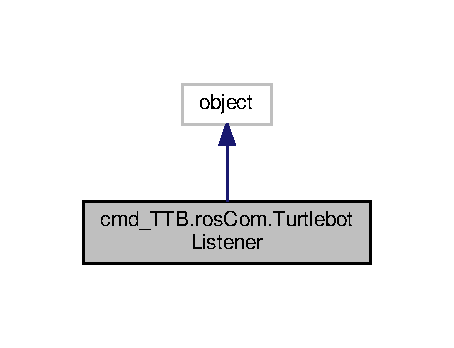
\includegraphics[width=218pt]{classcmd__TTB_1_1rosCom_1_1TurtlebotListener__inherit__graph}
\end{center}
\end{figure}


Collaboration diagram for cmd\+\_\+\+T\+T\+B.\+ros\+Com.\+Turtlebot\+Listener\+:\nopagebreak
\begin{figure}[H]
\begin{center}
\leavevmode
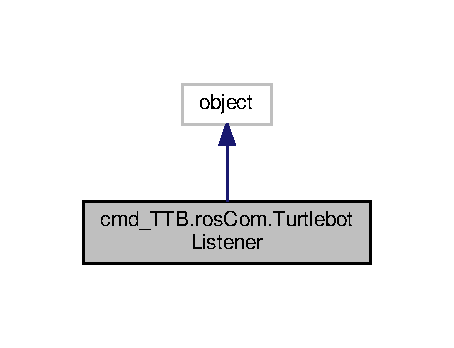
\includegraphics[width=218pt]{classcmd__TTB_1_1rosCom_1_1TurtlebotListener__coll__graph}
\end{center}
\end{figure}
\subsection*{Public Member Functions}
\begin{DoxyCompactItemize}
\item 
def \hyperlink{classcmd__TTB_1_1rosCom_1_1TurtlebotListener_aa8320dde62def929f13c1989cda19b47}{\+\_\+\+\_\+init\+\_\+\+\_\+} (self, \hyperlink{classcmd__TTB_1_1rosCom_1_1TurtlebotListener_ad2568a558e1f8eb925e740feecd64da8}{topic}=\char`\"{}/odom\char`\"{}, F\+R\+E\+Q\+U\+E\+N\+CE=10)
\item 
def \hyperlink{classcmd__TTB_1_1rosCom_1_1TurtlebotListener_a597fc8de6590574505b032bc6ad0cdca}{kill} (self)
\item 
def \hyperlink{classcmd__TTB_1_1rosCom_1_1TurtlebotListener_a25ae5c5eacd3aa023aadcec9807b9e17}{init\+Nodes} (self)
\item 
def \hyperlink{classcmd__TTB_1_1rosCom_1_1TurtlebotListener_a2b85e835bd92eb645e96fca1086ea457}{reset\+Odom} (self)
\item 
def \hyperlink{classcmd__TTB_1_1rosCom_1_1TurtlebotListener_a4ee11b98fcffb76eb92865ba8d3f9ede}{callback} (self, data)
\item 
def \hyperlink{classcmd__TTB_1_1rosCom_1_1TurtlebotListener_a6bf38ca3f7ce77d48989eca2b1ae342c}{get\+X\+Y\+Theta} (self)
\item 
def \hyperlink{classcmd__TTB_1_1rosCom_1_1TurtlebotListener_a15c2ab52985c74917e81e3309ba53dce}{get\+VW} (self)
\item 
def \hyperlink{classcmd__TTB_1_1rosCom_1_1TurtlebotListener_ab9e1187d6fbb94c299af17c1834bd5fc}{get\+A\+Mean\+Of\+X\+Y\+Theta} (self)
\end{DoxyCompactItemize}
\subsection*{Public Attributes}
\begin{DoxyCompactItemize}
\item 
\hyperlink{classcmd__TTB_1_1rosCom_1_1TurtlebotListener_a151f0bbf98f037cfbb7d4f37f24a41ce}{frequence}
\item 
\hyperlink{classcmd__TTB_1_1rosCom_1_1TurtlebotListener_a1b553612cfd5f7a036135d9d1ea6c8d4}{thread}
\item 
\hyperlink{classcmd__TTB_1_1rosCom_1_1TurtlebotListener_a38b4dd694dcbe7b0130c14b7c0d4258f}{lock}
\item 
\hyperlink{classcmd__TTB_1_1rosCom_1_1TurtlebotListener_a239216e633677cdfa9454413d5d25b7a}{theta\+Lifter}
\item 
\hyperlink{classcmd__TTB_1_1rosCom_1_1TurtlebotListener_a0f4a3af5847d9cc7286df47ff9c210ba}{x}
\item 
\hyperlink{classcmd__TTB_1_1rosCom_1_1TurtlebotListener_a2a84aa6fb1fa37ed9ebe192453595ee3}{theta}
\item 
\hyperlink{classcmd__TTB_1_1rosCom_1_1TurtlebotListener_a95654744b7edf1026dd83eb188362a16}{q1}
\item 
\hyperlink{classcmd__TTB_1_1rosCom_1_1TurtlebotListener_aaa33f36155d66b69c8ee6c42d3e41653}{q2}
\item 
\hyperlink{classcmd__TTB_1_1rosCom_1_1TurtlebotListener_a990048a7622c36d60e21db4095824da1}{q3}
\item 
\hyperlink{classcmd__TTB_1_1rosCom_1_1TurtlebotListener_a746a7fb8e2d8d8f36d450eed84f883c3}{q4}
\item 
\hyperlink{classcmd__TTB_1_1rosCom_1_1TurtlebotListener_a65dcdf893e0634569fb6ef82ee2b994b}{y}
\item 
\hyperlink{classcmd__TTB_1_1rosCom_1_1TurtlebotListener_ae4e7da79789355f09d2160df1a1a70e9}{v}
\item 
\hyperlink{classcmd__TTB_1_1rosCom_1_1TurtlebotListener_a42be0d63f609e68b70a368f6abfcf51c}{w}
\item 
\hyperlink{classcmd__TTB_1_1rosCom_1_1TurtlebotListener_ad2568a558e1f8eb925e740feecd64da8}{topic}
\item 
\hyperlink{classcmd__TTB_1_1rosCom_1_1TurtlebotListener_a0cc23ef555157723d4134bb26d4eb688}{rate}
\item 
\hyperlink{classcmd__TTB_1_1rosCom_1_1TurtlebotListener_ac7f613cf46497b805eb2c98a4d0b9140}{p}
\end{DoxyCompactItemize}


\subsection{Constructor \& Destructor Documentation}
\index{cmd\+\_\+\+T\+T\+B\+::ros\+Com\+::\+Turtlebot\+Listener@{cmd\+\_\+\+T\+T\+B\+::ros\+Com\+::\+Turtlebot\+Listener}!\+\_\+\+\_\+init\+\_\+\+\_\+@{\+\_\+\+\_\+init\+\_\+\+\_\+}}
\index{\+\_\+\+\_\+init\+\_\+\+\_\+@{\+\_\+\+\_\+init\+\_\+\+\_\+}!cmd\+\_\+\+T\+T\+B\+::ros\+Com\+::\+Turtlebot\+Listener@{cmd\+\_\+\+T\+T\+B\+::ros\+Com\+::\+Turtlebot\+Listener}}
\subsubsection[{\texorpdfstring{\+\_\+\+\_\+init\+\_\+\+\_\+(self, topic=""/odom"", F\+R\+E\+Q\+U\+E\+N\+C\+E=10)}{__init__(self, topic="/odom", FREQUENCE=10)}}]{\setlength{\rightskip}{0pt plus 5cm}def cmd\+\_\+\+T\+T\+B.\+ros\+Com.\+Turtlebot\+Listener.\+\_\+\+\_\+init\+\_\+\+\_\+ (
\begin{DoxyParamCaption}
\item[{}]{self, }
\item[{}]{topic = {\ttfamily \char`\"{}/odom\char`\"{}}, }
\item[{}]{F\+R\+E\+Q\+U\+E\+N\+CE = {\ttfamily 10}}
\end{DoxyParamCaption}
)}\hypertarget{classcmd__TTB_1_1rosCom_1_1TurtlebotListener_aa8320dde62def929f13c1989cda19b47}{}\label{classcmd__TTB_1_1rosCom_1_1TurtlebotListener_aa8320dde62def929f13c1989cda19b47}


\subsection{Member Function Documentation}
\index{cmd\+\_\+\+T\+T\+B\+::ros\+Com\+::\+Turtlebot\+Listener@{cmd\+\_\+\+T\+T\+B\+::ros\+Com\+::\+Turtlebot\+Listener}!callback@{callback}}
\index{callback@{callback}!cmd\+\_\+\+T\+T\+B\+::ros\+Com\+::\+Turtlebot\+Listener@{cmd\+\_\+\+T\+T\+B\+::ros\+Com\+::\+Turtlebot\+Listener}}
\subsubsection[{\texorpdfstring{callback(self, data)}{callback(self, data)}}]{\setlength{\rightskip}{0pt plus 5cm}def cmd\+\_\+\+T\+T\+B.\+ros\+Com.\+Turtlebot\+Listener.\+callback (
\begin{DoxyParamCaption}
\item[{}]{self, }
\item[{}]{data}
\end{DoxyParamCaption}
)}\hypertarget{classcmd__TTB_1_1rosCom_1_1TurtlebotListener_a4ee11b98fcffb76eb92865ba8d3f9ede}{}\label{classcmd__TTB_1_1rosCom_1_1TurtlebotListener_a4ee11b98fcffb76eb92865ba8d3f9ede}
\begin{DoxyVerb}Fonction executee a chaque fois qu'une valeur est disponible dans le topic\end{DoxyVerb}
 \index{cmd\+\_\+\+T\+T\+B\+::ros\+Com\+::\+Turtlebot\+Listener@{cmd\+\_\+\+T\+T\+B\+::ros\+Com\+::\+Turtlebot\+Listener}!get\+A\+Mean\+Of\+X\+Y\+Theta@{get\+A\+Mean\+Of\+X\+Y\+Theta}}
\index{get\+A\+Mean\+Of\+X\+Y\+Theta@{get\+A\+Mean\+Of\+X\+Y\+Theta}!cmd\+\_\+\+T\+T\+B\+::ros\+Com\+::\+Turtlebot\+Listener@{cmd\+\_\+\+T\+T\+B\+::ros\+Com\+::\+Turtlebot\+Listener}}
\subsubsection[{\texorpdfstring{get\+A\+Mean\+Of\+X\+Y\+Theta(self)}{getAMeanOfXYTheta(self)}}]{\setlength{\rightskip}{0pt plus 5cm}def cmd\+\_\+\+T\+T\+B.\+ros\+Com.\+Turtlebot\+Listener.\+get\+A\+Mean\+Of\+X\+Y\+Theta (
\begin{DoxyParamCaption}
\item[{}]{self}
\end{DoxyParamCaption}
)}\hypertarget{classcmd__TTB_1_1rosCom_1_1TurtlebotListener_ab9e1187d6fbb94c299af17c1834bd5fc}{}\label{classcmd__TTB_1_1rosCom_1_1TurtlebotListener_ab9e1187d6fbb94c299af17c1834bd5fc}
\begin{DoxyVerb}Retourne une valeur moyenne de x,y,theta sur une seconde\end{DoxyVerb}
 \index{cmd\+\_\+\+T\+T\+B\+::ros\+Com\+::\+Turtlebot\+Listener@{cmd\+\_\+\+T\+T\+B\+::ros\+Com\+::\+Turtlebot\+Listener}!get\+VW@{get\+VW}}
\index{get\+VW@{get\+VW}!cmd\+\_\+\+T\+T\+B\+::ros\+Com\+::\+Turtlebot\+Listener@{cmd\+\_\+\+T\+T\+B\+::ros\+Com\+::\+Turtlebot\+Listener}}
\subsubsection[{\texorpdfstring{get\+V\+W(self)}{getVW(self)}}]{\setlength{\rightskip}{0pt plus 5cm}def cmd\+\_\+\+T\+T\+B.\+ros\+Com.\+Turtlebot\+Listener.\+get\+VW (
\begin{DoxyParamCaption}
\item[{}]{self}
\end{DoxyParamCaption}
)}\hypertarget{classcmd__TTB_1_1rosCom_1_1TurtlebotListener_a15c2ab52985c74917e81e3309ba53dce}{}\label{classcmd__TTB_1_1rosCom_1_1TurtlebotListener_a15c2ab52985c74917e81e3309ba53dce}
\begin{DoxyVerb}Retourne v et w\end{DoxyVerb}
 \index{cmd\+\_\+\+T\+T\+B\+::ros\+Com\+::\+Turtlebot\+Listener@{cmd\+\_\+\+T\+T\+B\+::ros\+Com\+::\+Turtlebot\+Listener}!get\+X\+Y\+Theta@{get\+X\+Y\+Theta}}
\index{get\+X\+Y\+Theta@{get\+X\+Y\+Theta}!cmd\+\_\+\+T\+T\+B\+::ros\+Com\+::\+Turtlebot\+Listener@{cmd\+\_\+\+T\+T\+B\+::ros\+Com\+::\+Turtlebot\+Listener}}
\subsubsection[{\texorpdfstring{get\+X\+Y\+Theta(self)}{getXYTheta(self)}}]{\setlength{\rightskip}{0pt plus 5cm}def cmd\+\_\+\+T\+T\+B.\+ros\+Com.\+Turtlebot\+Listener.\+get\+X\+Y\+Theta (
\begin{DoxyParamCaption}
\item[{}]{self}
\end{DoxyParamCaption}
)}\hypertarget{classcmd__TTB_1_1rosCom_1_1TurtlebotListener_a6bf38ca3f7ce77d48989eca2b1ae342c}{}\label{classcmd__TTB_1_1rosCom_1_1TurtlebotListener_a6bf38ca3f7ce77d48989eca2b1ae342c}
\begin{DoxyVerb}Retourne x,y,theta\end{DoxyVerb}
 \index{cmd\+\_\+\+T\+T\+B\+::ros\+Com\+::\+Turtlebot\+Listener@{cmd\+\_\+\+T\+T\+B\+::ros\+Com\+::\+Turtlebot\+Listener}!init\+Nodes@{init\+Nodes}}
\index{init\+Nodes@{init\+Nodes}!cmd\+\_\+\+T\+T\+B\+::ros\+Com\+::\+Turtlebot\+Listener@{cmd\+\_\+\+T\+T\+B\+::ros\+Com\+::\+Turtlebot\+Listener}}
\subsubsection[{\texorpdfstring{init\+Nodes(self)}{initNodes(self)}}]{\setlength{\rightskip}{0pt plus 5cm}def cmd\+\_\+\+T\+T\+B.\+ros\+Com.\+Turtlebot\+Listener.\+init\+Nodes (
\begin{DoxyParamCaption}
\item[{}]{self}
\end{DoxyParamCaption}
)}\hypertarget{classcmd__TTB_1_1rosCom_1_1TurtlebotListener_a25ae5c5eacd3aa023aadcec9807b9e17}{}\label{classcmd__TTB_1_1rosCom_1_1TurtlebotListener_a25ae5c5eacd3aa023aadcec9807b9e17}
\begin{DoxyVerb}(Fonction interne/devrait etre declaree prive) empeche le node de se fermer et execute les callbacks en arriere plan\end{DoxyVerb}
 \index{cmd\+\_\+\+T\+T\+B\+::ros\+Com\+::\+Turtlebot\+Listener@{cmd\+\_\+\+T\+T\+B\+::ros\+Com\+::\+Turtlebot\+Listener}!kill@{kill}}
\index{kill@{kill}!cmd\+\_\+\+T\+T\+B\+::ros\+Com\+::\+Turtlebot\+Listener@{cmd\+\_\+\+T\+T\+B\+::ros\+Com\+::\+Turtlebot\+Listener}}
\subsubsection[{\texorpdfstring{kill(self)}{kill(self)}}]{\setlength{\rightskip}{0pt plus 5cm}def cmd\+\_\+\+T\+T\+B.\+ros\+Com.\+Turtlebot\+Listener.\+kill (
\begin{DoxyParamCaption}
\item[{}]{self}
\end{DoxyParamCaption}
)}\hypertarget{classcmd__TTB_1_1rosCom_1_1TurtlebotListener_a597fc8de6590574505b032bc6ad0cdca}{}\label{classcmd__TTB_1_1rosCom_1_1TurtlebotListener_a597fc8de6590574505b032bc6ad0cdca}
\begin{DoxyVerb}Doit etre appelée en fin de script si un listener a ete cree\end{DoxyVerb}
 \index{cmd\+\_\+\+T\+T\+B\+::ros\+Com\+::\+Turtlebot\+Listener@{cmd\+\_\+\+T\+T\+B\+::ros\+Com\+::\+Turtlebot\+Listener}!reset\+Odom@{reset\+Odom}}
\index{reset\+Odom@{reset\+Odom}!cmd\+\_\+\+T\+T\+B\+::ros\+Com\+::\+Turtlebot\+Listener@{cmd\+\_\+\+T\+T\+B\+::ros\+Com\+::\+Turtlebot\+Listener}}
\subsubsection[{\texorpdfstring{reset\+Odom(self)}{resetOdom(self)}}]{\setlength{\rightskip}{0pt plus 5cm}def cmd\+\_\+\+T\+T\+B.\+ros\+Com.\+Turtlebot\+Listener.\+reset\+Odom (
\begin{DoxyParamCaption}
\item[{}]{self}
\end{DoxyParamCaption}
)}\hypertarget{classcmd__TTB_1_1rosCom_1_1TurtlebotListener_a2b85e835bd92eb645e96fca1086ea457}{}\label{classcmd__TTB_1_1rosCom_1_1TurtlebotListener_a2b85e835bd92eb645e96fca1086ea457}
\begin{DoxyVerb}reset l'odometrie du TTB\end{DoxyVerb}
 

\subsection{Member Data Documentation}
\index{cmd\+\_\+\+T\+T\+B\+::ros\+Com\+::\+Turtlebot\+Listener@{cmd\+\_\+\+T\+T\+B\+::ros\+Com\+::\+Turtlebot\+Listener}!frequence@{frequence}}
\index{frequence@{frequence}!cmd\+\_\+\+T\+T\+B\+::ros\+Com\+::\+Turtlebot\+Listener@{cmd\+\_\+\+T\+T\+B\+::ros\+Com\+::\+Turtlebot\+Listener}}
\subsubsection[{\texorpdfstring{frequence}{frequence}}]{\setlength{\rightskip}{0pt plus 5cm}cmd\+\_\+\+T\+T\+B.\+ros\+Com.\+Turtlebot\+Listener.\+frequence}\hypertarget{classcmd__TTB_1_1rosCom_1_1TurtlebotListener_a151f0bbf98f037cfbb7d4f37f24a41ce}{}\label{classcmd__TTB_1_1rosCom_1_1TurtlebotListener_a151f0bbf98f037cfbb7d4f37f24a41ce}
\index{cmd\+\_\+\+T\+T\+B\+::ros\+Com\+::\+Turtlebot\+Listener@{cmd\+\_\+\+T\+T\+B\+::ros\+Com\+::\+Turtlebot\+Listener}!lock@{lock}}
\index{lock@{lock}!cmd\+\_\+\+T\+T\+B\+::ros\+Com\+::\+Turtlebot\+Listener@{cmd\+\_\+\+T\+T\+B\+::ros\+Com\+::\+Turtlebot\+Listener}}
\subsubsection[{\texorpdfstring{lock}{lock}}]{\setlength{\rightskip}{0pt plus 5cm}cmd\+\_\+\+T\+T\+B.\+ros\+Com.\+Turtlebot\+Listener.\+lock}\hypertarget{classcmd__TTB_1_1rosCom_1_1TurtlebotListener_a38b4dd694dcbe7b0130c14b7c0d4258f}{}\label{classcmd__TTB_1_1rosCom_1_1TurtlebotListener_a38b4dd694dcbe7b0130c14b7c0d4258f}
\index{cmd\+\_\+\+T\+T\+B\+::ros\+Com\+::\+Turtlebot\+Listener@{cmd\+\_\+\+T\+T\+B\+::ros\+Com\+::\+Turtlebot\+Listener}!p@{p}}
\index{p@{p}!cmd\+\_\+\+T\+T\+B\+::ros\+Com\+::\+Turtlebot\+Listener@{cmd\+\_\+\+T\+T\+B\+::ros\+Com\+::\+Turtlebot\+Listener}}
\subsubsection[{\texorpdfstring{p}{p}}]{\setlength{\rightskip}{0pt plus 5cm}cmd\+\_\+\+T\+T\+B.\+ros\+Com.\+Turtlebot\+Listener.\+p}\hypertarget{classcmd__TTB_1_1rosCom_1_1TurtlebotListener_ac7f613cf46497b805eb2c98a4d0b9140}{}\label{classcmd__TTB_1_1rosCom_1_1TurtlebotListener_ac7f613cf46497b805eb2c98a4d0b9140}
\index{cmd\+\_\+\+T\+T\+B\+::ros\+Com\+::\+Turtlebot\+Listener@{cmd\+\_\+\+T\+T\+B\+::ros\+Com\+::\+Turtlebot\+Listener}!q1@{q1}}
\index{q1@{q1}!cmd\+\_\+\+T\+T\+B\+::ros\+Com\+::\+Turtlebot\+Listener@{cmd\+\_\+\+T\+T\+B\+::ros\+Com\+::\+Turtlebot\+Listener}}
\subsubsection[{\texorpdfstring{q1}{q1}}]{\setlength{\rightskip}{0pt plus 5cm}cmd\+\_\+\+T\+T\+B.\+ros\+Com.\+Turtlebot\+Listener.\+q1}\hypertarget{classcmd__TTB_1_1rosCom_1_1TurtlebotListener_a95654744b7edf1026dd83eb188362a16}{}\label{classcmd__TTB_1_1rosCom_1_1TurtlebotListener_a95654744b7edf1026dd83eb188362a16}
\index{cmd\+\_\+\+T\+T\+B\+::ros\+Com\+::\+Turtlebot\+Listener@{cmd\+\_\+\+T\+T\+B\+::ros\+Com\+::\+Turtlebot\+Listener}!q2@{q2}}
\index{q2@{q2}!cmd\+\_\+\+T\+T\+B\+::ros\+Com\+::\+Turtlebot\+Listener@{cmd\+\_\+\+T\+T\+B\+::ros\+Com\+::\+Turtlebot\+Listener}}
\subsubsection[{\texorpdfstring{q2}{q2}}]{\setlength{\rightskip}{0pt plus 5cm}cmd\+\_\+\+T\+T\+B.\+ros\+Com.\+Turtlebot\+Listener.\+q2}\hypertarget{classcmd__TTB_1_1rosCom_1_1TurtlebotListener_aaa33f36155d66b69c8ee6c42d3e41653}{}\label{classcmd__TTB_1_1rosCom_1_1TurtlebotListener_aaa33f36155d66b69c8ee6c42d3e41653}
\index{cmd\+\_\+\+T\+T\+B\+::ros\+Com\+::\+Turtlebot\+Listener@{cmd\+\_\+\+T\+T\+B\+::ros\+Com\+::\+Turtlebot\+Listener}!q3@{q3}}
\index{q3@{q3}!cmd\+\_\+\+T\+T\+B\+::ros\+Com\+::\+Turtlebot\+Listener@{cmd\+\_\+\+T\+T\+B\+::ros\+Com\+::\+Turtlebot\+Listener}}
\subsubsection[{\texorpdfstring{q3}{q3}}]{\setlength{\rightskip}{0pt plus 5cm}cmd\+\_\+\+T\+T\+B.\+ros\+Com.\+Turtlebot\+Listener.\+q3}\hypertarget{classcmd__TTB_1_1rosCom_1_1TurtlebotListener_a990048a7622c36d60e21db4095824da1}{}\label{classcmd__TTB_1_1rosCom_1_1TurtlebotListener_a990048a7622c36d60e21db4095824da1}
\index{cmd\+\_\+\+T\+T\+B\+::ros\+Com\+::\+Turtlebot\+Listener@{cmd\+\_\+\+T\+T\+B\+::ros\+Com\+::\+Turtlebot\+Listener}!q4@{q4}}
\index{q4@{q4}!cmd\+\_\+\+T\+T\+B\+::ros\+Com\+::\+Turtlebot\+Listener@{cmd\+\_\+\+T\+T\+B\+::ros\+Com\+::\+Turtlebot\+Listener}}
\subsubsection[{\texorpdfstring{q4}{q4}}]{\setlength{\rightskip}{0pt plus 5cm}cmd\+\_\+\+T\+T\+B.\+ros\+Com.\+Turtlebot\+Listener.\+q4}\hypertarget{classcmd__TTB_1_1rosCom_1_1TurtlebotListener_a746a7fb8e2d8d8f36d450eed84f883c3}{}\label{classcmd__TTB_1_1rosCom_1_1TurtlebotListener_a746a7fb8e2d8d8f36d450eed84f883c3}
\index{cmd\+\_\+\+T\+T\+B\+::ros\+Com\+::\+Turtlebot\+Listener@{cmd\+\_\+\+T\+T\+B\+::ros\+Com\+::\+Turtlebot\+Listener}!rate@{rate}}
\index{rate@{rate}!cmd\+\_\+\+T\+T\+B\+::ros\+Com\+::\+Turtlebot\+Listener@{cmd\+\_\+\+T\+T\+B\+::ros\+Com\+::\+Turtlebot\+Listener}}
\subsubsection[{\texorpdfstring{rate}{rate}}]{\setlength{\rightskip}{0pt plus 5cm}cmd\+\_\+\+T\+T\+B.\+ros\+Com.\+Turtlebot\+Listener.\+rate}\hypertarget{classcmd__TTB_1_1rosCom_1_1TurtlebotListener_a0cc23ef555157723d4134bb26d4eb688}{}\label{classcmd__TTB_1_1rosCom_1_1TurtlebotListener_a0cc23ef555157723d4134bb26d4eb688}
\index{cmd\+\_\+\+T\+T\+B\+::ros\+Com\+::\+Turtlebot\+Listener@{cmd\+\_\+\+T\+T\+B\+::ros\+Com\+::\+Turtlebot\+Listener}!theta@{theta}}
\index{theta@{theta}!cmd\+\_\+\+T\+T\+B\+::ros\+Com\+::\+Turtlebot\+Listener@{cmd\+\_\+\+T\+T\+B\+::ros\+Com\+::\+Turtlebot\+Listener}}
\subsubsection[{\texorpdfstring{theta}{theta}}]{\setlength{\rightskip}{0pt plus 5cm}cmd\+\_\+\+T\+T\+B.\+ros\+Com.\+Turtlebot\+Listener.\+theta}\hypertarget{classcmd__TTB_1_1rosCom_1_1TurtlebotListener_a2a84aa6fb1fa37ed9ebe192453595ee3}{}\label{classcmd__TTB_1_1rosCom_1_1TurtlebotListener_a2a84aa6fb1fa37ed9ebe192453595ee3}
\index{cmd\+\_\+\+T\+T\+B\+::ros\+Com\+::\+Turtlebot\+Listener@{cmd\+\_\+\+T\+T\+B\+::ros\+Com\+::\+Turtlebot\+Listener}!theta\+Lifter@{theta\+Lifter}}
\index{theta\+Lifter@{theta\+Lifter}!cmd\+\_\+\+T\+T\+B\+::ros\+Com\+::\+Turtlebot\+Listener@{cmd\+\_\+\+T\+T\+B\+::ros\+Com\+::\+Turtlebot\+Listener}}
\subsubsection[{\texorpdfstring{theta\+Lifter}{thetaLifter}}]{\setlength{\rightskip}{0pt plus 5cm}cmd\+\_\+\+T\+T\+B.\+ros\+Com.\+Turtlebot\+Listener.\+theta\+Lifter}\hypertarget{classcmd__TTB_1_1rosCom_1_1TurtlebotListener_a239216e633677cdfa9454413d5d25b7a}{}\label{classcmd__TTB_1_1rosCom_1_1TurtlebotListener_a239216e633677cdfa9454413d5d25b7a}
\index{cmd\+\_\+\+T\+T\+B\+::ros\+Com\+::\+Turtlebot\+Listener@{cmd\+\_\+\+T\+T\+B\+::ros\+Com\+::\+Turtlebot\+Listener}!thread@{thread}}
\index{thread@{thread}!cmd\+\_\+\+T\+T\+B\+::ros\+Com\+::\+Turtlebot\+Listener@{cmd\+\_\+\+T\+T\+B\+::ros\+Com\+::\+Turtlebot\+Listener}}
\subsubsection[{\texorpdfstring{thread}{thread}}]{\setlength{\rightskip}{0pt plus 5cm}cmd\+\_\+\+T\+T\+B.\+ros\+Com.\+Turtlebot\+Listener.\+thread}\hypertarget{classcmd__TTB_1_1rosCom_1_1TurtlebotListener_a1b553612cfd5f7a036135d9d1ea6c8d4}{}\label{classcmd__TTB_1_1rosCom_1_1TurtlebotListener_a1b553612cfd5f7a036135d9d1ea6c8d4}
\index{cmd\+\_\+\+T\+T\+B\+::ros\+Com\+::\+Turtlebot\+Listener@{cmd\+\_\+\+T\+T\+B\+::ros\+Com\+::\+Turtlebot\+Listener}!topic@{topic}}
\index{topic@{topic}!cmd\+\_\+\+T\+T\+B\+::ros\+Com\+::\+Turtlebot\+Listener@{cmd\+\_\+\+T\+T\+B\+::ros\+Com\+::\+Turtlebot\+Listener}}
\subsubsection[{\texorpdfstring{topic}{topic}}]{\setlength{\rightskip}{0pt plus 5cm}cmd\+\_\+\+T\+T\+B.\+ros\+Com.\+Turtlebot\+Listener.\+topic}\hypertarget{classcmd__TTB_1_1rosCom_1_1TurtlebotListener_ad2568a558e1f8eb925e740feecd64da8}{}\label{classcmd__TTB_1_1rosCom_1_1TurtlebotListener_ad2568a558e1f8eb925e740feecd64da8}
\index{cmd\+\_\+\+T\+T\+B\+::ros\+Com\+::\+Turtlebot\+Listener@{cmd\+\_\+\+T\+T\+B\+::ros\+Com\+::\+Turtlebot\+Listener}!v@{v}}
\index{v@{v}!cmd\+\_\+\+T\+T\+B\+::ros\+Com\+::\+Turtlebot\+Listener@{cmd\+\_\+\+T\+T\+B\+::ros\+Com\+::\+Turtlebot\+Listener}}
\subsubsection[{\texorpdfstring{v}{v}}]{\setlength{\rightskip}{0pt plus 5cm}cmd\+\_\+\+T\+T\+B.\+ros\+Com.\+Turtlebot\+Listener.\+v}\hypertarget{classcmd__TTB_1_1rosCom_1_1TurtlebotListener_ae4e7da79789355f09d2160df1a1a70e9}{}\label{classcmd__TTB_1_1rosCom_1_1TurtlebotListener_ae4e7da79789355f09d2160df1a1a70e9}
\index{cmd\+\_\+\+T\+T\+B\+::ros\+Com\+::\+Turtlebot\+Listener@{cmd\+\_\+\+T\+T\+B\+::ros\+Com\+::\+Turtlebot\+Listener}!w@{w}}
\index{w@{w}!cmd\+\_\+\+T\+T\+B\+::ros\+Com\+::\+Turtlebot\+Listener@{cmd\+\_\+\+T\+T\+B\+::ros\+Com\+::\+Turtlebot\+Listener}}
\subsubsection[{\texorpdfstring{w}{w}}]{\setlength{\rightskip}{0pt plus 5cm}cmd\+\_\+\+T\+T\+B.\+ros\+Com.\+Turtlebot\+Listener.\+w}\hypertarget{classcmd__TTB_1_1rosCom_1_1TurtlebotListener_a42be0d63f609e68b70a368f6abfcf51c}{}\label{classcmd__TTB_1_1rosCom_1_1TurtlebotListener_a42be0d63f609e68b70a368f6abfcf51c}
\index{cmd\+\_\+\+T\+T\+B\+::ros\+Com\+::\+Turtlebot\+Listener@{cmd\+\_\+\+T\+T\+B\+::ros\+Com\+::\+Turtlebot\+Listener}!x@{x}}
\index{x@{x}!cmd\+\_\+\+T\+T\+B\+::ros\+Com\+::\+Turtlebot\+Listener@{cmd\+\_\+\+T\+T\+B\+::ros\+Com\+::\+Turtlebot\+Listener}}
\subsubsection[{\texorpdfstring{x}{x}}]{\setlength{\rightskip}{0pt plus 5cm}cmd\+\_\+\+T\+T\+B.\+ros\+Com.\+Turtlebot\+Listener.\+x}\hypertarget{classcmd__TTB_1_1rosCom_1_1TurtlebotListener_a0f4a3af5847d9cc7286df47ff9c210ba}{}\label{classcmd__TTB_1_1rosCom_1_1TurtlebotListener_a0f4a3af5847d9cc7286df47ff9c210ba}
\index{cmd\+\_\+\+T\+T\+B\+::ros\+Com\+::\+Turtlebot\+Listener@{cmd\+\_\+\+T\+T\+B\+::ros\+Com\+::\+Turtlebot\+Listener}!y@{y}}
\index{y@{y}!cmd\+\_\+\+T\+T\+B\+::ros\+Com\+::\+Turtlebot\+Listener@{cmd\+\_\+\+T\+T\+B\+::ros\+Com\+::\+Turtlebot\+Listener}}
\subsubsection[{\texorpdfstring{y}{y}}]{\setlength{\rightskip}{0pt plus 5cm}cmd\+\_\+\+T\+T\+B.\+ros\+Com.\+Turtlebot\+Listener.\+y}\hypertarget{classcmd__TTB_1_1rosCom_1_1TurtlebotListener_a65dcdf893e0634569fb6ef82ee2b994b}{}\label{classcmd__TTB_1_1rosCom_1_1TurtlebotListener_a65dcdf893e0634569fb6ef82ee2b994b}


The documentation for this class was generated from the following file\+:\begin{DoxyCompactItemize}
\item 
\hyperlink{rosCom_8py}{ros\+Com.\+py}\end{DoxyCompactItemize}

\hypertarget{classcmd__TTB_1_1controllers_1_1turtlebotPID}{}\section{cmd\+\_\+\+T\+T\+B.\+controllers.\+turtlebot\+P\+ID Class Reference}
\label{classcmd__TTB_1_1controllers_1_1turtlebotPID}\index{cmd\+\_\+\+T\+T\+B.\+controllers.\+turtlebot\+P\+ID@{cmd\+\_\+\+T\+T\+B.\+controllers.\+turtlebot\+P\+ID}}


Inheritance diagram for cmd\+\_\+\+T\+T\+B.\+controllers.\+turtlebot\+P\+ID\+:\nopagebreak
\begin{figure}[H]
\begin{center}
\leavevmode
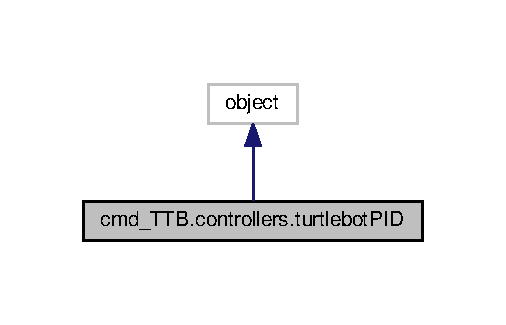
\includegraphics[width=243pt]{classcmd__TTB_1_1controllers_1_1turtlebotPID__inherit__graph}
\end{center}
\end{figure}


Collaboration diagram for cmd\+\_\+\+T\+T\+B.\+controllers.\+turtlebot\+P\+ID\+:\nopagebreak
\begin{figure}[H]
\begin{center}
\leavevmode
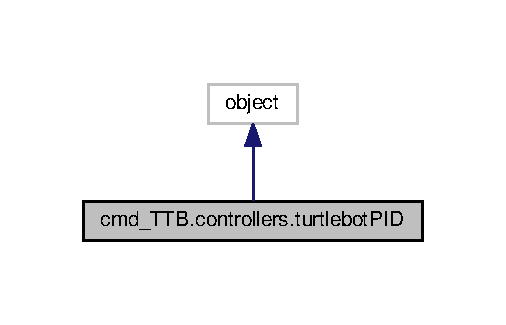
\includegraphics[width=243pt]{classcmd__TTB_1_1controllers_1_1turtlebotPID__coll__graph}
\end{center}
\end{figure}
\subsection*{Public Member Functions}
\begin{DoxyCompactItemize}
\item 
def \hyperlink{classcmd__TTB_1_1controllers_1_1turtlebotPID_a3360909164559c841e600896014a60b4}{\+\_\+\+\_\+init\+\_\+\+\_\+} (self, \hyperlink{classcmd__TTB_1_1controllers_1_1turtlebotPID_a46f9e76ece4ade360926bdc5250cdfc3}{kp}, \hyperlink{classcmd__TTB_1_1controllers_1_1turtlebotPID_aaf815b510701e946034699cf9039b961}{ki}, \hyperlink{classcmd__TTB_1_1controllers_1_1turtlebotPID_a33fb24bec3035fd064ce48c58420fde8}{kd}, \hyperlink{classcmd__TTB_1_1controllers_1_1turtlebotPID_ab20832f88555ed864be4e1f3f37ce2d7}{F\+R\+EQ}, \hyperlink{classcmd__TTB_1_1controllers_1_1turtlebotPID_a9eedbb29702ca64a002d8b13a79f515b}{u\+Max}=1)
\item 
def \hyperlink{classcmd__TTB_1_1controllers_1_1turtlebotPID_acfb641d74e87200c6a6832bfb22de252}{getU} (self, \hyperlink{classcmd__TTB_1_1controllers_1_1turtlebotPID_ac4c729835bb914598eefd16a3278ce14}{e})
\begin{DoxyCompactList}\small\item\em Computes the new control state u=(v,w) from the raw one e. \end{DoxyCompactList}\item 
def \hyperlink{classcmd__TTB_1_1controllers_1_1turtlebotPID_a9a16fe7aab46c6cbc8e31ee505d780d9}{Add\+U\+To\+The\+List} (self, Output)
\item 
def \hyperlink{classcmd__TTB_1_1controllers_1_1turtlebotPID_adf5ae9d1784ea20c14c626039b4e5136}{Add\+R\+To\+The\+List} (self, Input)
\item 
def \hyperlink{classcmd__TTB_1_1controllers_1_1turtlebotPID_aae3de1d737681be0f420a3ed8f2b63e8}{Output\+Saturation} (self, u)
\end{DoxyCompactItemize}
\subsection*{Public Attributes}
\begin{DoxyCompactItemize}
\item 
\hyperlink{classcmd__TTB_1_1controllers_1_1turtlebotPID_a9eedbb29702ca64a002d8b13a79f515b}{u\+Max}
\item 
\hyperlink{classcmd__TTB_1_1controllers_1_1turtlebotPID_a46f9e76ece4ade360926bdc5250cdfc3}{kp}
\item 
\hyperlink{classcmd__TTB_1_1controllers_1_1turtlebotPID_aaf815b510701e946034699cf9039b961}{ki}
\item 
\hyperlink{classcmd__TTB_1_1controllers_1_1turtlebotPID_a33fb24bec3035fd064ce48c58420fde8}{kd}
\item 
\hyperlink{classcmd__TTB_1_1controllers_1_1turtlebotPID_ab20832f88555ed864be4e1f3f37ce2d7}{F\+R\+EQ}
\item 
\hyperlink{classcmd__TTB_1_1controllers_1_1turtlebotPID_abc36f71fca7350bacae66d199d9cc18f}{U}
\item 
\hyperlink{classcmd__TTB_1_1controllers_1_1turtlebotPID_ac4c729835bb914598eefd16a3278ce14}{e}
\end{DoxyCompactItemize}


\subsection{Constructor \& Destructor Documentation}
\index{cmd\+\_\+\+T\+T\+B\+::controllers\+::turtlebot\+P\+ID@{cmd\+\_\+\+T\+T\+B\+::controllers\+::turtlebot\+P\+ID}!\+\_\+\+\_\+init\+\_\+\+\_\+@{\+\_\+\+\_\+init\+\_\+\+\_\+}}
\index{\+\_\+\+\_\+init\+\_\+\+\_\+@{\+\_\+\+\_\+init\+\_\+\+\_\+}!cmd\+\_\+\+T\+T\+B\+::controllers\+::turtlebot\+P\+ID@{cmd\+\_\+\+T\+T\+B\+::controllers\+::turtlebot\+P\+ID}}
\subsubsection[{\texorpdfstring{\+\_\+\+\_\+init\+\_\+\+\_\+(self, kp, ki, kd, F\+R\+E\+Q, u\+Max=1)}{__init__(self, kp, ki, kd, FREQ, uMax=1)}}]{\setlength{\rightskip}{0pt plus 5cm}def cmd\+\_\+\+T\+T\+B.\+controllers.\+turtlebot\+P\+I\+D.\+\_\+\+\_\+init\+\_\+\+\_\+ (
\begin{DoxyParamCaption}
\item[{}]{self, }
\item[{}]{kp, }
\item[{}]{ki, }
\item[{}]{kd, }
\item[{}]{F\+R\+EQ, }
\item[{}]{u\+Max = {\ttfamily 1}}
\end{DoxyParamCaption}
)}\hypertarget{classcmd__TTB_1_1controllers_1_1turtlebotPID_a3360909164559c841e600896014a60b4}{}\label{classcmd__TTB_1_1controllers_1_1turtlebotPID_a3360909164559c841e600896014a60b4}


\subsection{Member Function Documentation}
\index{cmd\+\_\+\+T\+T\+B\+::controllers\+::turtlebot\+P\+ID@{cmd\+\_\+\+T\+T\+B\+::controllers\+::turtlebot\+P\+ID}!Add\+R\+To\+The\+List@{Add\+R\+To\+The\+List}}
\index{Add\+R\+To\+The\+List@{Add\+R\+To\+The\+List}!cmd\+\_\+\+T\+T\+B\+::controllers\+::turtlebot\+P\+ID@{cmd\+\_\+\+T\+T\+B\+::controllers\+::turtlebot\+P\+ID}}
\subsubsection[{\texorpdfstring{Add\+R\+To\+The\+List(self, Input)}{AddRToTheList(self, Input)}}]{\setlength{\rightskip}{0pt plus 5cm}def cmd\+\_\+\+T\+T\+B.\+controllers.\+turtlebot\+P\+I\+D.\+Add\+R\+To\+The\+List (
\begin{DoxyParamCaption}
\item[{}]{self, }
\item[{}]{Input}
\end{DoxyParamCaption}
)}\hypertarget{classcmd__TTB_1_1controllers_1_1turtlebotPID_adf5ae9d1784ea20c14c626039b4e5136}{}\label{classcmd__TTB_1_1controllers_1_1turtlebotPID_adf5ae9d1784ea20c14c626039b4e5136}
\index{cmd\+\_\+\+T\+T\+B\+::controllers\+::turtlebot\+P\+ID@{cmd\+\_\+\+T\+T\+B\+::controllers\+::turtlebot\+P\+ID}!Add\+U\+To\+The\+List@{Add\+U\+To\+The\+List}}
\index{Add\+U\+To\+The\+List@{Add\+U\+To\+The\+List}!cmd\+\_\+\+T\+T\+B\+::controllers\+::turtlebot\+P\+ID@{cmd\+\_\+\+T\+T\+B\+::controllers\+::turtlebot\+P\+ID}}
\subsubsection[{\texorpdfstring{Add\+U\+To\+The\+List(self, Output)}{AddUToTheList(self, Output)}}]{\setlength{\rightskip}{0pt plus 5cm}def cmd\+\_\+\+T\+T\+B.\+controllers.\+turtlebot\+P\+I\+D.\+Add\+U\+To\+The\+List (
\begin{DoxyParamCaption}
\item[{}]{self, }
\item[{}]{Output}
\end{DoxyParamCaption}
)}\hypertarget{classcmd__TTB_1_1controllers_1_1turtlebotPID_a9a16fe7aab46c6cbc8e31ee505d780d9}{}\label{classcmd__TTB_1_1controllers_1_1turtlebotPID_a9a16fe7aab46c6cbc8e31ee505d780d9}
\index{cmd\+\_\+\+T\+T\+B\+::controllers\+::turtlebot\+P\+ID@{cmd\+\_\+\+T\+T\+B\+::controllers\+::turtlebot\+P\+ID}!getU@{getU}}
\index{getU@{getU}!cmd\+\_\+\+T\+T\+B\+::controllers\+::turtlebot\+P\+ID@{cmd\+\_\+\+T\+T\+B\+::controllers\+::turtlebot\+P\+ID}}
\subsubsection[{\texorpdfstring{get\+U(self, e)}{getU(self, e)}}]{\setlength{\rightskip}{0pt plus 5cm}def cmd\+\_\+\+T\+T\+B.\+controllers.\+turtlebot\+P\+I\+D.\+getU (
\begin{DoxyParamCaption}
\item[{}]{self, }
\item[{}]{e}
\end{DoxyParamCaption}
)}\hypertarget{classcmd__TTB_1_1controllers_1_1turtlebotPID_acfb641d74e87200c6a6832bfb22de252}{}\label{classcmd__TTB_1_1controllers_1_1turtlebotPID_acfb641d74e87200c6a6832bfb22de252}


Computes the new control state u=(v,w) from the raw one e. 


\begin{DoxyParams}{Parameters}
{\em e} & Numpy.\+array \+: raw velocities (before applying the P\+ID). \\
\hline
\end{DoxyParams}
\index{cmd\+\_\+\+T\+T\+B\+::controllers\+::turtlebot\+P\+ID@{cmd\+\_\+\+T\+T\+B\+::controllers\+::turtlebot\+P\+ID}!Output\+Saturation@{Output\+Saturation}}
\index{Output\+Saturation@{Output\+Saturation}!cmd\+\_\+\+T\+T\+B\+::controllers\+::turtlebot\+P\+ID@{cmd\+\_\+\+T\+T\+B\+::controllers\+::turtlebot\+P\+ID}}
\subsubsection[{\texorpdfstring{Output\+Saturation(self, u)}{OutputSaturation(self, u)}}]{\setlength{\rightskip}{0pt plus 5cm}def cmd\+\_\+\+T\+T\+B.\+controllers.\+turtlebot\+P\+I\+D.\+Output\+Saturation (
\begin{DoxyParamCaption}
\item[{}]{self, }
\item[{}]{u}
\end{DoxyParamCaption}
)}\hypertarget{classcmd__TTB_1_1controllers_1_1turtlebotPID_aae3de1d737681be0f420a3ed8f2b63e8}{}\label{classcmd__TTB_1_1controllers_1_1turtlebotPID_aae3de1d737681be0f420a3ed8f2b63e8}


\subsection{Member Data Documentation}
\index{cmd\+\_\+\+T\+T\+B\+::controllers\+::turtlebot\+P\+ID@{cmd\+\_\+\+T\+T\+B\+::controllers\+::turtlebot\+P\+ID}!e@{e}}
\index{e@{e}!cmd\+\_\+\+T\+T\+B\+::controllers\+::turtlebot\+P\+ID@{cmd\+\_\+\+T\+T\+B\+::controllers\+::turtlebot\+P\+ID}}
\subsubsection[{\texorpdfstring{e}{e}}]{\setlength{\rightskip}{0pt plus 5cm}cmd\+\_\+\+T\+T\+B.\+controllers.\+turtlebot\+P\+I\+D.\+e}\hypertarget{classcmd__TTB_1_1controllers_1_1turtlebotPID_ac4c729835bb914598eefd16a3278ce14}{}\label{classcmd__TTB_1_1controllers_1_1turtlebotPID_ac4c729835bb914598eefd16a3278ce14}
\index{cmd\+\_\+\+T\+T\+B\+::controllers\+::turtlebot\+P\+ID@{cmd\+\_\+\+T\+T\+B\+::controllers\+::turtlebot\+P\+ID}!F\+R\+EQ@{F\+R\+EQ}}
\index{F\+R\+EQ@{F\+R\+EQ}!cmd\+\_\+\+T\+T\+B\+::controllers\+::turtlebot\+P\+ID@{cmd\+\_\+\+T\+T\+B\+::controllers\+::turtlebot\+P\+ID}}
\subsubsection[{\texorpdfstring{F\+R\+EQ}{FREQ}}]{\setlength{\rightskip}{0pt plus 5cm}cmd\+\_\+\+T\+T\+B.\+controllers.\+turtlebot\+P\+I\+D.\+F\+R\+EQ}\hypertarget{classcmd__TTB_1_1controllers_1_1turtlebotPID_ab20832f88555ed864be4e1f3f37ce2d7}{}\label{classcmd__TTB_1_1controllers_1_1turtlebotPID_ab20832f88555ed864be4e1f3f37ce2d7}
\index{cmd\+\_\+\+T\+T\+B\+::controllers\+::turtlebot\+P\+ID@{cmd\+\_\+\+T\+T\+B\+::controllers\+::turtlebot\+P\+ID}!kd@{kd}}
\index{kd@{kd}!cmd\+\_\+\+T\+T\+B\+::controllers\+::turtlebot\+P\+ID@{cmd\+\_\+\+T\+T\+B\+::controllers\+::turtlebot\+P\+ID}}
\subsubsection[{\texorpdfstring{kd}{kd}}]{\setlength{\rightskip}{0pt plus 5cm}cmd\+\_\+\+T\+T\+B.\+controllers.\+turtlebot\+P\+I\+D.\+kd}\hypertarget{classcmd__TTB_1_1controllers_1_1turtlebotPID_a33fb24bec3035fd064ce48c58420fde8}{}\label{classcmd__TTB_1_1controllers_1_1turtlebotPID_a33fb24bec3035fd064ce48c58420fde8}
\index{cmd\+\_\+\+T\+T\+B\+::controllers\+::turtlebot\+P\+ID@{cmd\+\_\+\+T\+T\+B\+::controllers\+::turtlebot\+P\+ID}!ki@{ki}}
\index{ki@{ki}!cmd\+\_\+\+T\+T\+B\+::controllers\+::turtlebot\+P\+ID@{cmd\+\_\+\+T\+T\+B\+::controllers\+::turtlebot\+P\+ID}}
\subsubsection[{\texorpdfstring{ki}{ki}}]{\setlength{\rightskip}{0pt plus 5cm}cmd\+\_\+\+T\+T\+B.\+controllers.\+turtlebot\+P\+I\+D.\+ki}\hypertarget{classcmd__TTB_1_1controllers_1_1turtlebotPID_aaf815b510701e946034699cf9039b961}{}\label{classcmd__TTB_1_1controllers_1_1turtlebotPID_aaf815b510701e946034699cf9039b961}
\index{cmd\+\_\+\+T\+T\+B\+::controllers\+::turtlebot\+P\+ID@{cmd\+\_\+\+T\+T\+B\+::controllers\+::turtlebot\+P\+ID}!kp@{kp}}
\index{kp@{kp}!cmd\+\_\+\+T\+T\+B\+::controllers\+::turtlebot\+P\+ID@{cmd\+\_\+\+T\+T\+B\+::controllers\+::turtlebot\+P\+ID}}
\subsubsection[{\texorpdfstring{kp}{kp}}]{\setlength{\rightskip}{0pt plus 5cm}cmd\+\_\+\+T\+T\+B.\+controllers.\+turtlebot\+P\+I\+D.\+kp}\hypertarget{classcmd__TTB_1_1controllers_1_1turtlebotPID_a46f9e76ece4ade360926bdc5250cdfc3}{}\label{classcmd__TTB_1_1controllers_1_1turtlebotPID_a46f9e76ece4ade360926bdc5250cdfc3}
\index{cmd\+\_\+\+T\+T\+B\+::controllers\+::turtlebot\+P\+ID@{cmd\+\_\+\+T\+T\+B\+::controllers\+::turtlebot\+P\+ID}!U@{U}}
\index{U@{U}!cmd\+\_\+\+T\+T\+B\+::controllers\+::turtlebot\+P\+ID@{cmd\+\_\+\+T\+T\+B\+::controllers\+::turtlebot\+P\+ID}}
\subsubsection[{\texorpdfstring{U}{U}}]{\setlength{\rightskip}{0pt plus 5cm}cmd\+\_\+\+T\+T\+B.\+controllers.\+turtlebot\+P\+I\+D.\+U}\hypertarget{classcmd__TTB_1_1controllers_1_1turtlebotPID_abc36f71fca7350bacae66d199d9cc18f}{}\label{classcmd__TTB_1_1controllers_1_1turtlebotPID_abc36f71fca7350bacae66d199d9cc18f}
\index{cmd\+\_\+\+T\+T\+B\+::controllers\+::turtlebot\+P\+ID@{cmd\+\_\+\+T\+T\+B\+::controllers\+::turtlebot\+P\+ID}!u\+Max@{u\+Max}}
\index{u\+Max@{u\+Max}!cmd\+\_\+\+T\+T\+B\+::controllers\+::turtlebot\+P\+ID@{cmd\+\_\+\+T\+T\+B\+::controllers\+::turtlebot\+P\+ID}}
\subsubsection[{\texorpdfstring{u\+Max}{uMax}}]{\setlength{\rightskip}{0pt plus 5cm}cmd\+\_\+\+T\+T\+B.\+controllers.\+turtlebot\+P\+I\+D.\+u\+Max}\hypertarget{classcmd__TTB_1_1controllers_1_1turtlebotPID_a9eedbb29702ca64a002d8b13a79f515b}{}\label{classcmd__TTB_1_1controllers_1_1turtlebotPID_a9eedbb29702ca64a002d8b13a79f515b}


The documentation for this class was generated from the following file\+:\begin{DoxyCompactItemize}
\item 
\hyperlink{controllers_8py}{controllers.\+py}\end{DoxyCompactItemize}

\hypertarget{classturtlebotPID}{}\section{turtlebot\+P\+ID Class Reference}
\label{classturtlebotPID}\index{turtlebot\+P\+ID@{turtlebot\+P\+ID}}


P\+ID controller from Marc.  




\subsection{Detailed Description}
P\+ID controller from Marc. 

This controller is based on the identification of the T\+TB. Without it, the velocity control has a huge delay.


\begin{DoxyParams}{Parameters}
{\em kp} & Double \+: proportional gain of the P\+ID \\
\hline
{\em kd} & Double \+: derivative gain of the P\+ID \\
\hline
{\em ki} & Double \+: integral gain of the P\+ID \\
\hline
{\em F\+R\+EQ} & Double \+: rate of the trajectory (and therefore the control law) \\
\hline
\end{DoxyParams}


The documentation for this class was generated from the following file\+:\begin{DoxyCompactItemize}
\item 
\hyperlink{controllers_8py}{controllers.\+py}\end{DoxyCompactItemize}

\hypertarget{classcmd__TTB_1_1rosCom_1_1TurtlebotPublisher}{}\section{cmd\+\_\+\+T\+T\+B.\+ros\+Com.\+Turtlebot\+Publisher Class Reference}
\label{classcmd__TTB_1_1rosCom_1_1TurtlebotPublisher}\index{cmd\+\_\+\+T\+T\+B.\+ros\+Com.\+Turtlebot\+Publisher@{cmd\+\_\+\+T\+T\+B.\+ros\+Com.\+Turtlebot\+Publisher}}


Inheritance diagram for cmd\+\_\+\+T\+T\+B.\+ros\+Com.\+Turtlebot\+Publisher\+:\nopagebreak
\begin{figure}[H]
\begin{center}
\leavevmode
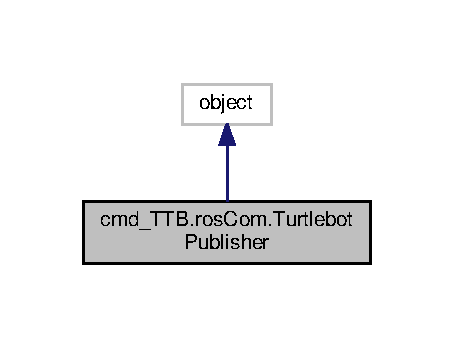
\includegraphics[width=218pt]{classcmd__TTB_1_1rosCom_1_1TurtlebotPublisher__inherit__graph}
\end{center}
\end{figure}


Collaboration diagram for cmd\+\_\+\+T\+T\+B.\+ros\+Com.\+Turtlebot\+Publisher\+:\nopagebreak
\begin{figure}[H]
\begin{center}
\leavevmode
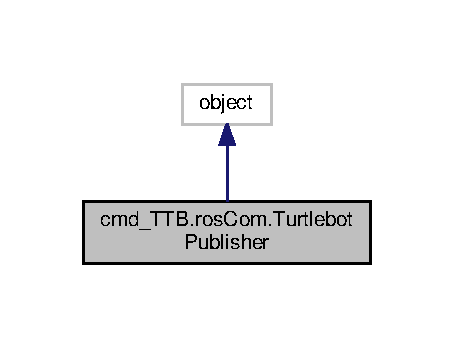
\includegraphics[width=218pt]{classcmd__TTB_1_1rosCom_1_1TurtlebotPublisher__coll__graph}
\end{center}
\end{figure}
\subsection*{Public Member Functions}
\begin{DoxyCompactItemize}
\item 
def \hyperlink{classcmd__TTB_1_1rosCom_1_1TurtlebotPublisher_a42833ada210e246fab7386110a43a934}{\+\_\+\+\_\+init\+\_\+\+\_\+} (self, F\+R\+E\+Q\+U\+E\+N\+CE=10)
\item 
def \hyperlink{classcmd__TTB_1_1rosCom_1_1TurtlebotPublisher_a157683d1e9db137dc27823546d901246}{send\+Command} (self, v, w)
\begin{DoxyCompactList}\small\item\em Send the desired velocities u and w to the robot as Twist. \end{DoxyCompactList}\item 
def \hyperlink{classcmd__TTB_1_1rosCom_1_1TurtlebotPublisher_aaabea5c15e3daa024cce879db332d0b1}{stop\+Smoothly} (self)
\item 
def \hyperlink{classcmd__TTB_1_1rosCom_1_1TurtlebotPublisher_a25af8f04357707576fa57d524860535b}{kill} (self)
\end{DoxyCompactItemize}
\subsection*{Public Attributes}
\begin{DoxyCompactItemize}
\item 
\hyperlink{classcmd__TTB_1_1rosCom_1_1TurtlebotPublisher_a14ff1a896341077ba1a89e7411078e0f}{publisher}
\item 
\hyperlink{classcmd__TTB_1_1rosCom_1_1TurtlebotPublisher_a98cdf1c16a60872288eb9acc94be2873}{rate}
\end{DoxyCompactItemize}


\subsection{Constructor \& Destructor Documentation}
\index{cmd\+\_\+\+T\+T\+B\+::ros\+Com\+::\+Turtlebot\+Publisher@{cmd\+\_\+\+T\+T\+B\+::ros\+Com\+::\+Turtlebot\+Publisher}!\+\_\+\+\_\+init\+\_\+\+\_\+@{\+\_\+\+\_\+init\+\_\+\+\_\+}}
\index{\+\_\+\+\_\+init\+\_\+\+\_\+@{\+\_\+\+\_\+init\+\_\+\+\_\+}!cmd\+\_\+\+T\+T\+B\+::ros\+Com\+::\+Turtlebot\+Publisher@{cmd\+\_\+\+T\+T\+B\+::ros\+Com\+::\+Turtlebot\+Publisher}}
\subsubsection[{\texorpdfstring{\+\_\+\+\_\+init\+\_\+\+\_\+(self, F\+R\+E\+Q\+U\+E\+N\+C\+E=10)}{__init__(self, FREQUENCE=10)}}]{\setlength{\rightskip}{0pt plus 5cm}def cmd\+\_\+\+T\+T\+B.\+ros\+Com.\+Turtlebot\+Publisher.\+\_\+\+\_\+init\+\_\+\+\_\+ (
\begin{DoxyParamCaption}
\item[{}]{self, }
\item[{}]{F\+R\+E\+Q\+U\+E\+N\+CE = {\ttfamily 10}}
\end{DoxyParamCaption}
)}\hypertarget{classcmd__TTB_1_1rosCom_1_1TurtlebotPublisher_a42833ada210e246fab7386110a43a934}{}\label{classcmd__TTB_1_1rosCom_1_1TurtlebotPublisher_a42833ada210e246fab7386110a43a934}


\subsection{Member Function Documentation}
\index{cmd\+\_\+\+T\+T\+B\+::ros\+Com\+::\+Turtlebot\+Publisher@{cmd\+\_\+\+T\+T\+B\+::ros\+Com\+::\+Turtlebot\+Publisher}!kill@{kill}}
\index{kill@{kill}!cmd\+\_\+\+T\+T\+B\+::ros\+Com\+::\+Turtlebot\+Publisher@{cmd\+\_\+\+T\+T\+B\+::ros\+Com\+::\+Turtlebot\+Publisher}}
\subsubsection[{\texorpdfstring{kill(self)}{kill(self)}}]{\setlength{\rightskip}{0pt plus 5cm}def cmd\+\_\+\+T\+T\+B.\+ros\+Com.\+Turtlebot\+Publisher.\+kill (
\begin{DoxyParamCaption}
\item[{}]{self}
\end{DoxyParamCaption}
)}\hypertarget{classcmd__TTB_1_1rosCom_1_1TurtlebotPublisher_a25af8f04357707576fa57d524860535b}{}\label{classcmd__TTB_1_1rosCom_1_1TurtlebotPublisher_a25af8f04357707576fa57d524860535b}
\begin{DoxyVerb}Doit etre appelée en fin de script si un publisher a ete cree\end{DoxyVerb}
 \index{cmd\+\_\+\+T\+T\+B\+::ros\+Com\+::\+Turtlebot\+Publisher@{cmd\+\_\+\+T\+T\+B\+::ros\+Com\+::\+Turtlebot\+Publisher}!send\+Command@{send\+Command}}
\index{send\+Command@{send\+Command}!cmd\+\_\+\+T\+T\+B\+::ros\+Com\+::\+Turtlebot\+Publisher@{cmd\+\_\+\+T\+T\+B\+::ros\+Com\+::\+Turtlebot\+Publisher}}
\subsubsection[{\texorpdfstring{send\+Command(self, v, w)}{sendCommand(self, v, w)}}]{\setlength{\rightskip}{0pt plus 5cm}def cmd\+\_\+\+T\+T\+B.\+ros\+Com.\+Turtlebot\+Publisher.\+send\+Command (
\begin{DoxyParamCaption}
\item[{}]{self, }
\item[{}]{v, }
\item[{}]{w}
\end{DoxyParamCaption}
)}\hypertarget{classcmd__TTB_1_1rosCom_1_1TurtlebotPublisher_a157683d1e9db137dc27823546d901246}{}\label{classcmd__TTB_1_1rosCom_1_1TurtlebotPublisher_a157683d1e9db137dc27823546d901246}


Send the desired velocities u and w to the robot as Twist. 

\index{cmd\+\_\+\+T\+T\+B\+::ros\+Com\+::\+Turtlebot\+Publisher@{cmd\+\_\+\+T\+T\+B\+::ros\+Com\+::\+Turtlebot\+Publisher}!stop\+Smoothly@{stop\+Smoothly}}
\index{stop\+Smoothly@{stop\+Smoothly}!cmd\+\_\+\+T\+T\+B\+::ros\+Com\+::\+Turtlebot\+Publisher@{cmd\+\_\+\+T\+T\+B\+::ros\+Com\+::\+Turtlebot\+Publisher}}
\subsubsection[{\texorpdfstring{stop\+Smoothly(self)}{stopSmoothly(self)}}]{\setlength{\rightskip}{0pt plus 5cm}def cmd\+\_\+\+T\+T\+B.\+ros\+Com.\+Turtlebot\+Publisher.\+stop\+Smoothly (
\begin{DoxyParamCaption}
\item[{}]{self}
\end{DoxyParamCaption}
)}\hypertarget{classcmd__TTB_1_1rosCom_1_1TurtlebotPublisher_aaabea5c15e3daa024cce879db332d0b1}{}\label{classcmd__TTB_1_1rosCom_1_1TurtlebotPublisher_aaabea5c15e3daa024cce879db332d0b1}
\begin{DoxyVerb}initialement prevue pour arreter delicatement le robot\end{DoxyVerb}
 

\subsection{Member Data Documentation}
\index{cmd\+\_\+\+T\+T\+B\+::ros\+Com\+::\+Turtlebot\+Publisher@{cmd\+\_\+\+T\+T\+B\+::ros\+Com\+::\+Turtlebot\+Publisher}!publisher@{publisher}}
\index{publisher@{publisher}!cmd\+\_\+\+T\+T\+B\+::ros\+Com\+::\+Turtlebot\+Publisher@{cmd\+\_\+\+T\+T\+B\+::ros\+Com\+::\+Turtlebot\+Publisher}}
\subsubsection[{\texorpdfstring{publisher}{publisher}}]{\setlength{\rightskip}{0pt plus 5cm}cmd\+\_\+\+T\+T\+B.\+ros\+Com.\+Turtlebot\+Publisher.\+publisher}\hypertarget{classcmd__TTB_1_1rosCom_1_1TurtlebotPublisher_a14ff1a896341077ba1a89e7411078e0f}{}\label{classcmd__TTB_1_1rosCom_1_1TurtlebotPublisher_a14ff1a896341077ba1a89e7411078e0f}
\index{cmd\+\_\+\+T\+T\+B\+::ros\+Com\+::\+Turtlebot\+Publisher@{cmd\+\_\+\+T\+T\+B\+::ros\+Com\+::\+Turtlebot\+Publisher}!rate@{rate}}
\index{rate@{rate}!cmd\+\_\+\+T\+T\+B\+::ros\+Com\+::\+Turtlebot\+Publisher@{cmd\+\_\+\+T\+T\+B\+::ros\+Com\+::\+Turtlebot\+Publisher}}
\subsubsection[{\texorpdfstring{rate}{rate}}]{\setlength{\rightskip}{0pt plus 5cm}cmd\+\_\+\+T\+T\+B.\+ros\+Com.\+Turtlebot\+Publisher.\+rate}\hypertarget{classcmd__TTB_1_1rosCom_1_1TurtlebotPublisher_a98cdf1c16a60872288eb9acc94be2873}{}\label{classcmd__TTB_1_1rosCom_1_1TurtlebotPublisher_a98cdf1c16a60872288eb9acc94be2873}


The documentation for this class was generated from the following file\+:\begin{DoxyCompactItemize}
\item 
\hyperlink{rosCom_8py}{ros\+Com.\+py}\end{DoxyCompactItemize}

\hypertarget{classTurtlebotPublisher}{}\section{Turtlebot\+Publisher Class Reference}
\label{classTurtlebotPublisher}\index{Turtlebot\+Publisher@{Turtlebot\+Publisher}}


R\+OS publisher in order to send the desired speeds (linear {\itshape u} and angular {\itshape w}) of the robot.  




\subsection{Detailed Description}
R\+OS publisher in order to send the desired speeds (linear {\itshape u} and angular {\itshape w}) of the robot. 


\begin{DoxyParams}{Parameters}
{\em F\+R\+E\+Q\+U\+E\+N\+CE} & Double Frequence of the control law \\
\hline
\end{DoxyParams}


The documentation for this class was generated from the following file\+:\begin{DoxyCompactItemize}
\item 
\hyperlink{rosCom_8py}{ros\+Com.\+py}\end{DoxyCompactItemize}

\chapter{File Documentation}
\hypertarget{____init_____8py}{}\section{\+\_\+\+\_\+init\+\_\+\+\_\+.\+py File Reference}
\label{____init_____8py}\index{\+\_\+\+\_\+init\+\_\+\+\_\+.\+py@{\+\_\+\+\_\+init\+\_\+\+\_\+.\+py}}
\subsection*{Namespaces}
\begin{DoxyCompactItemize}
\item 
 \hyperlink{namespacecmd__TTB}{cmd\+\_\+\+T\+TB}
\end{DoxyCompactItemize}

\hypertarget{butterworth_8py}{}\section{butterworth.\+py File Reference}
\label{butterworth_8py}\index{butterworth.\+py@{butterworth.\+py}}
\subsection*{Classes}
\begin{DoxyCompactItemize}
\item 
class \hyperlink{classcmd__TTB_1_1butterworth_1_1ButterworthFilter}{cmd\+\_\+\+T\+T\+B.\+butterworth.\+Butterworth\+Filter}
\end{DoxyCompactItemize}
\subsection*{Namespaces}
\begin{DoxyCompactItemize}
\item 
 \hyperlink{namespacecmd__TTB_1_1butterworth}{cmd\+\_\+\+T\+T\+B.\+butterworth}
\end{DoxyCompactItemize}

\hypertarget{cmd__ouverture_8py}{}\section{cmd\+\_\+ouverture.\+py File Reference}
\label{cmd__ouverture_8py}\index{cmd\+\_\+ouverture.\+py@{cmd\+\_\+ouverture.\+py}}


This script creates the necessary R\+OS services and actionlib in order to navigate the robot. It is the main file of the navigation.  


\subsection*{Namespaces}
\begin{DoxyCompactItemize}
\item 
 \hyperlink{namespacecmd__TTB_1_1cmd__ouverture}{cmd\+\_\+\+T\+T\+B.\+cmd\+\_\+ouverture}
\end{DoxyCompactItemize}
\subsection*{Functions}
\begin{DoxyCompactItemize}
\item 
def \hyperlink{namespacecmd__TTB_1_1cmd__ouverture_a69046dc4c4b699caef9e459f6620a389}{cmd\+\_\+\+T\+T\+B.\+cmd\+\_\+ouverture.\+handle\+Navigation} (req)
\begin{DoxyCompactList}\small\item\em Main function of the navigation, it computes the trajectory using \hyperlink{classPointCreator}{Point\+Creator} and \hyperlink{classTrajFactory}{Traj\+Factory}, then launches \hyperlink{namespacecmd__TTB_1_1cmd__ouverture_a265af166b80f6b0fd2414926197bd440}{follow\+Trajectory} that control the robot to follow it. \end{DoxyCompactList}\item 
def \hyperlink{namespacecmd__TTB_1_1cmd__ouverture_a265af166b80f6b0fd2414926197bd440}{cmd\+\_\+\+T\+T\+B.\+cmd\+\_\+ouverture.\+follow\+Trajectory} (trajectoire\+\_\+dans\+\_\+\+Rr, req, c\+Door, ttb\+Pose, initiale\+Rotation)
\begin{DoxyCompactList}\small\item\em Computes the controllers and launch the control law to follow the desired trajectory. \end{DoxyCompactList}\end{DoxyCompactItemize}
\subsection*{Variables}
\begin{DoxyCompactItemize}
\item 
\hyperlink{namespacecmd__TTB_1_1cmd__ouverture_a77e047b8c9fe806c29d099b045513d1e}{cmd\+\_\+\+T\+T\+B.\+cmd\+\_\+ouverture.\+anonymous}
\item 
int \hyperlink{namespacecmd__TTB_1_1cmd__ouverture_acccb0c5132d862843c65fc361ebbc8f4}{cmd\+\_\+\+T\+T\+B.\+cmd\+\_\+ouverture.\+F\+R\+E\+Q\+U\+E\+N\+CE} = 10
\begin{DoxyCompactList}\small\item\em Sample frequence of the robot. \end{DoxyCompactList}\item 
list \hyperlink{namespacecmd__TTB_1_1cmd__ouverture_af294464cb92aea691b05f1097a4ea28d}{cmd\+\_\+\+T\+T\+B.\+cmd\+\_\+ouverture.\+vel\+Max} = \mbox{[}0.\+25,0.\+2\mbox{]}
\begin{DoxyCompactList}\small\item\em Maximum velocities of the robot (linear in \mbox{[}m\mbox{]} then angular \mbox{[}rad\mbox{]}) \+: mbase values are \mbox{[}0.\+25 m/s, 0.\+1 rad/s\mbox{]}. \end{DoxyCompactList}\item 
\hyperlink{namespacecmd__TTB_1_1cmd__ouverture_a24119bb105d758e611e887c6d4c2a2b1}{cmd\+\_\+\+T\+T\+B.\+cmd\+\_\+ouverture.\+listener} = ros\+Com.\+Turtlebot\+Listener(\char`\"{}/odom\char`\"{},F\+R\+E\+Q\+U\+E\+N\+CE)
\begin{DoxyCompactList}\small\item\em Listener node from \hyperlink{namespacecmd__TTB_1_1rosCom}{ros\+Com}. \end{DoxyCompactList}\item 
\hyperlink{namespacecmd__TTB_1_1cmd__ouverture_a453ff2743ee8d9e0d8a9827f06ad3a4a}{cmd\+\_\+\+T\+T\+B.\+cmd\+\_\+ouverture.\+publisher} = ros\+Com.\+Turtlebot\+Publisher(F\+R\+E\+Q\+U\+E\+N\+CE)
\begin{DoxyCompactList}\small\item\em Publisher node from \hyperlink{namespacecmd__TTB_1_1rosCom}{ros\+Com}. \end{DoxyCompactList}\item 
\hyperlink{namespacecmd__TTB_1_1cmd__ouverture_ae3d69e9c63df8aea84f2ae92f853d24f}{cmd\+\_\+\+T\+T\+B.\+cmd\+\_\+ouverture.\+service} = rospy.\+Service(\textquotesingle{}navigation\+T\+TB\textquotesingle{}, navigation\+T\+TB, handle\+Navigation)
\end{DoxyCompactItemize}


\subsection{Detailed Description}
This script creates the necessary R\+OS services and actionlib in order to navigate the robot. It is the main file of the navigation. 

\begin{DoxyVersion}{Version}
1.\+3
\end{DoxyVersion}
Creates a listener node to get the datas from the robot and a publisher to send the control velocities. The navigation is handled by a R\+OS service (should be depreciated for an action\+Lib in 0.\+2) associated with the main function handle\+Navigation. This function receives the current steps and stages of the door opening from Goa\textquotesingle{}Uld, as well as the information on the door. From those informations, this function computes the desired trajectory and control the robot in order to follow it. 
\hypertarget{control_8py}{}\section{control.\+py File Reference}
\label{control_8py}\index{control.\+py@{control.\+py}}


Simplified version of Marc\textquotesingle{}s simulation\+\_\+functions.\+py.  


\subsection*{Namespaces}
\begin{DoxyCompactItemize}
\item 
 \hyperlink{namespacecmd__TTB_1_1control}{cmd\+\_\+\+T\+T\+B.\+control}
\end{DoxyCompactItemize}
\subsection*{Functions}
\begin{DoxyCompactItemize}
\item 
def \hyperlink{namespacecmd__TTB_1_1control_af6d33a997ba2c559550a999784957817}{cmd\+\_\+\+T\+T\+B.\+control.\+make\+References} (trajectory, ttb\+Pose, rotation\+Angle, F\+R\+EQ, vel\+Max)
\begin{DoxyCompactList}\small\item\em From the desired trajectory, computes the desired speeds and orientation of the robot. \end{DoxyCompactList}\item 
def \hyperlink{namespacecmd__TTB_1_1control_a3e268ec97147559f27deea1afe830d82}{cmd\+\_\+\+T\+T\+B.\+control.\+command\+Robot} (traj\+Size, turtlebot, C1, C2v, C2w, listener, publisher, traj\+Step)
\begin{DoxyCompactList}\small\item\em Control law of the robot. \end{DoxyCompactList}\end{DoxyCompactItemize}


\subsection{Detailed Description}
Simplified version of Marc\textquotesingle{}s simulation\+\_\+functions.\+py. 

\begin{DoxyVersion}{Version}
1.\+3 
\end{DoxyVersion}

\hypertarget{controllers_8py}{}\section{controllers.\+py File Reference}
\label{controllers_8py}\index{controllers.\+py@{controllers.\+py}}
\subsection*{Classes}
\begin{DoxyCompactItemize}
\item 
class \hyperlink{classcmd__TTB_1_1controllers_1_1TrajectoryStabilisator}{cmd\+\_\+\+T\+T\+B.\+controllers.\+Trajectory\+Stabilisator}
\item 
class \hyperlink{classcmd__TTB_1_1controllers_1_1turtlebotPID}{cmd\+\_\+\+T\+T\+B.\+controllers.\+turtlebot\+P\+ID}
\end{DoxyCompactItemize}
\subsection*{Namespaces}
\begin{DoxyCompactItemize}
\item 
 \hyperlink{namespacecmd__TTB_1_1controllers}{cmd\+\_\+\+T\+T\+B.\+controllers}
\end{DoxyCompactItemize}

\hypertarget{dataGatherer_8py}{}\section{data\+Gatherer.\+py File Reference}
\label{dataGatherer_8py}\index{data\+Gatherer.\+py@{data\+Gatherer.\+py}}
\subsection*{Classes}
\begin{DoxyCompactItemize}
\item 
class \hyperlink{classcmd__TTB_1_1dataGatherer_1_1DataGatherer}{cmd\+\_\+\+T\+T\+B.\+data\+Gatherer.\+Data\+Gatherer}
\end{DoxyCompactItemize}
\subsection*{Namespaces}
\begin{DoxyCompactItemize}
\item 
 \hyperlink{namespacecmd__TTB_1_1dataGatherer}{cmd\+\_\+\+T\+T\+B.\+data\+Gatherer}
\end{DoxyCompactItemize}

\hypertarget{door_8py}{}\section{door.\+py File Reference}
\label{door_8py}\index{door.\+py@{door.\+py}}
\subsection*{Classes}
\begin{DoxyCompactItemize}
\item 
class \hyperlink{classcmd__TTB_1_1door_1_1Door}{cmd\+\_\+\+T\+T\+B.\+door.\+Door}
\end{DoxyCompactItemize}
\subsection*{Namespaces}
\begin{DoxyCompactItemize}
\item 
 \hyperlink{namespacecmd__TTB_1_1door}{cmd\+\_\+\+T\+T\+B.\+door}
\end{DoxyCompactItemize}
\subsection*{Variables}
\begin{DoxyCompactItemize}
\item 
float \hyperlink{namespacecmd__TTB_1_1door_a464d4de3d59f16b66c790504e49d1fcc}{cmd\+\_\+\+T\+T\+B.\+door.\+l} = 0.\+60
\item 
float \hyperlink{namespacecmd__TTB_1_1door_a0de75fefbc56fabb9f68e23314b2451e}{cmd\+\_\+\+T\+T\+B.\+door.\+lp} = 0.\+13
\item 
float \hyperlink{namespacecmd__TTB_1_1door_abd3e267603515a4d02dd3b8e210ac96b}{cmd\+\_\+\+T\+T\+B.\+door.\+dis} = 0.\+05
\item 
float \hyperlink{namespacecmd__TTB_1_1door_ae04125c3c6ba7fdf00ead2a98493d716}{cmd\+\_\+\+T\+T\+B.\+door.\+e} = 0.\+04
\item 
float \hyperlink{namespacecmd__TTB_1_1door_a94ef176d5627a629b784bb8a6fda59df}{cmd\+\_\+\+T\+T\+B.\+door.\+r\+T\+TB} = 0.\+18
\end{DoxyCompactItemize}

\hypertarget{mainpage_8dox}{}\section{mainpage.\+dox File Reference}
\label{mainpage_8dox}\index{mainpage.\+dox@{mainpage.\+dox}}

\hypertarget{pointCreator_8py}{}\section{point\+Creator.\+py File Reference}
\label{pointCreator_8py}\index{point\+Creator.\+py@{point\+Creator.\+py}}
\subsection*{Classes}
\begin{DoxyCompactItemize}
\item 
class \hyperlink{classcmd__TTB_1_1pointCreator_1_1PointCreator}{cmd\+\_\+\+T\+T\+B.\+point\+Creator.\+Point\+Creator}
\end{DoxyCompactItemize}
\subsection*{Namespaces}
\begin{DoxyCompactItemize}
\item 
 \hyperlink{namespacecmd__TTB_1_1pointCreator}{cmd\+\_\+\+T\+T\+B.\+point\+Creator}
\end{DoxyCompactItemize}
\subsection*{Variables}
\begin{DoxyCompactItemize}
\item 
float \hyperlink{namespacecmd__TTB_1_1pointCreator_ac5dba97d9771fcc542d662e2c6304115}{cmd\+\_\+\+T\+T\+B.\+point\+Creator.\+D\+I\+S\+T2\+H\+A\+N\+D\+LE} = 0.\+1
\item 
int \hyperlink{namespacecmd__TTB_1_1pointCreator_a9cdfd77249436867b4079bfdb3df6682}{cmd\+\_\+\+T\+T\+B.\+point\+Creator.\+A\+L\+P\+H\+A\+\_\+\+O\+P\+EN} = np.\+pi/2
\end{DoxyCompactItemize}

\hypertarget{rosCom_8py}{}\section{ros\+Com.\+py File Reference}
\label{rosCom_8py}\index{ros\+Com.\+py@{ros\+Com.\+py}}
\subsection*{Classes}
\begin{DoxyCompactItemize}
\item 
class \hyperlink{classcmd__TTB_1_1rosCom_1_1TurtlebotListener}{cmd\+\_\+\+T\+T\+B.\+ros\+Com.\+Turtlebot\+Listener}
\item 
class \hyperlink{classcmd__TTB_1_1rosCom_1_1TurtlebotPublisher}{cmd\+\_\+\+T\+T\+B.\+ros\+Com.\+Turtlebot\+Publisher}
\end{DoxyCompactItemize}
\subsection*{Namespaces}
\begin{DoxyCompactItemize}
\item 
 \hyperlink{namespacecmd__TTB_1_1rosCom}{cmd\+\_\+\+T\+T\+B.\+ros\+Com}
\end{DoxyCompactItemize}

\hypertarget{trajFactory_8py}{}\section{traj\+Factory.\+py File Reference}
\label{trajFactory_8py}\index{traj\+Factory.\+py@{traj\+Factory.\+py}}
\subsection*{Classes}
\begin{DoxyCompactItemize}
\item 
class \hyperlink{classcmd__TTB_1_1trajFactory_1_1TrajFactory}{cmd\+\_\+\+T\+T\+B.\+traj\+Factory.\+Traj\+Factory}
\end{DoxyCompactItemize}
\subsection*{Namespaces}
\begin{DoxyCompactItemize}
\item 
 \hyperlink{namespacecmd__TTB_1_1trajFactory}{cmd\+\_\+\+T\+T\+B.\+traj\+Factory}
\end{DoxyCompactItemize}
\subsection*{Variables}
\begin{DoxyCompactItemize}
\item 
\hyperlink{namespacecmd__TTB_1_1trajFactory_a155b2c6da96a917f0ac2ad1b45e68f65}{cmd\+\_\+\+T\+T\+B.\+traj\+Factory.\+points} = random\+Points\+Creator(4)
\item 
int \hyperlink{namespacecmd__TTB_1_1trajFactory_abb2e2587a58c4fc35dd18e79526c3a67}{cmd\+\_\+\+T\+T\+B.\+traj\+Factory.\+freq} = 10
\item 
float \hyperlink{namespacecmd__TTB_1_1trajFactory_a31f0c63eecd9cb034f7db3c30fc94a1b}{cmd\+\_\+\+T\+T\+B.\+traj\+Factory.\+coef\+Tan} = 1.\+5
\item 
int \hyperlink{namespacecmd__TTB_1_1trajFactory_ac0c9d7799ff61a3cfe3128872918c3d2}{cmd\+\_\+\+T\+T\+B.\+traj\+Factory.\+thetaF} = 0
\item 
list \hyperlink{namespacecmd__TTB_1_1trajFactory_aa5408e0df737a89e02b70bae38dabdf5}{cmd\+\_\+\+T\+T\+B.\+traj\+Factory.\+Pf} = \mbox{[}1.\+4,0.\+4\mbox{]}
\item 
list \hyperlink{namespacecmd__TTB_1_1trajFactory_a99ccef9f51bec12c2c7ed06cb5dd9d3a}{cmd\+\_\+\+T\+T\+B.\+traj\+Factory.\+Pf1} = \mbox{[}Pf\mbox{[}0\mbox{]}-\/coef\+Tan$\ast$math.\+cos(thetaF), Pf\mbox{[}1\mbox{]}-\/coef\+Tan$\ast$math.\+sin(thetaF)\mbox{]}
\item 
float \hyperlink{namespacecmd__TTB_1_1trajFactory_a40f972381ea23fa3614767994e20909e}{cmd\+\_\+\+T\+T\+B.\+traj\+Factory.\+dt} = 0.\+1
\item 
float \hyperlink{namespacecmd__TTB_1_1trajFactory_a25697213c9c1b12b56e1d9cb2b488f6d}{cmd\+\_\+\+T\+T\+B.\+traj\+Factory.\+vitesse\+Max} = 0.\+1
\item 
\hyperlink{namespacecmd__TTB_1_1trajFactory_a377dd717e6d99f94f3bd8359315ce8f2}{cmd\+\_\+\+T\+T\+B.\+traj\+Factory.\+path} = \hyperlink{classTrajFactory}{Traj\+Factory}(points,freq,100)
\item 
\hyperlink{namespacecmd__TTB_1_1trajFactory_ac955d640aed48051089654bf294a2001}{cmd\+\_\+\+T\+T\+B.\+traj\+Factory.\+xvals}
\item 
\hyperlink{namespacecmd__TTB_1_1trajFactory_a7a877f7cdb271eb3276d034ab078d600}{cmd\+\_\+\+T\+T\+B.\+traj\+Factory.\+yvals}
\item 
\hyperlink{namespacecmd__TTB_1_1trajFactory_a6c2b69f01c79170fee15a08f7d7be3c5}{cmd\+\_\+\+T\+T\+B.\+traj\+Factory.\+speeds}
\item 
\hyperlink{namespacecmd__TTB_1_1trajFactory_a3d3e3185576a4d8c1f41771d38dae565}{cmd\+\_\+\+T\+T\+B.\+traj\+Factory.\+wspeeds}
\item 
\hyperlink{namespacecmd__TTB_1_1trajFactory_a9d34c2505734ce41d485698c66d3af36}{cmd\+\_\+\+T\+T\+B.\+traj\+Factory.\+xvalsB}
\item 
\hyperlink{namespacecmd__TTB_1_1trajFactory_a445a9f003e3be237b7176463d2ae0ca8}{cmd\+\_\+\+T\+T\+B.\+traj\+Factory.\+yvalsB}
\item 
\hyperlink{namespacecmd__TTB_1_1trajFactory_a4eb9c241c592b3fbf3c824c82e0397d4}{cmd\+\_\+\+T\+T\+B.\+traj\+Factory.\+f}
\item 
\hyperlink{namespacecmd__TTB_1_1trajFactory_aa4dac444c1fe3126aca359b6d54026dc}{cmd\+\_\+\+T\+T\+B.\+traj\+Factory.\+axarr}
\item 
\hyperlink{namespacecmd__TTB_1_1trajFactory_a9b3b7658cef42597751a680874ba240a}{cmd\+\_\+\+T\+T\+B.\+traj\+Factory.\+ax} = plt.\+gca()
\end{DoxyCompactItemize}

\hypertarget{utils_8py}{}\section{utils.\+py File Reference}
\label{utils_8py}\index{utils.\+py@{utils.\+py}}


All functions that might be used by any other functions for computing or mathematical purposes.  


\subsection*{Classes}
\begin{DoxyCompactItemize}
\item 
class \hyperlink{classcmd__TTB_1_1utils_1_1Smoother}{cmd\+\_\+\+T\+T\+B.\+utils.\+Smoother}
\end{DoxyCompactItemize}
\subsection*{Namespaces}
\begin{DoxyCompactItemize}
\item 
 \hyperlink{namespacecmd__TTB_1_1utils}{cmd\+\_\+\+T\+T\+B.\+utils}
\end{DoxyCompactItemize}
\subsection*{Functions}
\begin{DoxyCompactItemize}
\item 
def \hyperlink{namespacecmd__TTB_1_1utils_a59935c2b4ec8161367ca748f99c376cf}{cmd\+\_\+\+T\+T\+B.\+utils.\+lifted\+Atan2} (consigne\+\_\+vx, consigne\+\_\+vy)
\begin{DoxyCompactList}\small\item\em Computes the atan value of each elements of two arrays and lifts it. \end{DoxyCompactList}\end{DoxyCompactItemize}


\subsection{Detailed Description}
All functions that might be used by any other functions for computing or mathematical purposes. 

\begin{DoxyVersion}{Version}
1.\+3 
\end{DoxyVersion}

%--- End generated contents ---

% Index
\backmatter
\newpage
\phantomsection
\clearemptydoublepage
\addcontentsline{toc}{chapter}{Index}
\printindex

\end{document}
